\title{统计与概率（2016--2025 高考真题）}
\author{}
\date{}
\maketitle
\noindent 本专题共 167 道题，按年份排列。每题标注原卷与原题号。

\section*{2016 年}

\begin{question}[points=5]
\textbf{来源：}2016 年 全国III卷-理科，第 4 题\par
某旅游城市为向游客介绍本地的气温情况, 绘制了一年中各月平均最高气温和平均最低气温的雷达图, 图中 $A$ 点表示十月的平均最高气温约为 $15^\circ\mathrm{C}$, $B$ 点表示四月的平均最低气温约为 $5^\circ\mathrm{C}$, 下面叙述不正确的是

\begin{center}
  
\includegraphics[width=.42\linewidth]{assets/asset-001-01.jpg}
\end{center}
\begin{choices}
  \item 各月的平均最低气温都在 $0^\circ\mathrm{C}$ 以上
  \item 七月的平均温差比一月的平均温差大
  \item 三月和十一月的平均最高气温基本相同
  \item 平均最高气温高于 $20^\circ\mathrm{C}$ 的月份有 $5$ 个
\end{choices}
\begin{solution}
\textbf{答案：}平均最高气温高于 $20^\circ\mathrm{C}$ 的月份有 $5$ 个

\textbf{分析：}根据平均最高气温和平均最低气温的雷达图进行推理判断.

\textbf{详解：}A. 由雷达图知各月的平均最低气温都在 $0^\circ\mathrm{C}$ 以上, 正确. B. 七月的平均温差大约在 $10^\circ$ 左右, 一月的平均温差在 $5^\circ$ 左右, 故七月的平均温差比一月的平均温差大, 正确. C. 三月和十一月的平均最高气温基本相同, 都为 $10^\circ$, 正确. D. 平均最高气温高于 $20^\circ\mathrm{C}$ 的月份有 $7,8$ 两个月, 故 D 错误, 故选 D.
\end{solution}
\end{question}

\begin{question}[points=12]
\textbf{来源：}2016 年 全国III卷-理科，第 18 题\par
如图是我国2008年至2014年生活垃圾无害化处理量（单位：亿吨）的折线图.

注：年份代码 $1\!-\!7$ 分别对应年份2008～2014.

(Ⅰ) 由折线图看出, 可用线性回归模型拟合 $y$ 与 $t$ 的关系, 请用相关系数加以证明;

(Ⅱ) 建立 $y$ 关于 $t$ 的回归方程（系数精确到 $0.01$）, 预测2016年我国生活垃圾无害化处理量.

附注：参考数据 $\sum_{i=1}^{7}y_i=9.32$, $\sum_{i=1}^{7}t_iy_i=40.17$, $\sqrt{\sum_{i=1}^{7}(y_i-\bar{y})^2}=0.55$, $\sqrt{7}\approx2.646$.

参考公式：相关系数 $r=\frac{\sum_{i=1}^{n}(t_i-\bar{t})(y_i-\bar{y})}{\sqrt{\sum_{i=1}^{n}(t_i-\bar{t})^2\sum_{i=1}^{n}(y_i-\bar{y})^2}}$, 回归方程 $\hat{y}=\hat{b}t+\hat{a}$ 中斜率和截距的最小二乘估计公式分别为 $\hat{b}=\frac{\sum_{i=1}^{n}(t_i-\bar{t})(y_i-\bar{y})}{\sum_{i=1}^{n}(t_i-\bar{t})^2}$, $\hat{a}=\bar{y}-\hat{b}\bar{t}$.

\begin{center}
  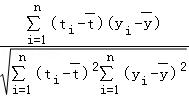
\includegraphics[width=.42\linewidth]{assets/asset-002-01.jpg}
\end{center}
\begin{solution}

\textbf{分析：}(1) 由折线图看出 $y$ 与 $t$ 之间存在较强的正相关关系, 将已知数据代入相关系数方程可得答案. (2) 根据已知数据求出回归系数, 可得回归方程, 2016年对应的 $t$ 值为 $9$, 代入可预测.

\textbf{详解：}(Ⅰ) 由折线图看出, $y$ 与 $t$ 之间存在较强的正相关关系, 理由如下: $\because r=\frac{\sum_{i=1}^{7}(t_i-\bar{t})(y_i-\bar{y})}{\sqrt{\sum_{i=1}^{7}(t_i-\bar{t})^2\sum_{i=1}^{7}(y_i-\bar{y})^2}}=\frac{\sum_{i=1}^{7}t_iy_i-7\bar{t}\bar{y}}{\sqrt{(\sum_{i=1}^{7}t_i^2-7\bar{t}^2)\sum_{i=1}^{7}(y_i-\bar{y})^2}}=\frac{40.17-7\times4\times\frac{9.32}{7}}{\sqrt{(28-7\times4^2)\times0.55^2}}=\frac{40.17-4\times9.32}{\sqrt{0\text{?}}}$? 注意: $\sum t_i=1+2+\cdots+7=28$, $\bar{t}=4$, $\bar{y}=9.32/7\approx1.331$. $\sum t_i^2=1^2+2^2+\cdots+7^2=140$. 实际计算: $r=\frac{40.17-7\times4\times1.331}{\sqrt{(140-7\times16)\times0.55^2}}=\frac{40.17-37.268}{\sqrt{(140-112)\times0.3025}}=\frac{2.902}{\sqrt{28\times0.3025}}=\frac{2.902}{\sqrt{8.47}}\approx\frac{2.902}{2.91}\approx0.997$? 原解析为 $\approx0.993$. 按原文: $\because r\approx0.993>0.75$, 故 $y$ 与 $t$ 之间存在较强的正相关关系.
(Ⅱ) $\hat{b}=\frac{\sum_{i=1}^{7}(t_i-\bar{t})(y_i-\bar{y})}{\sum_{i=1}^{7}(t_i-\bar{t})^2}=\frac{40.17-7\times4\times1.331}{28}\approx\frac{2.902}{28}\approx0.103$, $\hat{a}=\bar{y}-\hat{b}\bar{t}\approx1.331-0.103\times4\approx0.92$, $\therefore y$ 关于 $t$ 的回归方程为 $\hat{y}=0.10t+0.92$. 2016年对应的 $t$ 值为 $9$, 故 $\hat{y}=0.10\times9+0.92=1.82$, 预测2016年我国生活垃圾无害化处理量为 $1.82$ 亿吨.
\end{solution}
\end{question}

\begin{question}[points=5]
\textbf{来源：}2016 年 全国III卷-文科，第 4 题\par
某旅游城市为向游客介绍本地的气温情况, 绘制了一年中各月平均最高气温和平均最低气温的雷达图, 图中 $A$ 点表示十月的平均最高气温约为 $15^{\circ}C$, $B$ 点表示四月的平均最低气温约为 $5^{\circ}C$, 下面叙述不正确的是 ( )

\begin{center}
  
\includegraphics[width=.42\linewidth]{assets/asset-003-01.jpg}
\end{center}
\begin{choices}
  \item 各月的平均最低气温都在 $0^{\circ}C$ 以上
  \item 七月的平均温差比一月的平均温差大
  \item 三月和十一月的平均最高气温基本相同
  \item 平均最高气温高于 $20^{\circ}C$ 的月份有 $5$ 个
\end{choices}
\begin{solution}
\textbf{答案：}平均最高气温高于 $20^{\circ}C$ 的月份有 $5$ 个

\textbf{分析：}根据平均最高气温和平均最低气温的雷达图进行推理判断即可.

\textbf{详解：}A. 由雷达图知各月的平均最低气温都在 $0^{\circ}C$ 以上, 正确. B. 七月的平均温差大约在 $10^{\circ}$ 左右, 一月的平均温差在 $5^{\circ}$ 左右, 故七月的平均温差比一月的平均温差大, 正确. C. 三月和十一月的平均最高气温基本相同, 都为 $10^{\circ}$, 正确. D. 平均最高气温高于 $20^{\circ}C$ 的月份有 $7,8$ 两个月, 故 D 错误. 故选 D.
\end{solution}
\end{question}

\begin{question}[points=5]
\textbf{来源：}2016 年 全国III卷-文科，第 5 题\par
小敏打开计算机时, 忘记了开机密码的前两位, 只记得第一位是 $M$, $I$, $N$ 中的一个字母, 第二位是 $1$, $2$, $3$, $4$, $5$ 中的一个数字, 则小敏输入一次密码能够成功开机的概率是 ( )
\begin{choices}
  \item $\dfrac{1}{15}$
  \item $\dfrac{1}{8}$
  \item $\dfrac{1}{15}$
  \item $\dfrac{1}{30}$
\end{choices}
\begin{solution}
\textbf{答案：}$\dfrac{1}{15}$

\textbf{分析：}列举出从 $M$, $I$, $N$ 中任取一个字母, 再从 $1$, $2$, $3$, $4$, $5$ 中任取一个数字的基本事件数, 然后由随机事件发生的概率得答案.

\textbf{详解：}从 $M$, $I$, $N$ 中任取一个字母, 再从 $1$, $2$, $3$, $4$, $5$ 中任取一个数字, 取法总数为 $(M,1),(M,2),(M,3),(M,4),(M,5),(I,1),(I,2),(I,3),(I,4),(I,5),(N,1),(N,2),(N,3),(N,4),(N,5)$ 共 $15$ 种. 其中只有一个是小敏的密码前两位. 由随机事件发生的概率可得, 小敏输入一次密码能够成功开机的概率是 $\dfrac{1}{15}$. 故选 C.
\end{solution}
\end{question}

\begin{question}[points=12]
\textbf{来源：}2016 年 全国III卷-文科，第 18 题\par
如图是我国 2008 年至 2014 年生活垃圾无害化处理量 (单位: 亿吨) 的折线图. 注: 年份代码 $1-7$ 分别对应年份 $2008-2014$.

(Ⅰ) 由折线图看出, 可用线性回归模型拟合 $y$ 与 $t$ 的关系, 请用相关系数加以证明;

(Ⅱ) 建立 $y$ 关于 $t$ 的回归方程 (系数精确到 $0.01$), 预测 $2016$ 年我国生活垃圾无害化处理量.

附注:

参考数据: $\sum_{i=1}^{7}y_i=9.32$, $\sum_{i=1}^{7}t_iy_i=40.17$, $\sqrt{\sum_{i=1}^{7}(y_i-\bar{y})^2}=0.55$, $\sqrt{7}\approx2.646$.

参考公式: 相关系数 $r=\dfrac{\sum_{i=1}^{n}(t_i-\bar{t})(y_i-\bar{y})}{\sqrt{\sum_{i=1}^{n}(t_i-\bar{t})^2}\sqrt{\sum_{i=1}^{n}(y_i-\bar{y})^2}}$, 回归方程 $\hat{y}=\hat{b}+\hat{a}t$ 中斜率和截距的最小二乘估计公式分别为 $\hat{b}=\dfrac{\sum_{i=1}^{n}(t_i-\bar{t})(y_i-\bar{y})}{\sum_{i=1}^{n}(t_i-\bar{t})^2}$, $\hat{a}=\bar{y}-\hat{b}\bar{t}$.

\begin{center}
  
\includegraphics[width=.42\linewidth]{assets/asset-005-01.jpg}
\end{center}
\begin{solution}
\textbf{答案：}见解析

\textbf{分析：}(1) 由折线图看出, $y$ 与 $t$ 之间存在较强的正相关关系, 将已知数据代入相关系数方程, 可得答案; (2) 根据已知中的数据, 求出回归系数, 可得回归方程, $2016$ 年对应的 $t$ 值为 $9$, 代入可预测 $2016$ 年我国生活垃圾无害化处理量.

\textbf{详解：}(Ⅰ) 由折线图得 $\bar{t}=\frac{1+2+\cdots+7}{7}=4$, $\sum_{i=1}^{7}(t_i-\bar{t})^2=28$. $\sum_{i=1}^{7}(t_i-\bar{t})(y_i-\bar{y})=\sum_{i=1}^{7}t_iy_i-\bar{t}\sum_{i=1}^{7}y_i=40.17-4\times9.32=40.17-37.28=2.89$. $\sqrt{\sum_{i=1}^{7}(y_i-\bar{y})^2}=0.55$, $\sqrt{\sum_{i=1}^{7}(t_i-\bar{t})^2}=\sqrt{28}=2\sqrt{7}\approx2\times2.646=5.292$. 所以 $r=\dfrac{2.89}{5.292\times0.55}\approx\dfrac{2.89}{2.9106}\approx0.993$. 因为 $0.993>0.75$, 故 $y$ 与 $t$ 之间存在较强的正相关关系.
(Ⅱ) $\hat{b}=\dfrac{2.89}{28}\approx0.103$, $\bar{y}=\dfrac{9.32}{7}\approx1.331$, $\hat{a}=\bar{y}-\hat{b}\bar{t}\approx1.331-0.103\times4=0.92$. 所以 $y$ 关于 $t$ 的回归方程为 $\hat{y}=0.10t+0.92$. $2016$ 年对应的 $t=9$, 代入得 $\hat{y}=0.10\times9+0.92=1.82$. 所以预测 $2016$ 年我国生活垃圾无害化处理量为 $1.82$ 亿吨.
\end{solution}
\end{question}

\begin{question}[points=5]
\textbf{来源：}2016 年 全国II卷-理科，第 10 题\par
从区间$[0,1]$随机抽取$2n$个数$x_1,x_2,\ldots,x_n$，$y_1,y_2,\ldots,y_n$构成$n$个数对$(x_1,y_1)$，$(x_2,y_2)$，$\ldots$，$(x_n,y_n)$，其中两数的平方和小于$1$的数对共有$m$个，则用随机模拟的方法得到的圆周率$\pi$的近似值为（\quad）
\begin{choices}
  \item $\frac{4n}{m}$
  \item $\frac{2n}{m}$
  \item $\frac{4m}{n}$
  \item $\frac{2m}{n}$
\end{choices}
\begin{solution}
\textbf{答案：}$\frac{4m}{n}$

\textbf{分析：}以面积为测度，建立方程，即可求出圆周率$\pi$的近似值．

\textbf{详解：}由几何概型，$\frac{m}{n}=\frac{\frac{1}{4}\pi\times1^2}{1^2}$，解得$\pi=\frac{4m}{n}$．故选C．
\end{solution}
\end{question}

\begin{question}[points=12]
\textbf{来源：}2016 年 全国II卷-理科，第 18 题\par
某保险的基本保费为$a$（单位：元），继续购买该保险的投保人成为续保人，续保人本年度的保费与其上年度出险次数的关联如下：



| 上年度出险次数 | 0 | 1 | 2 | 3 | 4 | $\ge5$ |

|----------------|---|---|---|---|---|--------|

| 保费 | $0.85a$ | $a$ | $1.25a$ | $1.5a$ | $1.75a$ | $2a$ |



设该险种一续保人一年内出险次数与相应概率如下：



| 一年内出险次数 | 0 | 1 | 2 | 3 | 4 | $\ge5$ |

|----------------|---|---|---|---|---|--------|

| 概率 | $0.30$ | $0.15$ | $0.20$ | $0.20$ | $0.10$ | $0.05$ |



（Ⅰ）求一续保人本年度的保费高于基本保费的概率；

（Ⅱ）若一续保人本年度的保费高于基本保费，求其保费比基本保费高出$60\%$的概率；

（Ⅲ）求续保人本年度的平均保费与基本保费的比值．
\begin{solution}
\textbf{答案：}（Ⅰ）$0.55$；（Ⅱ）$\frac{3}{11}$；（Ⅲ）$1.23$

\textbf{分析：}（Ⅰ）上年度出险次数大于等于2时，续保人本年度的保费高于基本保费，由此利用该险种一续保人一年内出险次数与相应概率统计表根据对立事件概率计算公式能求出一续保人本年度的保费高于基本保费的概率．（Ⅱ）设事件A表示“一续保人本年度的保费高于基本保费”，事件B表示“一续保人本年度的保费比基本保费高出60%”，由题意求出$P(A)$，$P(AB)$，由此利用条件概率能求出若一续保人本年度的保费高于基本保费，则其保费比基本保费高出60%的概率．（Ⅲ）由题意，能求出续保人本年度的平均保费与基本保费的比值．

\textbf{详解：}（Ⅰ）$P=1-0.30-0.15=0.55$．
（Ⅱ）设事件A：保费高于基本保费，事件B：保费比基本保费高出60%，则$P(A)=0.55$，$P(AB)=0.10+0.05=0.15$，$P(B|A)=\frac{0.15}{0.55}=\frac{3}{11}$．
（Ⅲ）平均保费$E=0.85a\times0.30+a\times0.15+1.25a\times0.20+1.5a\times0.20+1.75a\times0.10+2a\times0.05=1.23a$，比值为$1.23$．
\end{solution}
\end{question}

\begin{question}[points=5]
\textbf{来源：}2016 年 全国II卷-文科，第 8 题\par
某路口人行横道的信号灯为红灯和绿灯交替出现，红灯持续时间为40秒。若一名行人来到该路口遇到红灯，则至少需要等待15秒才出现绿灯的概率为
\begin{choices}
  \item $\frac{1}{2}$
  \item $\frac{5}{8}$
  \item $\frac{3}{8}$
  \item $\frac{3}{10}$
\end{choices}
\begin{solution}
\textbf{答案：}$\frac{5}{8}$

\textbf{分析：}红灯持续40秒，至少等15秒，则需在前25秒内到达，概率$\frac{25}{40}=\frac{5}{8}$。
\end{solution}
\end{question}

\begin{question}[points=5]
\textbf{来源：}2016 年 全国II卷-文科，第 9 题\par
中国古代有计算多项式值的秦九韶算法，如图是实现该算法的程序框图。执行该程序框图，若输入的$x=2$，$n=2$，依次输入的$a$为2，2，5，则输出的$s=$

\begin{center}
  
\includegraphics[width=.42\linewidth]{assets/asset-009-01.jpg}
\end{center}
\begin{choices}
  \item $7$
  \item $12$
  \item $17$
  \item $34$
\end{choices}
\begin{solution}
\textbf{答案：}$17$

\textbf{分析：}模拟：$k=1$，$s=0\times2+2=2$；$k=2$，$s=2\times2+2=6$；$k=3$，$s=6\times2+5=17$，输出$s=17$。
\end{solution}
\end{question}

\begin{question}[points=5]
\textbf{来源：}2016 年 全国II卷-文科，第 16 题\par
有三张卡片，分别写有1和2，1和3，2和3。甲，乙，丙三人各取走一张卡片，甲看了乙的卡片后说：“我与乙的卡片上相同的数字不是2”，乙看了丙的卡片后说：“我与丙的卡片上相同的数字不是1”，丙说：“我的卡片上的数字之和不是5”，则甲的卡片上的数字是
\fillin[{$1$和$3$}]
\begin{solution}
\textbf{答案：}$1$和$3$

\textbf{分析：}推理得甲卡片上的数字是1和3。
\end{solution}
\end{question}

\begin{question}[points=12]
\textbf{来源：}2016 年 全国II卷-文科，第 18 题\par
某险种的基本保费为$a$（单位：元），继续购买该险种的投保人称为续保人，续保人本年度的保费与其上年度出险次数的关联如下：



上年度出险次数$\quad0\quad1\quad2\quad3\quad4\quad\ge5$

保费$\quad0.85a\quad a\quad1.25a\quad1.5a\quad1.75a\quad2a$



随机调查了该险种的200名续保人在一年内的出险情况，得到如下统计表：



出险次数$\quad0\quad1\quad2\quad3\quad4\quad\ge5$

频数$\quad60\quad50\quad30\quad30\quad20\quad10$



（Ⅰ）记$A$为事件：“一续保人本年度的保费不高于基本保费”。求$P(A)$的估计值；

（Ⅱ）记$B$为事件：“一续保人本年度的保费高于基本保费但不高于基本保费的160%”。求$P(B)$的估计值；

（Ⅲ）求续保人本年度的平均保费估计值。
\begin{solution}
\textbf{答案：}（Ⅰ）$\frac{11}{20}$；（Ⅱ）$\frac{3}{10}$；（Ⅲ）$1.1925a$

\textbf{分析：}（Ⅰ）保费不高于基本保费的人数$60+50=110$，$P(A)=\frac{110}{200}=\frac{11}{20}$。
（Ⅱ）保费高于基本保费但不高于$1.6a$的人数$30+30=60$，$P(B)=\frac{60}{200}=\frac{3}{10}$。
（Ⅲ）平均保费$=\frac{0.85a\times60+a\times50+1.25a\times30+1.5a\times30+1.75a\times20+2a\times10}{200}=1.1925a$。
\end{solution}
\end{question}

\begin{question}[points=5]
\textbf{来源：}2016 年 全国I卷-理科，第 4 题\par
某公司的班车在7:00，8:00，8:30发车，小明在7:50至8:30之间到达发车站乘坐班车，且到达发车站的时刻是随机的，则他等车时间不超过10分钟的概率是（ ）
\begin{choices}
  \item $\frac{1}{3}$
  \item $\frac{1}{2}$
  \item $\frac{2}{3}$
  \item $\frac{3}{4}$
\end{choices}
\begin{solution}
\textbf{答案：}B

\textbf{分析：}求出小明等车时间不超过10分钟的时间长度，代入几何概型概率计算公式，可得答案．

\textbf{详解：}解：设小明到达时间为$y$，当$y$在7:50至8:00，或8:20至8:30时，小明等车时间不超过10分钟，故$P=\frac{40}{40}=\frac{1}{2}$，故选：B．
\end{solution}
\end{question}

\begin{question}[points=5]
\textbf{来源：}2016 年 全国I卷-理科，第 9 题\par
执行下面的程序框图，如果输入的$x=0$，$y=1$，$n=1$，则输出$x$，$y$的值满足（ ）

\begin{center}
  
\includegraphics[width=.42\linewidth]{assets/asset-013-01.jpg}
\end{center}
\begin{choices}
  \item $y=2x$
  \item $y=3x$
  \item $y=4x$
  \item $y=5x$
\end{choices}
\begin{solution}
\textbf{答案：}C

\textbf{分析：}由已知中的程序框图可知：该程序的功能是利用循环结构计算并输出变量$x$，$y$的值，模拟程序的运行过程，分析循环中各变量值的变化情况，可得答案．

\textbf{详解：}解：输入$x=0$，$y=1$，$n=1$，则$x=0$，$y=1$，不满足$x^2+y^2\ge36$，故$n=2$，则$x=\frac{1}{2}$，$y=2$，不满足$x^2+y^2\ge36$，故$n=3$，则$x=\frac{3}{2}$，$y=6$，满足$x^2+y^2\ge36$，故$y=4x$，故选：$C$．
\end{solution}
\end{question}

\begin{question}[points=12]
\textbf{来源：}2016 年 全国I卷-理科，第 19 题\par
某公司计划购买$2$台机器，该种机器使用三年后即被淘汰．机器有一易损零件，在购进机器时，可以额外购买这种零件作为备件，每个$200$元．在机器使用期间，如果备件不足再购买，则每个$500$元．现需决策在购买机器时应同时购买几个易损零件，为此搜集并整理了$100$台这种机器在三年使用期内更换的易损零件数，得如图柱状图：以这$100$台机器更换的易损零件数的频率代替$1$台机器更换的易损零件数发生的概率，记$X$表示$2$台机器三年内共需更换的易损零件数，$n$表示购买$2$台机器的同时购买的易损零件数．

（Ⅰ）求$X$的分布列；

（Ⅱ）若要求$P(X\le n)\ge0.5$，确定$n$的最小值；

（Ⅲ）以购买易损零件所需费用的期望值为决策依据，在$n=19$与$n=20$之中选其一，应选用哪个？

\begin{center}
  
\includegraphics[width=.42\linewidth]{assets/asset-014-01.jpg}
\end{center}
\begin{solution}
\textbf{答案：}（Ⅰ）分布列见解析；（Ⅱ）$n$的最小值为$19$；（Ⅲ）应选$n=19$

\textbf{分析：}（Ⅰ）由已知得$X$的可能取值为$16$，$17$，$18$，$19$，$20$，$21$，$22$，分别求出相应的概率，由此能求出$X$的分布列．（Ⅱ）由$X$的分布列求出$P(X\le18)=\frac{3}{10}$，$P(X\le19)=\frac{7}{10}$．由此能确定满足$P(X\le n)\ge0.5$中$n$的最小值．（Ⅲ）法一：由$X$的分布列得$P(X\le19)=\frac{7}{10}$．求出买$19$个所需费用期望$EX_1$和买$20$个所需费用期望$EX_2$，由此能求出买$19$个更合适．法二：购买零件所用费用含两部分，一部分为购买零件的费用，另一部分为备件不足时额外购买的费用，分别求出$n=19$时，费用的期望和当$n=20$时，费用的期望，从而得到买$19$个更合适．

\textbf{详解：}解：（Ⅰ）由已知得$X$的可能取值为$16$，$17$，$18$，$19$，$20$，$21$，$22$，$P(X=16)=(\frac{20}{100})^2=\frac{1}{25}$，$P(X=17)=2\times\frac{20}{100}\times\frac{20}{100}=\frac{2}{25}$，$P(X=18)=(\frac{20}{100})^2+2\times(\frac{20}{100})^2=\frac{3}{25}$，$P(X=19)=2\times\frac{20}{100}\times\frac{40}{100}+2\times\frac{20}{100}\times\frac{20}{100}=\frac{12}{50}=\frac{6}{25}$，$P(X=20)=2\times\frac{20}{100}\times\frac{20}{100}+(\frac{40}{100})^2=\frac{8}{50}=\frac{4}{25}$，$P(X=21)=2\times\frac{40}{100}\times\frac{20}{100}=\frac{4}{25}$，$P(X=22)=(\frac{20}{100})^2=\frac{1}{25}$，所以$X$的分布列为：$\begin{array}{c|ccccccc} X & 16 & 17 & 18 & 19 & 20 & 21 & 22 \\ \hline P & \frac{1}{25} & \frac{2}{25} & \frac{3}{25} & \frac{6}{25} & \frac{4}{25} & \frac{4}{25} & \frac{1}{25} \end{array}$（Ⅱ）由（Ⅰ）知：$P(X\le18)=P(X=16)+P(X=17)+P(X=18)=\frac{1}{25}+\frac{2}{25}+\frac{3}{25}=\frac{6}{25}=\frac{3}{10}$．$P(X\le19)=P(X=16)+P(X=17)+P(X=18)+P(X=19)=\frac{1}{25}+\frac{2}{25}+\frac{3}{25}+\frac{6}{25}=\frac{12}{25}=\frac{7}{10}$．所以$P(X\le n)\ge0.5$中，$n$的最小值为$19$．（Ⅲ）解法一：由（Ⅰ）得$P(X\le19)=\frac{7}{10}$．买$19$个所需费用期望：$EX_1=200\times\frac{3}{10}+(200\times19+500)\times\frac{4}{25}+(200\times19+500\times2)\times\frac{4}{25}+(200\times19+500\times3)\times\frac{1}{25}=4040$，买$20$个所需费用期望：$EX_2=200\times\frac{7}{10}+(200\times20+500)\times\frac{4}{25}+(200\times20+2\times500)\times\frac{1}{25}=4080$，因为$EX_1<EX_2$，所以买$19$个更合适．解法二：购买零件所用费用含两部分，一部分为购买零件的费用，另一部分为备件不足时额外购买的费用，当$n=19$时，费用的期望为：$19\times200+500\times0.2+1000\times0.08+1500\times0.04=4040$，当$n=20$时，费用的期望为：$20\times200+500\times0.08+1000\times0.04=4080$，所以买$19$个更合适．
\end{solution}
\end{question}

\begin{question}[points=5]
\textbf{来源：}2016 年 全国I卷-文科，第 3 题\par
为美化环境，从红、黄、白、紫4种颜色的花中任选2种花种在一个花坛中，余下的2种花种在另一个花坛中，则红色和紫色的花不在同一花坛的概率是
\begin{choices}
  \item $\frac{1}{3}$
  \item $\frac{1}{2}$
  \item $\frac{2}{3}$
  \item $\frac{5}{6}$
\end{choices}
\begin{solution}
\textbf{答案：}$\frac{2}{3}$

\textbf{分析：}确定基本事件的个数，利用古典概型的概率公式，可得结论。

\textbf{详解：}从红、黄、白、紫4种颜色的花中任选2种花种在一个花坛中，余下的2种花种在另一个花坛中，有$C_4^2=6$种方法，红色和紫色的花在同一花坛，有2种方法，红色和紫色的花不在同一花坛，有4种方法，所以所求的概率为$\frac{4}{6}=\frac{2}{3}$。故选：$C$。
\end{solution}
\end{question}

\begin{question}[points=5]
\textbf{来源：}2016 年 全国I卷-文科，第 10 题\par
执行下面的程序框图，如果输入的$x=0$，$y=1$，$n=1$，则输出$x$，$y$的值满足
\begin{choices}
  \item $y=2x$
  \item $y=3x$
  \item $y=4x$
  \item $y=5x$
\end{choices}
\begin{solution}
\textbf{答案：}$y=4x$

\textbf{分析：}由已知中的程序框图可知：该程序的功能是利用循环结构计算并输出变量$x$，$y$的值，模拟程序的运行过程，分析循环中各变量值的变化情况，可得答案。

\textbf{详解：}输入$x=0$，$y=1$，$n=1$，则$x=0$，$y=1$，不满足$x^2+y^2\ge36$，故$n=2$，则$x=\frac{1}{2}$，$y=2$，不满足$x^2+y^2\ge36$，故$n=3$，则$x=\frac{3}{2}$，$y=6$，满足$x^2+y^2\ge36$，故$y=4x$，故选：$C$。
\end{solution}
\end{question}

\begin{question}[points=12]
\textbf{来源：}2016 年 全国I卷-文科，第 19 题\par
某公司计划购买1台机器，该种机器使用三年后即被淘汰。机器有一易损零件，在购进机器时，可以额外购买这种零件作为备件，每个200元。在机器使用期间，如果备件不足再购买，则每个500元。现需决策在购买机器时应同时购买几个易损零件，为此搜集并整理了100台这种机器在三年使用期内更换的易损零件数，得如图柱状图：



记$x$表示1台机器在三年使用期内需更换的易损零件数，$y$表示1台机器在购买易损零件上所需的费用（单位：元），$n$表示购机的同时购买的易损零件数。

（Ⅰ）若$n=19$，求$y$与$x$的函数解析式；

（Ⅱ）若要求“需更换的易损零件数不大于$n$”的频率不小于0.5，求$n$的最小值；

（Ⅲ）假设这100台机器在购机的同时每台都购买19个易损零件，或每台都购买20个易损零件，分别计算这100台机器在购买易损零件上所需费用的平均数，以此作为决策依据，购买1台机器的同时应购买19个还是20个易损零件？

\begin{center}
  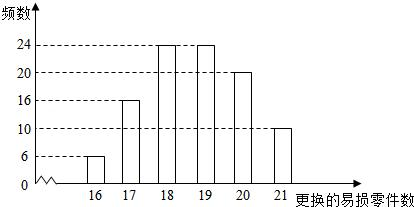
\includegraphics[width=.42\linewidth]{assets/asset-017-01.jpg}
\end{center}
\begin{solution}
\textbf{答案：}（Ⅰ）$y=\begin{cases} 200\times19=3800, & x\le19 \\ 200\times19+500(x-19)=500x-5700, & x>19 \end{cases}$；（Ⅱ）$n$的最小值为19；（Ⅲ）应购买19个易损零件。

\textbf{分析：}（Ⅰ）若$n=19$，结合题意，可得$y$与$x$的分段函数解析式；
（Ⅱ）由柱状图分别求出各组的频率，结合“需更换的易损零件数不大于$n$”的频率不小于0.5，可得$n$的最小值；
（Ⅲ）分别求出每台都购买19个易损零件，或每台都购买20个易损零件时的平均费用，比较后，可得答案。

\textbf{详解：}（Ⅰ）当$n=19$时，$y=\begin{cases} 200\times19=3800, & x\le19 \\ 200\times19+500(x-19)=500x-5700, & x>19 \end{cases}$。
（Ⅱ）由柱状图知，更换的易损零件数为16个频率为0.06，17个频率为0.16，18个频率为0.24，19个频率为0.24，又$\because$更换易损零件不大于$n$的频率为不小于0.5，$\therefore n\ge19$，$\therefore n$的最小值为19件。
（Ⅲ）假设这100台机器在购机的同时每台都购买19个易损零件，所须费用平均数为：$\frac{1}{100}(70\times19\times200+20\times(19\times200+500\times1)+10\times(19\times200+500\times2))=4000$（元）。假设这100台机器在购机的同时每台都购买20个易损零件，所须费用平均数为$\frac{1}{100}(90\times20\times200+10\times(20\times200+500\times1))=4050$（元）。$\because 4000<4050$，$\therefore$购买1台机器的同时应购买19个易损零件。
\end{solution}
\end{question}

\section*{2017 年}

\begin{question}[points=5]
\textbf{来源：}2017 年 全国III卷-理科，第 3 题\par
某城市为了解游客人数的变化规律，提高旅游服务质量，收集并整理了2014年1月至2016年12月期间月接待游客量（单位：万人）的数据，绘制了下面的折线图。根据该折线图，下列结论错误的是（ ）

\begin{center}
  
\includegraphics[width=.42\linewidth]{assets/asset-018-01.jpg}
\end{center}
\begin{choices}
  \item $A$．月接待游客量逐月增加
  \item $B$．年接待游客量逐年增加
  \item $C$．各年的月接待游客量高峰期大致在7，8月
  \item $D$．各年1月至6月的月接待游客量相对于7月至12月，波动性更小，变化比较平稳
\end{choices}
\begin{solution}
\textbf{答案：}$A$

\textbf{分析：}根据已知中2014年1月至2016年12月期间月接待游客量（单位：万人）的数据，逐一分析给定四个结论的正误，可得答案。

\textbf{详解：}由已有中2014年1月至2016年12月期间月接待游客量（单位：万人）的数据可得：月接待游客量逐月有增有减，故A错误；年接待游客量逐年增加，故B正确；各年的月接待游客量高峰期大致在7，8月，故C正确；各年1月至6月的月接待游客量相对于7月至12月，波动性更小，变化比较平稳，故D正确。故选A。
\end{solution}
\end{question}

\begin{question}[points=5]
\textbf{来源：}2017 年 全国III卷-理科，第 7 题\par
执行如图的程序框图，为使输出$S$的值小于$91$，则输入的正整数$N$的最小值为（ ）

\begin{center}
  
\includegraphics[width=.42\linewidth]{assets/asset-019-01.jpg}
\end{center}
\begin{choices}
  \item $5$
  \item $4$
  \item $3$
  \item $2$
\end{choices}
\begin{solution}
\textbf{答案：}$D$

\textbf{分析：}通过模拟程序，可得到S的取值情况，进而可得结论。

\textbf{详解：}由题可知初始值$t=1$，$M=100$，$S=0$，要使输出$S$的值小于$91$，应满足“$t\le N$”，则进入循环体，从而$S=100$，$M=-10$，$t=2$，要使输出$S$的值小于$91$，应接着满足“$t\le N$”，则进入循环体，从而$S=90$，$M=1$，$t=3$，要使输出$S$的值小于$91$，应不满足“$t\le N$”，跳出循环体，此时$N$的最小值为$2$。故选D。
\end{solution}
\end{question}

\begin{question}[points=12]
\textbf{来源：}2017 年 全国III卷-理科，第 18 题\par
某超市计划按月订购一种酸奶，每天进货量相同，进货成本每瓶4元，售价每瓶6元，未售出的酸奶降价处理，以每瓶2元的价格当天全部处理完．根据往年销售经验，每天需求量与当天最高气温（单位：℃）有关．如果最高气温不低于25，需求量为500瓶；如果最高气温位于区间[20，25），需求量为300瓶；如果最高气温低于20，需求量为200瓶．为了确定六月份的订购计划，统计了前三年六月份各天的最高气温数据，得下面的频数分布表：



| 最高气温 | [10，15) | [15，20) | [20，25) | [25，30) | [30，35) | [35，40) |

|----------|----------|----------|----------|----------|----------|----------|

| 天数     | 2        | 16       | 36       | 25       | 7        | 4        |



以最高气温位于各区间的频率代替最高气温位于该区间的概率．

（1）求六月份这种酸奶一天的需求量$X$（单位：瓶）的分布列；

（2）设六月份一天销售这种酸奶的利润为$Y$（单位：元），当六月份这种酸奶一天的进货量$n$（单位：瓶）为多少时，$Y$的数学期望达到最大值？
\begin{solution}
\textbf{答案：}（1）分布列见解析；（2）$n=300$时，$EY$最大值为$520$元

\textbf{分析：}（1）由题意知$X$的可能取值为200，300，500，分别求出相应的概率，由此能求出$X$的分布列。（2）由题意知这种酸奶一天的需求量至多为500瓶，至少为200瓶，只需考虑$200\le n\le 500$，根据$300\le n\le 500$和$200\le n\le 300$分类讨论经，能得到当$n=300$时，$EY$最大值为520元。

\textbf{详解：}解：（1）由题意知$X$的可能取值为200，300，500，$P(X=200)=\frac{2+16}{90}=0.2$，$P(X=300)=\frac{36}{90}=0.4$，$P(X=500)=\frac{25+7+4}{90}=0.4$，所以$X$的分布列为：

| $X$ | 200 | 300 | 500 |
|-----|-----|-----|-----|
| $P$ | 0.2 | 0.4 | 0.4 |

（2）由题意知这种酸奶一天的需求量至多为500瓶，至少为200瓶，所以只需考虑$200\le n\le 500$，当$300\le n\le 500$时，若最高气温不低于25，则$Y=6n-4n=2n$；若最高气温位于区间[20，25），则$Y=6\times300+2(n-300)-4n=1200-2n$；若最高气温低于20，则$Y=6\times200+2(n-200)-4n=800-2n$，所以$EY=2n\times0.4+(1200-2n)\times0.4+(800-2n)\times0.2=640-0.4n$，当$200\le n\le 300$时，若最高气温不低于20，则$Y=6n-4n=2n$，若最高气温低于20，则$Y=6\times200+2(n-200)-4n=800-2n$，所以$EY=2n\times(0.4+0.4)+(800-2n)\times0.2=160+1.2n$．所以$n=300$时，$Y$的数学期望达到最大值，最大值为520元。
\end{solution}
\end{question}

\begin{question}[points=5]
\textbf{来源：}2017 年 全国III卷-文科，第 3 题\par
某城市为了解游客人数的变化规律，提高旅游服务质量，收集并整理了2014年1月至2016年12月期间月接待游客量（单位：万人）的数据，绘制了下面的折线图。根据该折线图，下列结论错误的是（             ）

\begin{center}
  
\includegraphics[width=.42\linewidth]{assets/asset-021-01.jpg}
\end{center}
\begin{choices}
  \item A．月接待游客量逐月增加
  \item B．年接待游客量逐年增加
  \item C．各年的月接待游客量高峰期大致在7，8月
  \item D．各年1月至6月的月接待游客量相对于7月至12月，波动性更小，变化比较平稳
\end{choices}
\begin{solution}
\textbf{答案：}A

\textbf{分析：}根据已知中2014年1月至2016年12月期间月接待游客量（单位：万人）的数据，逐一分析给定四个结论的正误，可得答案。

\textbf{详解：}月接待游客量逐月有增有减，故A错误。
\end{solution}
\end{question}

\begin{question}[points=5]
\textbf{来源：}2017 年 全国III卷-文科，第 8 题\par
执行如图的程序框图，为使输出$S$的值小于$91$，则输入的正整数$N$的最小值为（       ）

\begin{center}
  
\includegraphics[width=.42\linewidth]{assets/asset-022-01.jpg}
\end{center}
\begin{choices}
  \item A．$5$
  \item B．$4$
  \item C．$3$
  \item D．$2$
\end{choices}
\begin{solution}
\textbf{答案：}D

\textbf{分析：}通过模拟程序，可得到$S$的取值情况，进而可得结论。

\textbf{详解：}初始值$t=1,M=100,S=0$，进入循环：$S=100,M=-10,t=2$；再次进入：$S=90,M=1,t=3$；此时$N$最小为$2$时跳出循环。
\end{solution}
\end{question}

\begin{question}[points=12]
\textbf{来源：}2017 年 全国III卷-文科，第 18 题\par
某超市计划按月订购一种酸奶，每天进货量相同，进货成本每瓶4元，售价每瓶6元，未售出的酸奶降价处理，以每瓶2元的价格当天全部处理完。根据往年销售经验，每天需求量与当天最高气温（单位：℃）有关。如果最高气温不低于25，需求量为500瓶；如果最高气温位于区间[20,25)，需求量为300瓶；如果最高气温低于20，需求量为200瓶。为了确定六月份的订购计划，统计了前三年六月份各天的最高气温数据，得下面的频数分布表：



最高气温  [10,15)  [15,20)  [20,25)  [25,30)  [30,35)  [35,40)

天数       2        16       36       25       7        4



以最高气温位于各区间的频率估计最高气温位于该区间的概率。

（1）求六月份这种酸奶一天的需求量不超过300瓶的概率；

（2）设六月份一天销售这种酸奶的利润为Y（单位：元），当六月份这种酸奶一天的进货量为450瓶时，写出Y的所有可能值，并估计Y大于零的概率。
\begin{solution}
\textbf{答案：}（1）$\frac{3}{5}$；（2）Y的可能值为900,300,-100；$Y>0$的概率为$\frac{4}{5}$

\textbf{分析：}（1）由前三年六月份各天的最高气温数据，求出最高气温位于区间[20,25)和最高气温低于20的天数，由此能求出六月份这种酸奶一天的需求量不超过300瓶的概率。（2）当温度大于等于25°C时，需求量为500，求出Y=900元；当温度在[20,25)°C时，需求量为300，求出Y=300元；当温度低于20°C时，需求量为200，求出Y=-100元，从而当温度大于等于20时，Y>0，由此能估计估计Y大于零的概率。

\textbf{详解：}（1）需求量不超过300瓶即最高气温低于25，天数为2+16+36=54，总天数为90，概率$p=\frac{54}{90}=\frac{3}{5}$。
（2）当最高气温≥25时，需求500，利润$Y=450\times2=900$；当20≤气温<25时，需求300，利润$Y=300\times2-150\times2=300$；当气温<20时，需求200，利润$Y=200\times6-450\times4+(450-200)\times2=-100$（按成本收入计算）。$Y>0$对应最高气温≥20，天数为90-2-16=72，概率$P=\frac{72}{90}=\frac{4}{5}$。
\end{solution}
\end{question}

\begin{question}[points=5]
\textbf{来源：}2017 年 全国II卷-理科，第 7 题\par
甲、乙、丙、丁四位同学一起去问老师询问成语竞赛的成绩．老师说：你们四人中有 $2$ 位优秀，$2$ 位良好，我现在给甲看乙、丙的成绩，给乙看丙的成绩，给丁看甲的成绩．看后甲对大家说：我还是不知道我的成绩．根据以上信息，则（   ）
\begin{choices}
  \item 乙可以知道四人的成绩
  \item 丁可以知道四人的成绩
  \item 乙、丁可以知道对方的成绩
  \item 乙、丁可以知道自己的成绩
\end{choices}
\begin{solution}
\textbf{答案：}$D$

\textbf{分析：}根据四人所知只有自己看到，老师所说及最后甲说话，继而可以推出正确答案。

\textbf{详解：}四人所知只有自己看到，老师所说及最后甲说话，甲不知自己的成绩$\rightarrow$乙丙必有一优一良，（若为两优，甲会知道自己的成绩；若是两良，甲也会知道自己的成绩）$\rightarrow$乙看到了丙的成绩，知自己的成绩$\rightarrow$丁看到甲、丁也为一优一良，丁知自己的成绩，给甲看乙丙成绩，甲不知道自已的成绩，说明乙丙一优一良，假定乙丙都是优，则甲是良，假定乙丙都是良，则甲是优，那么甲就知道自已的成绩了．给乙看丙成绩，乙没有说不知道自已的成绩，假定丙是优，则乙是良，乙就知道自己成绩．给丁看甲成绩，因为甲不知道自己成绩，乙丙是一优一良，则甲丁也是一优一良，丁看到甲成绩，假定甲是优，则丁是良，丁肯定知道自已的成绩了．故选：$D$。
\end{solution}
\end{question}

\begin{question}[points=5]
\textbf{来源：}2017 年 全国II卷-理科，第 8 题\par
执行如图的程序框图，如果输入的 $a=-1$，则输出的 $S=$（   ）

\begin{center}
  
\includegraphics[width=.42\linewidth]{assets/asset-025-01.jpg}
\end{center}
\begin{choices}
  \item $2$
  \item $3$
  \item $4$
  \item $5$
\end{choices}
\begin{solution}
\textbf{答案：}$B$

\textbf{分析：}执行程序框图，依次写出每次循环得到的 $S$，$K$ 值，当 $K=7$ 时，程序终止即可得到结论。

\textbf{详解：}执行程序框图，有 $S=0$，$K=1$，$a=-1$，代入循环，第一次满足循环，$S=-1$，$a=1$，$K=2$；满足条件，第二次满足循环，$S=1$，$a=-1$，$K=3$；满足条件，第三次满足循环，$S=-2$，$a=1$，$K=4$；满足条件，第四次满足循环，$S=2$，$a=-1$，$K=5$；满足条件，第五次满足循环，$S=-3$，$a=1$，$K=6$；满足条件，第六次满足循环，$S=3$，$a=-1$，$K=7$；$K\le 6$ 不成立，退出循环输出 $S$ 的值为 $3$．故选：$B$。
\end{solution}
\end{question}

\begin{question}[points=5]
\textbf{来源：}2017 年 全国II卷-理科，第 13 题\par
一批产品的二等品率为 $0.02$，从这批产品中每次随机取一件，有放回地抽取 $100$ 次．$X$ 表示抽到的二等品件数，则 $DX=$ ．
\fillin[{$1.96$}]
\begin{solution}
\textbf{答案：}$1.96$

\textbf{分析：}判断概率满足的类型，然后求解方差即可。

\textbf{详解：}由题意可知，该事件满足独立重复试验，是一个二项分布模型，其中，$p=0.02$，$n=100$，则 $DX=npq=np(1-p)=100\times0.02\times0.98=1.96$．故答案为：$1.96$。
\end{solution}
\end{question}

\begin{question}[points=12]
\textbf{来源：}2017 年 全国II卷-理科，第 18 题\par
海水养殖场进行某水产品的新、旧网箱养殖方法的产量对比，收获时各随机抽取了 $100$ 个网箱，测量各箱水产品的产量（单位：kg），其频率分布直方图如图：

（1）设两种养殖方法的箱产量相互独立，记 $A$ 表示事件“旧养殖法的箱产量低于 $50$kg，新养殖法的箱产量不低于 $50$kg”，估计 $A$ 的概率；

（2）填写下面列联表，并根据列联表判断是否有 $99\%$ 的把握认为箱产量与养殖方法有关：

$\begin{array}{c|cc} & \text{箱产量}<50\text{kg} & \text{箱产量}\ge50\text{kg} \\ \hline \text{旧养殖法} & & \\ \text{新养殖法} & & \end{array}$

（3）根据箱产量的频率分布直方图，求新养殖法箱产量的中位数的估计值（精确到 $0.01$）．

附：$P(K^2\ge k)$ 的临界值表：$k_{0.050}=3.841$，$k_{0.010}=6.635$，$k_{0.001}=10.828$，$K^2=\frac{n(ad-bc)^2}{(a+b)(c+d)(a+c)(b+d)}$．

\begin{center}
  
\includegraphics[width=.42\linewidth]{assets/asset-027-01.jpg}
\end{center}
\begin{solution}
\textbf{答案：}（1）$0.4092$；（2）有 $99\%$ 的把握认为箱产量与养殖方法有关；（3）$52.35$kg

\textbf{分析：}（1）由题意可知：$P(A)=P(BC)=P(B)P(C)$，分布求得发生的频率，即可求得其概率；（2）完成 $2\times2$ 列联表：求得观测值，与参考值比较，即可求得有 $99\%$ 的把握认为箱产量与养殖方法有关：（3）根据频率分布直方图即可求得其中位数。

\textbf{详解：}（1）记 $B$ 表示事件“旧养殖法的箱产量低于 $50$kg”，$C$ 表示事件“新养殖法的箱产量不低于 $50$kg”，由 $P(A)=P(BC)=P(B)P(C)$，则旧养殖法的箱产量低于 $50$kg：$(0.012+0.014+0.024+0.034+0.040)\times5=0.62$，故 $P(B)$ 的估计值 $0.62$，新养殖法的箱产量不低于 $50$kg：$(0.068+0.046+0.010+0.008)\times5=0.66$，故 $P(C)$ 的估计值为 $0.66$，则事件 $A$ 的概率估计值为 $P(A)=P(B)P(C)=0.62\times0.66=0.4092$；
（2）$2\times2$ 列联表：
$\begin{array}{c|cc|c} & \text{箱产量}<50\text{kg} & \text{箱产量}\ge50\text{kg} & \text{总计} \\ \hline \text{旧养殖法} & 62 & 38 & 100 \\ \text{新养殖法} & 34 & 66 & 100 \\ \hline \text{总计} & 96 & 104 & 200 \end{array}$
则 $K^2=\frac{200\times(62\times66-38\times34)^2}{100\times100\times96\times104}\approx15.705$，由 $15.705>6.635$，$\therefore$ 有 $99\%$ 的把握认为箱产量与养殖方法有关；
（3）由新养殖法的箱产量频率分布直方图中，箱产量低于 $50$kg 的直方图的面积：$(0.004+0.020+0.044)\times5=0.34$，箱产量低于 $55$kg 的直方图面积为：$(0.004+0.020+0.044+0.068)\times5=0.68>0.5$，故新养殖法产量的中位数的估计值为：$50+\frac{0.5-0.34}{0.068}\approx52.35$（kg），新养殖法箱产量的中位数的估计值 $52.35$（kg）。
\end{solution}
\end{question}

\begin{question}[points=5]
\textbf{来源：}2017 年 全国II卷-文科，第 9 题\par
甲、乙、丙、丁四位同学一起去问老师询问成语竞赛的成绩. 老师说: 你们四人中有2位优秀, 2位良好, 我现在给甲看乙、丙的成绩, 给乙看丙的成绩, 给丁看甲的成绩. 看后甲对大家说: 我还是不知道我的成绩. 根据以上信息, 则
\begin{choices}
  \item 乙可以知道四人的成绩
  \item 丁可以知道四人的成绩
  \item 乙、丁可以知道对方的成绩
  \item 乙、丁可以知道自己的成绩
\end{choices}
\begin{solution}
\textbf{答案：}乙、丁可以知道自己的成绩

\textbf{分析：}根据四人所知只有自己看到, 老师所说及最后甲说话, 继而可以推出正确答案.

\textbf{详解：}四人所知只有自己看到, 老师所说及最后甲说话, 甲不知自己的成绩 $\rightarrow$ 乙丙必有一优一良, (若为两优, 甲会知道自己的成绩; 若是两良, 甲也会知道自己的成绩) $\rightarrow$ 乙看到了丙的成绩, 知自己的成绩 $\rightarrow$ 丁看到甲、丁也为一优一良, 丁知自己的成绩, 给甲看乙丙成绩, 甲不知道自已的成绩, 说明乙丙一优一良, 假定乙丙都是优, 则甲是良, 假定乙丙都是良, 则甲是优, 那么甲就知道自已的成绩了. 给乙看丙成绩, 乙没有说不知道自已的成绩, 假定丙是优, 则乙是良, 乙就知道自己成绩. 给丁看甲成绩, 因为甲不知道自己成绩, 乙丙是一优一良, 则甲丁也是一优一良, 丁看到甲成绩, 假定甲是优, 则丁是良, 丁肯定知道自已的成绩了. 故选D.
\end{solution}
\end{question}

\begin{question}[points=5]
\textbf{来源：}2017 年 全国II卷-文科，第 10 题\par
执行如图的程序框图, 如果输入的 $a=-1$, 则输出的 $S=$

\begin{center}
  
\includegraphics[width=.42\linewidth]{assets/asset-029-01.jpg}
\end{center}
\begin{choices}
  \item $2$
  \item $3$
  \item $4$
  \item $5$
\end{choices}
\begin{solution}
\textbf{答案：}$3$

\textbf{分析：}执行程序框图, 依次写出每次循环得到的 $S$, $K$ 值, 当 $K=7$ 时, 程序终止即可得到结论.

\textbf{详解：}执行程序框图, 有 $S=0$, $K=1$, $a=-1$, 代入循环, 第一次满足循环, $S=-1$, $a=1$, $K=2$; 满足条件, 第二次满足循环, $S=1$, $a=-1$, $K=3$; 满足条件, 第三次满足循环, $S=-2$, $a=1$, $K=4$; 满足条件, 第四次满足循环, $S=2$, $a=-1$, $K=5$; 满足条件, 第五次满足循环, $S=-3$, $a=1$, $K=6$; 满足条件, 第六次满足循环, $S=3$, $a=-1$, $K=7$; $K\le 6$ 不成立, 退出循环输出 $S$ 的值为 $3$. 故选B.
\end{solution}
\end{question}

\begin{question}[points=5]
\textbf{来源：}2017 年 全国II卷-文科，第 11 题\par
从分别写有 $1,2,3,4,5$ 的 $5$ 张卡片中随机抽取 $1$ 张, 放回后再随机抽取 $1$ 张, 则抽得的第一张卡片上的数大于第二张卡片上的数的概率为
\begin{choices}
  \item $\frac{1}{10}$
  \item $\frac{1}{5}$
  \item $\frac{3}{10}$
  \item $\frac{2}{5}$
\end{choices}
\begin{solution}
\textbf{答案：}$\frac{2}{5}$

\textbf{分析：}先求出基本事件总数 $n=5\times5=25$, 再用列举法求出抽得的第一张卡片上的数大于第二张卡片上的数包含的基本事件个数, 由此能求出概率.

\textbf{详解：}基本事件总数 $n=5\times5=25$, 抽得的第一张卡片上的数大于第二张卡片上的数包含的基本事件有: $(2,1),(3,1),(3,2),(4,1),(4,2),(4,3),(5,1),(5,2),(5,3),(5,4)$, 共有 $m=10$ 个基本事件, $\therefore$ 抽得的第一张卡片上的数大于第二张卡片上的数的概率 $p=\frac{m}{n}=\frac{10}{25}=\frac{2}{5}$. 故选D.
\end{solution}
\end{question}

\begin{question}[points=12]
\textbf{来源：}2017 年 全国II卷-文科，第 19 题\par
海水养殖场进行某水产品的新、旧网箱养殖方法的产量对比, 收获时各随机抽取了100个网箱, 测量各箱水产品的产量 (单位: kg), 其频率分布直方图如下: \\ (1) 记 $A$ 表示事件“旧养殖法的箱产量低于$50\text{kg}$”, 估计 $A$ 的概率; \\ (2) 填写下面列联表, 并根据列联表判断是否有$99\%$的把握认为箱产量与养殖方法有关; \\ (3) 根据箱产量的频率分布直方图, 对两种养殖方法的优劣进行比较. \\ 附: $P(K^2\ge k)$ $0.050$ $0.010$ $0.001$; $k$ $3.841$ $6.635$ $10.828$; $K^2=\frac{n(ad-bc)^2}{(a+b)(c+d)(a+c)(b+d)}$.

\begin{center}
  
\includegraphics[width=.42\linewidth]{assets/asset-031-01.jpg}
\end{center}
\begin{solution}

\textbf{分析：}(1) 根据题意, 由旧养殖法的频率分布直方图计算可得答案; (2) 由频率分布直方图可以将列联表补全, 进而计算可得 $K^2\approx15.705>6.635$, 与附表比较即可得答案; (3) 由频率分布直方图计算新旧养殖法产量的平均数, 比较即可得答案.

\textbf{详解：}(1) 根据题意, 由旧养殖法的频率分布直方图可得: $P(A)=(0.012+0.014+0.024+0.034+0.040)\times5=0.62$; \\ (2) 根据题意, 补全列联表可得: $\begin{array}{c|ccc} & \text{箱产量}<50\text{kg} & \text{箱产量}\ge50\text{kg} & \text{总计} \\ \hline \text{旧养殖法} & 62 & 38 & 100 \\ \text{新养殖法} & 34 & 66 & 100 \\ \text{总计} & 96 & 104 & 200 \end{array}$ 则有 $K^2=\frac{200\times(62\times66-38\times34)^2}{100\times100\times96\times104}\approx15.705>6.635$, 故有 $99\%$ 的把握认为箱产量与养殖方法有关; \\ (3) 由频率分布直方图可得: 旧养殖法100个网箱产量的平均数 $\bar{x}_1=(27.5\times0.012+32.5\times0.014+37.5\times0.024+42.5\times0.034+47.5\times0.040+52.5\times0.032+57.5\times0.032+62.5\times0.012+67.5\times0.012)\times5=5\times9.42=47.1$; 新养殖法100个网箱产量的平均数 $\bar{x}_2=(37.5\times0.004+42.5\times0.020+47.5\times0.044+52.5\times0.054+57.5\times0.046+62.5\times0.010+67.5\times0.008)\times5=5\times10.47=52.35$; 比较可得 $\bar{x}_1<\bar{x}_2$, 故新养殖法更加优于旧养殖法.
\end{solution}
\end{question}

\begin{question}[points=5]
\textbf{来源：}2017 年 全国I卷-理科，第 2 题\par
如图，正方形 $ABCD$ 内的图形来自中国古代的太极图．正方形内切圆中的黑色部分和白色部分关于正方形的中心成中心对称．在正方形内随机取一点，则此点取自黑色部分的概率是（ ）

\begin{center}
  
\includegraphics[width=.42\linewidth]{assets/asset-032-01.jpg}
\end{center}
\begin{choices}
  \item $\frac{1}{4}$
  \item $\frac{\pi}{8}$
  \item $\frac{1}{2}$
  \item $\frac{\pi}{4}$
\end{choices}
\begin{solution}
\textbf{答案：}B

\textbf{分析：}根据图象的对称性求出黑色图形的面积，结合几何概型的概率公式进行求解即可．

\textbf{详解：}根据图象的对称性知，黑色部分为圆面积的一半，设圆的半径为 1，则正方形的边长为 2，则黑色部分的面积 $S=\frac{\pi}{2}$，则对应概率 $P=\frac{\pi/2}{4}=\frac{\pi}{8}$．故选：B．
\end{solution}
\end{question}

\begin{question}[points=5]
\textbf{来源：}2017 年 全国I卷-理科，第 8 题\par
如图程序框图是为了求出满足 $3^n-2^n>1000$ 的最小偶数 $n$，那么在 $\boxed{}$ 和 $\boxed{}$ 两个空白框中，可以分别填入（ ）

\begin{center}
  
\includegraphics[width=.42\linewidth]{assets/asset-033-01.jpg}
\end{center}
\begin{choices}
  \item $A>1000$ 和 $n=n+1$
  \item $A>1000$ 和 $n=n+2$
  \item $A\leq 1000$ 和 $n=n+1$
  \item $A\leq 1000$ 和 $n=n+2$
\end{choices}
\begin{solution}
\textbf{答案：}D

\textbf{分析：}通过要求 $A>1000$ 时输出且框图中在“否”时输出确定“$\boxed{}$”内不能输入“$A>1000$”，进而通过偶数的特征确定 $n=n+2$．

\textbf{详解：}因为要求 $A>1000$ 时输出，且框图中在“否”时输出，所以“$\boxed{}$”内不能输入“$A>1000$”，又要求 $n$ 为偶数，且 $n$ 的初始值为 0，所以“$\boxed{}$”中 $n$ 依次加 2 可保证其为偶数，所以 D 选项满足要求．故选：D．
\end{solution}
\end{question}

\begin{question}[points=12]
\textbf{来源：}2017 年 全国I卷-理科，第 19 题\par
为了监控某种零件的一条生产线的生产过程，检验员每天从该生产线上随机抽取 16 个零件，并测量其尺寸（单位：cm）．根据长期生产经验，可以认为这条生产线正常状态下生产的零件的尺寸服从正态分布 $N(\mu,\sigma^2)$．

（1）假设生产状态正常，记 $X$ 表示一天内抽取的 16 个零件中其尺寸在 $(\mu-3\sigma,\mu+3\sigma)$ 之外的零件数，求 $P(X\geq 1)$ 及 $X$ 的数学期望；

（2）一天内抽检零件中，如果出现了尺寸在 $(\mu-3\sigma,\mu+3\sigma)$ 之外的零件，就认为这条生产线在这一天的生产过程可能出现了异常情况，需对当天的生产过程进行检查．

（$\text{i}$）试说明上述监控生产过程方法的合理性；

（$\text{ii}$）下面是检验员在一天内抽取的 16 个零件的尺寸：



$9.95\quad 10.12\quad 9.96\quad 9.96\quad 10.01\quad 9.92\quad 9.98\quad 10.04$



$10.26\quad 9.91\quad 10.13\quad 10.02\quad 9.22\quad 10.04\quad 10.05\quad 9.95$



经计算得 $\bar{x}=\frac{1}{16}\sum_{i=1}^{16}x_i=9.97$，$s=\sqrt{\frac{1}{16}\sum_{i=1}^{16}(x_i-\bar{x})^2}=\sqrt{\frac{1}{16}(\sum_{i=1}^{16}x_i^2-16\bar{x}^2)}\approx0.212$，

其中 $x_i$ 为抽取的第 $i$ 个零件的尺寸，$i=1,2,\ldots,16$．



用样本平均数 $\bar{x}$ 作为 $\mu$ 的估计值 $\hat{\mu}$，用样本标准差 $s$ 作为 $\sigma$ 的估计值 $\hat{\sigma}$，利用估计值判断是否需对当天的生产过程进行检查？剔除 $(\hat{\mu}-3\hat{\sigma},\hat{\mu}+3\hat{\sigma})$ 之外的数据，用剩下的数据估计 $\mu$ 和 $\sigma$（精确到 0.01）．

附：若随机变量 $Z$ 服从正态分布 $N(\mu,\sigma^2)$，则 $P(\mu-3\sigma<Z<\mu+3\sigma)=0.9974$，$0.9974^{16}\approx0.9592$，$\sqrt{0.008}\approx0.09$．
\begin{solution}
\textbf{答案：}（1）$P(X\geq1)=0.0408$，$E(X)=0.0416$；（2）（$\text{i}$）见解析；（$\text{ii}$）需检查，$\mu$ 的估计值为 $10.02$，$\sigma$ 的估计值为 $0.09$

\textbf{分析：}（1）通过 $P(X=0)$ 可求出 $P(X\geq1)=1-P(X=0)=0.0408$，利用二项分布的期望公式计算可得结论；（2）（$\text{i}$）由（1）及知落在 $(\mu-3\sigma,\mu+3\sigma)$ 之外为小概率事件可知该监控生产过程方法合理；（$\text{ii}$）通过样本平均数 $\bar{x}$、样本标准差 $s$ 估计 $\hat{\mu}$、$\hat{\sigma}$ 可知 $(\hat{\mu}-3\hat{\sigma},\hat{\mu}+3\hat{\sigma})=(9.334,10.606)$，进而需剔除 $(\hat{\mu}-3\hat{\sigma},\hat{\mu}+3\hat{\sigma})$ 之外的数据 $9.22$，利用公式计算即得结论．

\textbf{详解：}解：（1）由题可知尺寸落在 $(\mu-3\sigma,\mu+3\sigma)$ 之内的概率为 $0.9974$，则落在 $(\mu-3\sigma,\mu+3\sigma)$ 之外的概率为 $1-0.9974=0.0026$，因为 $P(X=0)=C_{16}^0\times(1-0.9974)^0\times0.9974^{16}\approx0.9592$，所以 $P(X\geq1)=1-P(X=0)=0.0408$，又因为 $X\sim B(16,0.0026)$，所以 $E(X)=16\times0.0026=0.0416$．
（2）（$\text{i}$）如果生产状态正常，一个零件尺寸在 $(\hat{\mu}-3\hat{\sigma},\hat{\mu}+3\hat{\sigma})$ 之外的概率只有 $0.0026$，一天内抽取的 16 个零件中，出现尺寸在 $(\hat{\mu}-3\hat{\sigma},\hat{\mu}+3\hat{\sigma})$ 之外的零件的概率只有 $0.0408$，发生的概率很小．因此一旦发生这种状况，就有理由认为这条生产线在这一天的生产过程可能出现了异常情况，需对当天的生产过程进行检查，可见上述监控生产过程的方法是合理的．
（$\text{ii}$）由 $\bar{x}=9.97$，$s\approx0.212$，得 $\mu$ 的估计值为 $\hat{\mu}=9.97$，$\sigma$ 的估计值为 $\hat{\sigma}=0.212$，由样本数据可以看出一个零件的尺寸在 $(\hat{\mu}-3\hat{\sigma},\hat{\mu}+3\hat{\sigma})$ 之外，因此需对当天的生产过程进行检查．剔除 $(\hat{\mu}-3\hat{\sigma},\hat{\mu}+3\hat{\sigma})$ 之外的数据 $9.22$，剩下的数据的平均数为 $\frac{1}{15}(16\times9.97-9.22)=10.02$，因此 $\mu$ 的估计值为 $10.02$．$\sum_{i=1}^{16}x_i^2=16\times0.212^2+16\times9.97^2\approx1591.134$，剔除 $(\hat{\mu}-3\hat{\sigma},\hat{\mu}+3\hat{\sigma})$ 之外的数据 $9.22$，剩下的数据的样本方差为 $\frac{1}{15}(1591.134-9.22^2-15\times10.02^2)\approx0.008$，因此 $\sigma$ 的估计值为 $\sqrt{0.008}\approx0.09$．
\end{solution}
\end{question}

\begin{question}[points=5]
\textbf{来源：}2017 年 全国I卷-文科，第 2 题\par
为评估一种农作物的种植效果，选了$n$块地作试验田．这$n$块地的亩产量（单位：$\text{kg}$）分别是$x_1$，$x_2$，$\ldots$，$x_n$，下面给出的指标中可以用来评估这种农作物亩产量稳定程度的是（           ）
\begin{choices}
  \item $x_1$，$x_2$，$\ldots$，$x_n$的平均数
  \item $x_1$，$x_2$，$\ldots$，$x_n$的标准差
  \item $x_1$，$x_2$，$\ldots$，$x_n$的最大值
  \item $x_1$，$x_2$，$\ldots$，$x_n$的中位数
\end{choices}
\begin{solution}
\textbf{答案：}B

\textbf{分析：}利用平均数、标准差、最大值、中位数的定义和意义直接求解。

\textbf{详解：}解：在A中，平均数是表示一组数据集中趋势的量数，它是反映数据集中趋势的一项指标，故A不可以用来评估这种农作物亩产量稳定程度；在B中，标准差能反映一个数据集的离散程度，故B可以用来评估这种农作物亩产量稳定程度；在C中，最大值是一组数据最大的量，故C不可以用来评估这种农作物亩产量稳定程度；在D中，中位数将数据分成前半部分和后半部分，用来代表一组数据的“中等水平”，故D不可以用来评估这种农作物亩产量稳定程度。故选：B。
\end{solution}
\end{question}

\begin{question}[points=5]
\textbf{来源：}2017 年 全国I卷-文科，第 4 题\par
如图，正方形$ABCD$内的图形来自中国古代的太极图．正方形内切圆中的黑色部分和白色部分关于正方形的中心成中心对称．在正方形内随机取一点，则此点取自黑色部分的概率是（                 ）

\begin{center}
  
\includegraphics[width=.42\linewidth]{assets/asset-036-01.jpg}
\end{center}
\begin{choices}
  \item $\frac{1}{4}$
  \item $\frac{1}{8}$
  \item $\frac{1}{2}$
  \item $\frac{\pi}{4}$
\end{choices}
\begin{solution}
\textbf{答案：}B

\textbf{分析：}根据图象的对称性求出黑色图形的面积，结合几何概型的概率公式进行求解即可。

\textbf{详解：}解：根据图象的对称性知，黑色部分为圆面积的一半，设圆的半径为1，则正方形的边长为2，则黑色部分的面积$S=\frac{\pi}{2}$，则对应概率$P=\frac{\frac{\pi}{2}}{4}=\frac{\pi}{8}$，故选：B。
\end{solution}
\end{question}

\begin{question}[points=5]
\textbf{来源：}2017 年 全国I卷-文科，第 10 题\par
如图程序框图是为了求出满足$3^n-2^n>1000$的最小偶数$n$，那么在$\boxed{}$和$\boxed{}$两个空白框中，可以分别填入（             ）

\begin{center}
  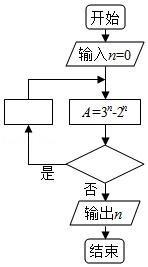
\includegraphics[width=.42\linewidth]{assets/asset-037-01.jpg}
\end{center}
\begin{choices}
  \item $A>1000$和$n=n+1$
  \item $A>1000$和$n=n+2$
  \item $A\le 1000$和$n=n+1$
  \item $A\le 1000$和$n=n+2$
\end{choices}
\begin{solution}
\textbf{答案：}D

\textbf{分析：}通过要求$A>1000$时输出且框图中在“否”时输出确定“$\boxed{}$”内不能输入“$A>1000$”，进而通过偶数的特征确定$n=n+2$。

\textbf{详解：}解：因为要求$A>1000$时输出，且框图中在“否”时输出，所以“$\boxed{}$”内不能输入“$A>1000$”，又要求$n$为偶数，且$n$的初始值为0，所以“$\boxed{}$”中$n$依次加2可保证其为偶数，所以D选项满足要求，故选：D。
\end{solution}
\end{question}

\begin{question}[points=12]
\textbf{来源：}2017 年 全国I卷-文科，第 19 题\par
为了监控某种零件的一条生产线的生产过程，检验员每隔$30\text{min}$从该生产线上随机抽取一个零件，并测量其尺寸（单位：$\text{cm}$）．下面是检验员在一天内依次抽取的$16$个零件的尺寸：



抽取次序 1 2 3 4 5 6 7 8

零件尺寸 9.95 10.12 9.96 9.96 10.01 9.92 9.98 10.04

抽取次序 9 10 11 12 13 14 15 16

零件尺寸 10.26 9.91 10.13 10.02 9.22 10.04 10.05 9.95



经计算得$\bar{x}=\frac{1}{16}\sum_{i=1}^{16}x_i=9.97$，$s=\sqrt{\frac{1}{16}\sum_{i=1}^{16}(x_i-\bar{x})^2}=\sqrt{\frac{1}{16}(\sum_{i=1}^{16}x_i^2-16\bar{x}^2)}\approx0.212$，$\sqrt{\sum_{i=1}^{16}(i-8.5)^2}\approx18.439$，$\sum_{i=1}^{16}(x_i-\bar{x})(i-8.5)=-2.78$，其中$x_i$为抽取的第$i$个零件的尺寸，$i=1,2,\ldots,16$．

（1）求$(x_i,i)$（$i=1,2,\ldots,16$）的相关系数$r$，并回答是否可以认为这一天生产的零件尺寸不随生产过程的进行而系统地变大或变小（若$|r|<0.25$，则可以认为零件的尺寸不随生产过程的进行而系统地变大或变小）．

（2）一天内抽检零件中，如果出现了尺寸在$(\bar{x}-3s,\bar{x}+3s)$之外的零件，就认为这条生产线在这一天的生产过程可能出现了异常情况，需对当天的生产过程进行检查．

（i）从这一天抽检的结果看，是否需对当天的生产过程进行检查？

（ii）在$(\bar{x}-3s,\bar{x}+3s)$之外的数据称为离群值，试剔除离群值，估计这条生产线当天生产的零件尺寸的均值与标准差．（精确到$0.01$）



附：样本$(x_i,y_i)$（$i=1,2,\ldots,n$）的相关系数$r=\frac{\sum_{i=1}^{n}(x_i-\bar{x})(y_i-\bar{y})}{\sqrt{\sum_{i=1}^{n}(x_i-\bar{x})^2}\sqrt{\sum_{i=1}^{n}(y_i-\bar{y})^2}}$，$\sqrt{0.008}\approx0.09$．

\begin{center}
  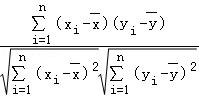
\includegraphics[width=.42\linewidth]{assets/asset-038-01.jpg}
\end{center}
\begin{solution}
\textbf{答案：}（1）$r\approx-0.18$，可以认为；（2）（i）需要对当天的生产过程进行检查；（ii）均值约为$10.02$，标准差约为$0.09$。

\textbf{分析：}（1）代入数据计算，比较$|r|$与$0.25$的大小作出结论；（2）（i）计算合格零件尺寸范围，得出结论；（ii）代入公式计算即可。

\textbf{详解：}解：（1）$r=\frac{\sum_{i=1}^{16}(x_i-\bar{x})(i-8.5)}{\sqrt{\sum_{i=1}^{16}(x_i-\bar{x})^2}\sqrt{\sum_{i=1}^{16}(i-8.5)^2}}=\frac{-2.78}{16\times0.212\times18.439}\approx-0.18$．$\because|r|<0.25$，$\therefore$可以认为这一天生产的零件尺寸不随生产过程的进行而系统地变大或变小．
（2）（i）$\bar{x}=9.97$，$s=0.212$，$\therefore$合格零件尺寸范围是$(9.334,10.606)$，显然第$13$号零件尺寸$9.22$不在此范围之内，$\therefore$需要对当天的生产过程进行检查．
（ii）剔除离群值后，剩下的数据平均值为$\frac{16\times9.97-9.22}{15}=10.02$，$\sum_{i=1}^{16}x_i^2=16\times0.212^2+16\times9.97^2=1591.134$，$\therefore$剔除离群值后样本方差为$\frac{1}{15}(1591.134-9.22^2-15\times10.02^2)=0.008$，$\therefore$剔除离群值后样本标准差为$\sqrt{0.008}\approx0.09$．
\end{solution}
\end{question}

\section*{2018 年}

\begin{question}[points=5]
\textbf{来源：}2018 年 全国III卷-理科，第 8 题\par
某群体中的每位成员使用移动支付的概率都为$p$，各成员的支付方式相互独立．设$X$为该群体的10位成员中使用移动支付的人数，$DX=2.4$，$P(X=4)<P(X=6)$，则$p=$（ ）
\begin{choices}
  \item $0.7$
  \item $0.6$
  \item $0.4$
  \item $0.3$
\end{choices}
\begin{solution}
\textbf{答案：}B

\textbf{分析：}利用已知条件，转化为二项分布，利用方差和概率大小关系求解．

\textbf{详解：}由题意$X\sim B(10,p)$，$DX=10p(1-p)=2.4$，解得$p=0.6$或$p=0.4$．由$P(X=4)<P(X=6)$，即$C_{10}^4 p^4(1-p)^6 < C_{10}^6 p^6(1-p)^4$，化简得$(1-p)^2 < p^2$，即$1-p < p$，故$p>0.5$，所以$p=0.6$．
\end{solution}
\end{question}

\begin{question}[points=12]
\textbf{来源：}2018 年 全国III卷-理科，第 18 题\par
某工厂为提高生产效率，开展技术创新活动，提出了完成某项生产任务的两种新的生产方式．为比较两种生产方式的效率，选取40名工人，将他们随机分成两组，每组20人．第一组工人用第一种生产方式，第二组工人用第二种生产方式．根据工人完成生产任务的工作时间（单位：min）绘制了如下茎叶图：



（1）根据茎叶图判断哪种生产方式的效率更高？并说明理由；

（2）求40名工人完成生产任务所需时间的中位数$m$，并将完成生产任务所需时间超过$m$和不超过$m$的工人数填入下面的列联表：



| | 超过$m$ | 不超过$m$ |

| --- | --- | --- |

| 第一种生产方式 | | |

| 第二种生产方式 | | |



（3）根据（2）中的列联表，能否有99%的把握认为两种生产方式的效率有差异？



附：$K^2=\frac{n(ad-bc)^2}{(a+b)(c+d)(a+c)(b+d)}$，



$P(K^2\geq k)$ | 0.050 | 0.010 | 0.001

--- | --- | --- | ---

$k$ | 3.841 | 6.635 | 10.828

\begin{center}
  
\includegraphics[width=.42\linewidth]{assets/asset-040-01.jpg}
\end{center}
\begin{solution}

\textbf{分析：}（1）根据茎叶图中的数据判断第二种生产方式的工作时间较少些，效率更高；（2）根据茎叶图中的数据计算它们的中位数，再填写列联表；（3）列联表中的数据计算观测值，对照临界值得出结论．

\textbf{详解：}（1）第二种生产方式效率更高，因为第二种生产方式的工作时间主要集中在65~85之间，而第一种集中在72~92之间，第二种整体工作时间更短．
（2）中位数$m=\frac{79+81}{2}=80$，列联表如下：

| | 超过$m$ | 不超过$m$ | 总计 |
| --- | --- | --- | --- |
| 第一种生产方式 | 15 | 5 | 20 |
| 第二种生产方式 | 5 | 15 | 20 |
| 总计 | 20 | 20 | 40 |

（3）$K^2=\frac{40\times(15\times15-5\times5)^2}{20\times20\times20\times20}=10>6.635$，所以有99%的把握认为两种生产方式的效率有差异．
\end{solution}
\end{question}

\begin{question}[points=5]
\textbf{来源：}2018 年 全国III卷-文科，第 5 题\par
若某群体中的成员只用现金支付的概率为 $0.45$，既用现金支付也用非现金支付的概率为 $0.15$，则不用现金支付的概率为
\begin{choices}
  \item $0.3$
  \item $0.4$
  \item $0.6$
  \item $0.7$
\end{choices}
\begin{solution}
\textbf{答案：}B

\textbf{分析：}直接利用互斥事件的概率的加法公式求解即可．

\textbf{详解：}某群体中的成员只用现金支付，既用现金支付也用非现金支付，不用现金支付，是互斥事件，所以不用现金支付的概率为：$1-0.45-0.15=0.4$．故选：B．
\end{solution}
\end{question}

\begin{question}[points=5]
\textbf{来源：}2018 年 全国III卷-文科，第 14 题\par
某公司有大量客户，且不同年龄段客户对其服务的评价有较大差异．为了解客户的评价，该公司准备进行抽样调查，可供选择的抽样方法有简单随机抽样、分层抽样和系统抽样，则最合适的抽样方法是
\fillin[{$分层抽样$}]
\begin{solution}
\textbf{答案：}$分层抽样$

\textbf{分析：}利用简单随机抽样、分层抽样和系统抽样的定义、性质直接求解．

\textbf{详解：}某公司有大量客户，且不同年龄段客户对其服务的评价有较大差异，为了解客户的评价，该公司准备进行抽样调查，可供选择的抽样方法有简单随机抽样、分层抽样和系统抽样，则最合适的抽样方法是分层抽样．故答案为：分层抽样．
\end{solution}
\end{question}

\begin{question}[points=12]
\textbf{来源：}2018 年 全国III卷-文科，第 18 题\par
某工厂为提高生产效率，开展技术创新活动，提出了完成某项生产任务的两种新的生产方式．为比较两种生产方式的效率，选取 40 名工人，将他们随机分成两组，每组 20 人．第一组工人用第一种生产方式，第二组工人用第二种生产方式．根据工人完成生产任务的工作时间（单位：min）绘制了如下茎叶图：

(1) 根据茎叶图判断哪种生产方式的效率更高？并说明理由；

(2) 求 40 名工人完成生产任务所需时间的中位数 $m$，并将完成生产任务所需时间超过 $m$ 和不超过 $m$ 的工人数填入下面的列联表：



                    超过 $m$      不超过 $m$

第一种生产方式

第二种生产方式



(3) 根据(2)中的列联表，能否有 99% 的把握认为两种生产方式的效率有差异？

附：$K^2=\frac{n(ad-bc)^2}{(a+b)(c+d)(a+c)(b+d)}$，

$P(K^2\ge k)$  0.050  0.010  0.001

$k$           3.841  6.635 10.828

\begin{center}
  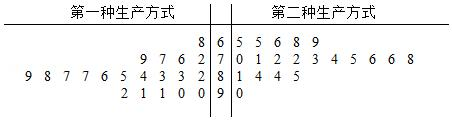
\includegraphics[width=.42\linewidth]{assets/asset-043-01.jpg}
\end{center}

\begin{center}
  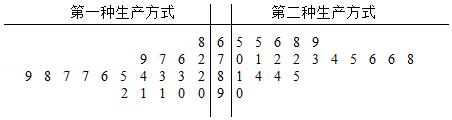
\includegraphics[width=.42\linewidth]{assets/asset-043-02.jpg}
\end{center}
\begin{solution}

\textbf{分析：}(1) 根据茎叶图中的数据判断第二种生产方式的工作时间较少些，效率更高；
(2) 根据茎叶图中的数据计算它们的中位数，再填写列联表；
(3) 列联表中的数据计算观测值，对照临界值得出结论．

\textbf{详解：}(1) 根据茎叶图中的数据知，第一种生产方式的工作时间主要集中在 72～92 之间，第二种生产方式的工作时间主要集中在 65～85 之间，所以第二种生产方式的工作时间较少些，效率更高．
(2) 这 40 名工人完成生产任务所需时间按从小到大的顺序排列后，排在中间的两个数据是 79 和 81，计算它们的中位数为 $m=\frac{79+81}{2}=80$．由此填写列联表如下：

                  超过 $m$    不超过 $m$   总计
第一种生产方式      15          5         20
第二种生产方式       5         15         20
总计               20         20         40

(3) 根据(2)中的列联表，计算 $K^2=\frac{40\times(15\times15-5\times5)^2}{20\times20\times20\times20}=\frac{40\times(225-25)^2}{160000}=\frac{40\times200^2}{160000}=10>6.635$，$\therefore$ 能有 99% 的把握认为两种生产方式的效率有差异．
\end{solution}
\end{question}

\begin{question}[points=5]
\textbf{来源：}2018 年 全国II卷-理科，第 8 题\par
我国数学家陈景润在哥德巴赫猜想的研究中取得了世界领先的成果．哥德巴赫猜想是“每个大于$2$的偶数可以表示为两个素数的和”，如$30=7+23$．在不超过$30$的素数中，随机选取两个不同的数，其和等于$30$的概率是（                   ）
\begin{choices}
  \item $\frac{1}{12}$
  \item $\frac{1}{14}$
  \item $\frac{1}{15}$
  \item $\frac{1}{18}$
\end{choices}
\begin{solution}
\textbf{答案：}C

\textbf{分析：}利用列举法先求出不超过$30$的所有素数，利用古典概型的概率公式进行计算即可．

\textbf{详解：}在不超过$30$的素数中有，$2,3,5,7,11,13,17,19,23,29$共$10$个，从中选$2$个不同的数有$C_{10}^2=45$种，和等于$30$的有$(7,23),(11,19),(13,17)$，共$3$种，则对应的概率$P=\frac{3}{45}=\frac{1}{15}$，故选C．
\end{solution}
\end{question}

\begin{question}[points=12]
\textbf{来源：}2018 年 全国II卷-理科，第 18 题\par
如图是某地区2000年至2016年环境基础设施投资额$y$（单位：亿元）的折线图．



为了预测该地区2018年的环境基础设施投资额，建立了$y$与时间变量$t$的两个线性回归模型．根据2000年至2016年的数据（时间变量$t$的值依次为$1,2,\ldots,17$）建立模型①：$\hat{y}=-30.4+13.5t$；根据2010年至2016年的数据（时间变量$t$的值依次为$1,2,\ldots,7$）建立模型②：$\hat{y}=99+17.5t$．

（1）分别利用这两个模型，求该地区2018年的环境基础设施投资额的预测值；

（2）你认为用哪个模型得到的预测值更可靠？并说明理由．

\begin{center}
  
\includegraphics[width=.42\linewidth]{assets/asset-045-01.jpg}
\end{center}
\begin{solution}

\textbf{分析：}（1）根据模型①计算$t=19$时$\hat{y}$的值，根据模型②计算$t=9$时$\hat{y}$的值即可；
（2）从总体数据和2000年到2009年间递增幅度以及2010年到2016年间递增的幅度比较，即可得出模型②的预测值更可靠些．

\textbf{详解：}（1）根据模型①：$\hat{y}=-30.4+13.5t$，计算$t=19$时，$\hat{y}=-30.4+13.5\times19=226.1$；利用这个模型，求出该地区2018年的环境基础设施投资额的预测值是226.1亿元；
根据模型②：$\hat{y}=99+17.5t$，计算$t=9$时，$\hat{y}=99+17.5\times9=256.5$；利用这个模型，求该地区2018年的环境基础设施投资额的预测值是256.5亿元；
（2）模型②得到的预测值更可靠；因为从总体数据看，该地区从2000年到2016年的环境基础设施投资额是逐年上升的，而从2000年到2009年间递增的幅度较小些，从2010年到2016年间递增的幅度较大些，所以，利用模型②的预测值更可靠些．
\end{solution}
\end{question}

\begin{question}[points=5]
\textbf{来源：}2018 年 全国II卷-文科，第 5 题\par
从 2 名男同学和 3 名女同学中任选 2 人参加社区服务，则选中的 2 人都是女同学的概率为（ ）
\begin{choices}
  \item $0.6$
  \item $0.5$
  \item $0.4$
  \item $0.3$
\end{choices}
\begin{solution}
\textbf{答案：}$0.3$

\textbf{分析：}从 2 名男同学和 3 名女同学中任选 2 人参加社区服务，共有 $C_5^2=10$ 种，其中全是女生的有 $C_3^2=3$ 种，根据概率公式计算即可。

\textbf{详解：}选中的 2 人都是女同学的概率 $P=\frac{3}{10}=0.3$，故选：D。
\end{solution}
\end{question}

\begin{question}[points=12]
\textbf{来源：}2018 年 全国II卷-文科，第 18 题\par
如图是某地区2000年至2016年环境基础设施投资额 $y$（单位：亿元）的折线图。

为了预测该地区2018年的环境基础设施投资额，建立了 $y$ 与时间变量 $t$ 的两个线性回归模型。根据2000年至2016年的数据（时间变量 $t$ 的值依次为 $1,2,\dots,17$）建立模型①：$\hat{y}=-30.4+13.5t$；根据2010年至2016年的数据（时间变量 $t$ 的值依次为 $1,2,\dots,7$）建立模型②：$\hat{y}=99+17.5t$。

（1）分别利用这两个模型，求该地区2018年的环境基础设施投资额的预测值；

（2）你认为用哪个模型得到的预测值更可靠？并说明理由。

\begin{center}
  
\includegraphics[width=.42\linewidth]{assets/asset-047-01.jpg}
\end{center}
\begin{solution}

\textbf{分析：}（1）根据模型①计算 $t=19$ 时 $\hat{y}$ 的值，根据模型②计算 $t=9$ 时 $\hat{y}$ 的值即可；
（2）从总体数据和2000年到2009年间递增幅度以及2010年到2016年间递增的幅度比较，即可得出模型②的预测值更可靠些。

\textbf{详解：}（1）根据模型①：$\hat{y}=-30.4+13.5t$，计算 $t=19$ 时，$\hat{y}=-30.4+13.5\times19=226.1$；利用这个模型，求出该地区2018年的环境基础设施投资额的预测值是226.1亿元；根据模型②：$\hat{y}=99+17.5t$，计算 $t=9$ 时，$\hat{y}=99+17.5\times9=256.5$；利用这个模型，求该地区2018年的环境基础设施投资额的预测值是256.5亿元；
（2）模型②得到的预测值更可靠；因为从总体数据看，该地区从2000年到2016年的环境基础设施投资额是逐年上升的，而从2000年到2009年间递增的幅度较小些，从2010年到2016年间递增的幅度较大些，所以，利用模型②的预测值更可靠些。
\end{solution}
\end{question}

\begin{question}[points=5]
\textbf{来源：}2018 年 全国I卷-理科，第 3 题\par
某地区经过一年的新农村建设，农村的经济收入增加了一倍，实现翻番。为更好地了解该地区农村的经济收入变化情况，统计了该地区新农村建设前后农村的经济收入构成比例，得到如下饼图：



则下面结论中不正确的是（    ）

\begin{center}
  
\includegraphics[width=.42\linewidth]{assets/asset-048-01.jpg}
\end{center}
\begin{choices}
  \item 新农村建设后，种植收入减少
  \item 新农村建设后，其他收入增加了一倍以上
  \item 新农村建设后，养殖收入增加了一倍
  \item 新农村建设后，养殖收入与第三产业收入的总和超过了经济收入的一半
\end{choices}
\begin{solution}
\textbf{答案：}A

\textbf{分析：}设建设前经济收入为$a$，建设后经济收入为$2a$。通过选项逐一分析新农村建设前后，经济收入情况，利用数据推出结果。

\textbf{详解：}设建设前经济收入为$a$，建设后经济收入为$2a$。
A项：种植收入$37\%\times2a-60\%a=14\%a>0$，故建设后，种植收入增加，故A项错误。
B项：建设后，其他收入为$5\%\times2a=10\%a$，建设前为$4\%a$，$10\%a\div4\%a=2.5>2$，故B项正确。
C项：建设后，养殖收入为$30\%\times2a=60\%a$，建设前为$30\%a$，$60\%a\div30\%a=2$，故C项正确。
D项：建设后，养殖收入与第三产业收入总和为$(30\%+28\%)\times2a=58\%\times2a$，经济收入为$2a$，$(58\%\times2a)\div2a=58\%>50\%$，故D项正确。
故选A。
\end{solution}
\end{question}

\begin{question}[points=5]
\textbf{来源：}2018 年 全国I卷-理科，第 10 题\par
如图来自古希腊数学家希波克拉底所研究的几何图形。此图由三个半圆构成，三个半圆的直径分别为直角三角形$ABC$的斜边$BC$，直角边$AB$，$AC$。$\triangle ABC$的三边所围成的区域记为I，黑色部分记为II，其余部分记为III。在整个图形中随机取一点，此点取自I，II，III的概率分别记为$p_1$，$p_2$，$p_3$，则（    ）
\begin{choices}
  \item $p_1=p_2$
  \item $p_1=p_3$
  \item $p_2=p_3$
  \item $p_1=p_2+p_3$
\end{choices}
\begin{solution}
\textbf{答案：}A

\textbf{分析：}设$BC=2r_1$，$AB=2r_2$，$AC=2r_3$，分别求出I，II，III所对应的面积，即可得到答案。

\textbf{详解：}设$BC=2r_1$，$AB=2r_2$，$AC=2r_3$，则$r_1^2=r_2^2+r_3^2$。$S_I=\frac{1}{2}\times4r_2r_3=2r_2r_3$，$S_{III}=\frac{1}{2}\pi r_1^2-2r_2r_3$，$S_{II}=\frac{1}{2}\pi r_3^2+\frac{1}{2}\pi r_2^2-S_{III}=2r_2r_3$。所以$S_I=S_{II}$，$\therefore p_1=p_2$。故选A。
\end{solution}
\end{question}

\begin{question}[points=12]
\textbf{来源：}2018 年 全国I卷-理科，第 20 题\par
某工厂的某种产品成箱包装，每箱200件，每一箱产品在交付用户之前要对产品作检验，如检验出不合格品，则更换为合格品。检验时，先从这箱产品中任取20件作检验，再根据检验结果决定是否对余下的所有产品作检验。设每件产品为不合格品的概率都为$p(0<p<1)$，且各件产品是否为不合格品相互独立。

（1）记20件产品中恰有2件不合格品的概率为$f(p)$，求$f(p)$的最大值点$p_0$。

（2）现对一箱产品检验了20件，结果恰有2件不合格品，以（1）中确定的$p_0$作为$p$的值。已知每件产品的检验费用为2元，若有不合格品进入用户手中，则工厂要对每件不合格品支付25元的赔偿费用。

（i）若不对该箱余下的产品作检验，这一箱产品的检验费用与赔偿费用的和记为$X$，求$EX$；

（ii）以检验费用与赔偿费用和的期望值为决策依据，是否该对这箱余下的所有产品作检验？
\begin{solution}

\textbf{分析：}（1）求出$f(p)=C_{20}^2p^2(1-p)^{18}$，利用导数性质能求出$f(p)$的最大值点$p_0=0.1$。（2）（i）由$p=0.1$，令$Y$表示余下的180件产品中不合格品数，$Y\sim B(180,0.1)$，$X=40+25Y$，能求出$E(X)=490$。（ii）如果对余下产品作检验，检验费为400元，由于$490>400$，所以应该对余下的产品进行检验。

\textbf{详解：}（1）$f(p)=C_{20}^2p^2(1-p)^{18}$，$f'(p)=C_{20}^2[2p(1-p)^{18}-18p^2(1-p)^{17}]=C_{20}^2p(1-p)^{17}(2-20p)$。令$f'(p)=0$，得$p=0.1$。当$p\in(0,0.1)$时，$f'(p)>0$；当$p\in(0.1,1)$时，$f'(p)<0$，所以$f(p)$的最大值点$p_0=0.1$。
（2）（i）由（1）知$p=0.1$，令$Y$表示余下的180件产品中不合格品数，则$Y\sim B(180,0.1)$，$X=20\times2+25Y=40+25Y$，$E(X)=40+25E(Y)=40+25\times180\times0.1=490$（元）。
（ii）如果对余下的产品作检验，检验费用为$200\times2=400$元。因为$490>400$，所以应该对余下的产品进行检验。
\end{solution}
\end{question}

\begin{question}[points=5]
\textbf{来源：}2018 年 全国I卷-文科，第 3 题\par
某地区经过一年的新农村建设，农村的经济收入增加了一倍，实现翻番。为更好地了解该地区农村的经济收入变化情况，统计了该地区新农村建设前后农村的经济收入构成比例，得到如下饼图：



（饼图描述：建设前种植收入60%，养殖收入30%，第三产业收入6%，其他收入4%；建设后种植收入37%，养殖收入30%，第三产业收入28%，其他收入5%）



则下面结论中不正确的是

\begin{center}
  
\includegraphics[width=.42\linewidth]{assets/asset-051-01.jpg}
\end{center}
\begin{choices}
  \item 新农村建设后，种植收入减少
  \item 新农村建设后，其他收入增加了一倍以上
  \item 新农村建设后，养殖收入增加了一倍
  \item 新农村建设后，养殖收入与第三产业收入的总和超过了经济收入的一半
\end{choices}
\begin{solution}
\textbf{答案：}新农村建设后，种植收入减少

\textbf{分析：}设建设前经济收入为 $a$，建设后经济收入为 $2a$。通过选项逐一分析新农村建设前后，经济收入情况，利用数据推出结果。

\textbf{详解：}设建设前经济收入为 $a$，建设后经济收入为 $2a$。
$A$ 项，种植收入 $37\%\times 2a-60\%a=14\%a>0$，故建设后，种植收入增加，故 $A$ 项错误。
$B$ 项，建设后，其他收入为 $5\%\times 2a=10\%a$，建设前，其他收入为 $4\%a$，故 $10\%a\div 4\%a=2.5>2$，故 $B$ 项正确。
$C$ 项，建设后，养殖收入为 $30\%\times 2a=60\%a$，建设前，养殖收入为 $30\%a$，故 $60\%a\div 30\%a=2$，故 $C$ 项正确。
$D$ 项，建设后，养殖收入与第三产业收入总和为 $(30\%+28\%)\times 2a=58\%\times 2a$，经济收入为 $2a$，故 $(58\%\times 2a)\div 2a=58\%>50\%$，故 $D$ 项正确。因为是选择不正确的一项，故选：$A$。
\end{solution}
\end{question}

\begin{question}[points=12]
\textbf{来源：}2018 年 全国I卷-文科，第 19 题\par
某家庭记录了未使用节水龙头 $50$ 天的日用水量数据（单位：$m^3$）和使用了节水龙头 $50$ 天的日用水量数据，得到频数分布表如下：

未使用节水龙头 $50$ 天的日用水量频数分布表



\begin{center}

\begin{tabular}{cccccccc}

日用水量 & $[0,0.1)$ & $[0.1,0.2)$ & $[0.2,0.3)$ & $[0.3,0.4)$ & $[0.4,0.5)$ & $[0.5,0.6)$ & $[0.6,0.7)$  \\

频数 & $1$ & $3$ & $2$ & $4$ & $9$ & $26$ & $5$

\end{tabular}

\end{center}

使用了节水龙头 $50$ 天的日用水量频数分布表



\begin{center}

\begin{tabular}{ccccccc}

日用水量 & $[0,0.1)$ & $[0.1,0.2)$ & $[0.2,0.3)$ & $[0.3,0.4)$ & $[0.4,0.5)$ & $[0.5,0.6)$  \\

频数 & $1$ & $5$ & $13$ & $10$ & $16$ & $5$

\end{tabular}

\end{center}

（1）作出使用了节水龙头 $50$ 天的日用水量数据的频率分布直方图；

（2）估计该家庭使用节水龙头后，日用水量小于 $0.35m^3$ 的概率；

（3）估计该家庭使用节水龙头后，一年能节省多少水？（一年按 $365$ 天计算，同一组中的数据以这组数据所在区间中点的值作代表）
\begin{solution}

\textbf{分析：}（1）根据使用了节水龙头 $50$ 天的日用水量频数分布表能作出频率分布直方图。（2）根据频率分布直方图能求出概率。（3）由题意得未使用水龙头 $50$ 天的日均水量为 $0.48$，使用节水龙头 $50$ 天的日均用水量为 $0.35$，能估计一年能节省多少水。

\textbf{详解：}（1）根据使用了节水龙头 $50$ 天的日用水量频数分布表，作出频率分布直方图如下：
（频率/组距：$[0,0.1)$: $0.2$, $[0.1,0.2)$: $1.0$, $[0.2,0.3)$: $2.6$, $[0.3,0.4)$: $2.0$, $[0.4,0.5)$: $3.2$, $[0.5,0.6)$: $1.0$）
（2）该家庭使用节水龙头后，日用水量小于 $0.35m^3$ 的概率为 $p=(0.2+1.0+2.6+1)\times0.1=0.48$。
（3）未使用水龙头 $50$ 天的日均水量为 $\frac{1}{50}(1\times0.05+3\times0.15+2\times0.25+4\times0.35+9\times0.45+26\times0.55+5\times0.65)=0.48$，使用节水龙头 $50$ 天的日均用水量为 $\frac{1}{50}(1\times0.05+5\times0.15+13\times0.25+10\times0.35+16\times0.45+5\times0.55)=0.35$，估计一年能节省 $365\times(0.48-0.35)=47.45m^3$。
\end{solution}
\end{question}

\section*{2019 年}

\begin{question}[points=5]
\textbf{来源：}2019 年 全国III卷-理科，第 3 题\par
《西游记》《三国演义》《水浒传》和《红楼梦》是中国古典文学瑰宝，并称为中国古典小说四大名著。某中学为了解本校学生阅读四大名著的情况，随机调查了 100 学生，其中阅读过《西游记》或《红楼梦》的学生共有 90 位，阅读过《红楼梦》的学生共有 80 位，阅读过《西游记》且阅读过《红楼梦》的学生共有 60 位，则该校阅读过《西游记》的学生人数与该校学生总数比值的估计值为
\begin{choices}
  \item $0.5$
  \item $0.6$
  \item $0.7$
  \item $0.8$
\end{choices}
\begin{solution}
\textbf{答案：}C

\textbf{分析：}根据题先求出阅读过西游记的人数，进而得解。

\textbf{详解：}由题意得，阅读过《西游记》的学生人数为 $90-80+60=70$，则其与该校学生人数之比为 $70 \div 100 = 0.7$。故选 C。
\end{solution}
\end{question}

\begin{question}[points=12]
\textbf{来源：}2019 年 全国III卷-理科，第 17 题\par
为了解甲、乙两种离子在小鼠体内的残留程度，进行如下试验：将 200 只小鼠随机分成 $A$、$B$ 两组，每组 100 只，其中 $A$ 组小鼠给服甲离子溶液，$B$ 组小鼠给服乙离子溶液，每组小鼠给服的溶液体积相同、摩尔浓度相同。经过一段时间后用某种科学方法测算出残留在小鼠体内离子的百分比。根据试验数据分别得到如下直方图：



记 $C$ 为事件：“乙离子残留在体内的百分比不低于 $5.5$”，根据直方图得到 $P(C)$ 的估计值为 $0.70$。

（1）求乙离子残留百分比直方图中 $a$，$b$ 的值；

（2）分别估计甲、乙离子残留百分比的平均值（同一组中的数据用该组区间的中点值为代表）。

\begin{center}
  
\includegraphics[width=.42\linewidth]{assets/asset-054-01.jpg}
\end{center}
\begin{solution}
\textbf{答案：}（1）$a=0.35$，$b=0.10$；（2）甲：$4.05$，乙：$6.00$。

\textbf{分析：}(1)由 $P(C)=0.70$ 可解得 $a$ 和 $b$ 的值；(2)根据公式求平均数。

\textbf{详解：}（1）由已知得 $0.70 = a + 0.20 + 0.15$，故 $a=0.35$。又 $0.05 + b + 0.15 = 1 - P(C) = 0.30$，解得 $b=0.10$。
（2）甲离子残留百分比的平均值的估计值为 $2\times0.15 + 3\times0.20 + 4\times0.30 + 5\times0.20 + 6\times0.10 + 7\times0.05 = 4.05$。
乙离子残留百分比的平均值的估计值为 $3\times0.05 + 4\times0.10 + 5\times0.15 + 6\times0.35 + 7\times0.20 + 8\times0.15 = 6.00$。
\end{solution}
\end{question}

\begin{question}[points=5]
\textbf{来源：}2019 年 全国III卷-文科，第 3 题；次专题：计数原理\par
两位男同学和两位女同学随机排成一列，则两位女同学相邻的概率是
\begin{choices}
  \item $\frac{1}{6}$
  \item $\frac{1}{4}$
  \item $\frac{1}{3}$
  \item $\frac{1}{2}$
\end{choices}
\begin{solution}
\textbf{答案：}D

\textbf{分析：}男女生人数相同可利用整体法分析出两位女生相邻的概率，进而得解。

\textbf{详解：}两位男同学和两位女同学排成一列，因为男生和女生人数相等，两位女生相邻与不相邻的排法种数相同，所以两位女生相邻与不相邻的概率均是$\frac{1}{2}$。故选D。
\end{solution}
\end{question}

\begin{question}[points=5]
\textbf{来源：}2019 年 全国III卷-文科，第 4 题\par
《西游记》《三国演义》《水浒传》和《红楼梦》是中国古典文学瑰宝，并称为中国古典小说四大名著。某中学为了解本校学生阅读四大名著的情况，随机调查了100学生，其中阅读过《西游记》或《红楼梦》的学生共有90位，阅读过《红楼梦》的学生共有80位，阅读过《西游记》且阅读过《红楼梦》的学生共有60位，则该校阅读过《西游记》的学生人数与该校学生总数比值的估计值为
\begin{choices}
  \item $0.5$
  \item $0.6$
  \item $0.7$
  \item $0.8$
\end{choices}
\begin{solution}
\textbf{答案：}C

\textbf{分析：}根据题先求出阅读过西游记的人数，进而得解。

\textbf{详解：}由题意得，阅读过《西游记》的学生人数为$90-80+60=70$，则其与该校学生人数之比为$70\div100=0.7$。故选C。
\end{solution}
\end{question}

\begin{question}[points=12]
\textbf{来源：}2019 年 全国III卷-文科，第 17 题\par
为了解甲、乙两种离子在小鼠体内的残留程度，进行如下试验：将200只小鼠随机分成A,B两组，每组100只，其中A组小鼠给服甲离子溶液，B组小鼠给服乙离子溶液。每只小鼠给服的溶液体积相同、摩尔浓度相同。经过一段时间后用某种科学方法测算出残留在小鼠体内离子的百分比。根据试验数据分别得到如下直方图：



记C为事件：“乙离子残留在体内的百分比不低于5.5”，根据直方图得到P(C)的估计值为0.70。

(1)求乙离子残留百分比直方图中a,b的值；

(2)分别估计甲、乙离子残留百分比的平均值（同一组中的数据用该组区间的中点值为代表）。

\begin{center}
  
\includegraphics[width=.42\linewidth]{assets/asset-057-01.jpg}
\end{center}
\begin{solution}
\textbf{答案：}(1) $a=0.35$, $b=0.10$; (2) 4.05, 6.00

\textbf{分析：}(1)由$P(C)=0.70$可解得a和b的值；(2)根据公式求平均数。

\textbf{详解：}(1)由题得$a+0.20+0.15=0.70$，解得$a=0.35$，由$0.05+b+0.15=1-P(C)=1-0.70$，解得$b=0.10$。
(2)由甲离子的直方图可得，甲离子残留百分比的平均值为$0.15\times2+0.20\times3+0.30\times4+0.20\times5+0.10\times6+0.05\times7=4.05$；乙离子残留百分比的平均值为$0.05\times3+0.10\times4+0.15\times5+0.35\times6+0.20\times7+0.15\times8=6.00$。
\end{solution}
\end{question}

\begin{question}[points=5]
\textbf{来源：}2019 年 全国II卷-理科，第 5 题\par
演讲比赛共有 9 位评委分别给出某选手的原始评分，评定该选手的成绩时，从 9 个原始评分中去掉 1 个最高分、1 个最低分，得到 7 个有效评分.7 个有效评分与 9 个原始评分相比，不变的数字特征是
\begin{choices}
  \item 中位数
  \item 平均数
  \item 方差
  \item 极差
\end{choices}
\begin{solution}
\textbf{答案：}$A$

\textbf{分析：}可不用动笔，直接得到答案，亦可采用特殊数据，特值法筛选答案．

\textbf{详解：}设 9 位评委评分按从小到大排列为 $x_1<x_2<x_3<\cdots<x_8<x_9$．则原始中位数为 $x_5$，去掉最低分 $x_1$，最高分 $x_9$ 后剩余 $x_2<x_3<\cdots<x_8$，中位数仍为 $x_5$，故 $A$ 正确．平均数受极端值影响较大，故 $B$ 不正确；方差 $S^2=\frac{1}{9}[(x_1-\bar{x})^2+\cdots+(x_9-\bar{x})^2]$，$s'^2=\frac{1}{7}[(x_2-\bar{x}')^2+\cdots+(x_8-\bar{x}')^2]$，由 $\bar{x}\neq\bar{x}'$ 知 $C$ 不正确；原极差 $=x_9-x_1$，后来极差 $=x_8-x_2$ 显然极差变小，$D$ 不正确．故选 $A$．
\end{solution}
\end{question}

\begin{question}[points=5]
\textbf{来源：}2019 年 全国II卷-理科，第 13 题\par
我国高铁发展迅速，技术先进.经统计，在经停某站的高铁列车中，有 10 个车次的正点率为 0.97，有 20 个车次的正点率为 0.98，有 10 个车次的正点率为 0.99，则经停该站高铁列车所有车次的平均正点率的估计值为.
\fillin[{$0.98$}]
\begin{solution}
\textbf{答案：}$0.98$

\textbf{分析：}本题考查通过统计数据进行概率的估计，采取估算法，利用概率思想解题．

\textbf{详解：}由题意得，经停该高铁站的列车正点数约为 $10\times0.97+20\times0.98+10\times0.99=39.2$，其中高铁个数为 $10+20+10=40$，所以该站所有高铁平均正点率约为 $\frac{39.2}{40}=0.98$．
\end{solution}
\end{question}

\begin{question}[points=12]
\textbf{来源：}2019 年 全国II卷-理科，第 18 题\par
11 分制乒乓球比赛，每赢一球得 1 分，当某局打成 10:10 平后，每球交换发球权，先多得 2 分的一方获胜，该局比赛结束．甲、乙两位同学进行单打比赛，假设甲发球时甲得分的概率为 0.5，乙发球时甲得分的概率为 0.4，各球的结果相互独立．在某局双方 10:10 平后，甲先发球，两人又打了 $X$ 个球该局比赛结束．

（1）求 $P(X=2)$；

（2）求事件“$X=4$ 且甲获胜”的概率．
\begin{solution}
\textbf{答案：}（1）$0.5$；（2）$0.1$

\textbf{分析：}(1)本题首先可以通过题意推导出 $P(X=2)$ 所包含的事件为“甲连赢两球或乙连赢两球”，然后计算出每种事件的概率并求和即可得出结果；(2)本题首先可以通过题意推导出 $P(X=4)$ 所包含的事件为“前两球甲乙各得 1 分，后两球均为甲得分”，然后计算出每种事件的概率并求和即可得出结果．

\textbf{详解：}（1）$X=2$ 就是 $10:10$ 平后，两人又打了 $2$ 个球该局比赛结束，则这 $2$ 个球均由甲得分，或者均由乙得分．因此 $P(X=2)=0.5\times0.4+(1-0.5)\times(1-0.4)=0.5$．
（2）$X=4$ 且甲获胜，就是 $10:10$ 平后，两人又打了 $4$ 个球该局比赛结束，且这 $4$ 个球的得分情况为：前两球是甲、乙各得 $1$ 分，后两球均为甲得分．因此所求概率为 $[0.5\times(1-0.4)+(1-0.5)\times0.4]\times0.5\times0.4=0.1$．
\end{solution}
\end{question}

\begin{question}[points=5]
\textbf{来源：}2019 年 全国II卷-文科，第 4 题\par
生物实验室有 $5$ 只兔子，其中只有 $3$ 只测量过某项指标，若从这 $5$ 只兔子中随机取出 $3$ 只，则恰有 $2$ 只测量过该指标的概率为
\begin{choices}
  \item $\dfrac{2}{3}$
  \item $\dfrac{3}{5}$
  \item $\dfrac{2}{5}$
  \item $\dfrac{1}{5}$
\end{choices}
\begin{solution}
\textbf{答案：}$B$

\textbf{分析：}本题首先用列举法写出所有基本事件，从中确定符合条件的基本事件数，应用古典概率的计算公式求解．

\textbf{详解：}设其中做过测试的 $3$ 只兔子为 $a,b,c$，剩余的 $2$ 只为 $A,B$，则从这 $5$ 只中任取 $3$ 只的所有取法有 $\{a,b,c\},\{a,b,A\},\{a,b,B\},\{a,c,A\},\{a,c,B\},\{a,A,B\},\{b,c,A\},\{b,c,B\},\{b,A,B\},\{c,A,B\}$ 共 $10$ 种．其中恰有 $2$ 只做过测试的取法有 $\{a,b,A\},\{a,b,B\},\{a,c,A\},\{a,c,B\},\{b,c,A\},\{b,c,B\}$ 共 $6$ 种，所以恰有 $2$ 只做过测试的概率为 $\dfrac{6}{10}=\dfrac{3}{5}$，选 $B$．
\end{solution}
\end{question}

\begin{question}[points=5]
\textbf{来源：}2019 年 全国II卷-文科，第 14 题\par
我国高铁发展迅速，技术先进．经统计，在经停某站的高铁列车中，有 $10$ 个车次的正点率为 $0.97$，有 $20$ 个车次的正点率为 $0.98$，有 $10$ 个车次的正点率为 $0.99$，则经停该站高铁列车所有车次的平均正点率的估计值为.
\fillin[{$0.98$}]
\begin{solution}
\textbf{答案：}$0.98$

\textbf{分析：}本题考查通过统计数据进行概率的估计，采取估算法，利用概率思想解题．

\textbf{详解：}由题意得，经停该高铁站的列车正点数约为 $10\times0.97+20\times0.98+10\times0.99=39.2$，其中高铁个数为 $10+20+10=40$，所以该站所有高铁平均正点率约为 $\dfrac{39.2}{40}=0.98$．
\end{solution}
\end{question}

\begin{question}[points=12]
\textbf{来源：}2019 年 全国II卷-文科，第 19 题\par
某行业主管部门为了解本行业中小企业的生产情况，随机调查了 $100$ 个企业，得到这些企业第一季度相对于前一年第一季度产值增长率 $y$ 的频数分布表．

\begin{center}

\begin{tabular}{c|ccccc}

$y$ 的分组 & $[-0.20,0)$ & $[0,0.20)$ & $[0.20,0.40)$ & $[0.40,0.60)$ & $[0.60,0.80)$ \\ \hline

企业数 & $2$ & $24$ & $53$ & $14$ & $7$

\end{tabular}

\end{center}

（1）分别估计这类企业中产值增长率不低于 $40\%$ 的企业比例、产值负增长的企业比例；



（2）求这类企业产值增长率的平均数与标准差的估计值（同一组中的数据用该组区间的中点值为代表）．（精确到 $0.01$）



附：$\sqrt{74}\approx8.602$．
\begin{solution}
\textbf{答案：}（1）增长率不低于 $40\%$ 的企业比例为 $21\%$，产值负增长的企业比例为 $2\%$；（2）平均数 $0.30$，标准差 $0.17$

\textbf{分析：}(1)本题首先可以通过题意确定 $100$ 个企业中增长率不低于 $40\%$ 的企业以及产值负增长的企业的个数，然后通过增长率不低于 $40\%$ 的企业以及产值负增长的企业的个数除随机调查的企业总数即可得出结果；
(2)可通过平均值以及标准差的计算公式得出结果．

\textbf{详解：}(1)由题意可知，随机调查的 $100$ 个企业中增长率不低于 $40\%$ 的企业有 $14+7=21$ 个，产值负增长的企业有 $2$ 个，所以增长率不低于 $40\%$ 的企业比例为 $\dfrac{21}{100}=0.21$，产值负增长的企业比例为 $\dfrac{2}{100}=0.02$．
(2)由题意可知，平均值 $\overline{y}=\dfrac{2\times(-0.10)+24\times0.10+53\times0.30+14\times0.50+7\times0.70}{100}=0.30$，标准差的平方：$s^2=\dfrac{1}{100}[2\times(-0.10-0.30)^2+24\times(0.10-0.30)^2+53\times(0.30-0.30)^2+14\times(0.50-0.30)^2+7\times(0.70-0.30)^2]=\dfrac{1}{100}[0.32+0.96+0+0.56+1.12]=0.0296$，所以标准差 $s=\sqrt{0.0296}=0.02\times\sqrt{74}\approx0.17$．
\end{solution}
\end{question}

\begin{question}[points=5]
\textbf{来源：}2019 年 全国I卷-理科，第 6 题；次专题：计数原理\par
我国古代典籍《周易》用“卦”描述万物的变化．每一“重卦”由从下到上排列的 $6$ 个爻组成，爻分为阳爻“——”和阴爻“— —”，如图就是一重卦．在所有重卦中随机取一重卦，则该重卦恰有 $3$ 个阳爻的概率是

\begin{center}
  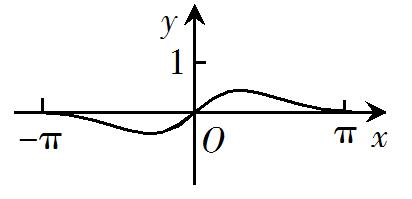
\includegraphics[width=.42\linewidth]{assets/asset-064-01.jpg}
\end{center}
\begin{choices}
  \item $\frac{5}{16}$
  \item $\frac{11}{32}$
  \item $\frac{21}{32}$
  \item $\frac{11}{16}$
\end{choices}
\begin{solution}
\textbf{答案：}$A$

\textbf{分析：}本题主要考查利用两个计数原理与排列组合计算古典概型问题，渗透了传统文化、数学计算等数学素养，“重卦”中每一爻有两种情况，基本事件计算是住店问题，该重卦恰有 $3$ 个阳爻是相同元素的排列问题，利用直接法即可计算．

\textbf{详解：}由题知，每一爻有 $2$ 种情况，一重卦的 $6$ 爻有 $2^6$ 情况，其中 $6$ 爻中恰有 $3$ 个阳爻情况有 $C_6^3$，所以该重卦恰有 $3$ 个阳爻的概率为 $\frac{C_6^3}{2^6} = \frac{5}{16}$，故选 $A$．
\end{solution}
\end{question}

\begin{question}[points=5]
\textbf{来源：}2019 年 全国I卷-理科，第 8 题\par
如图是求 $\frac{1}{2 + \frac{1}{2 + \frac{1}{2}}}$ 的程序框图，图中空白框中应填入

\begin{center}
  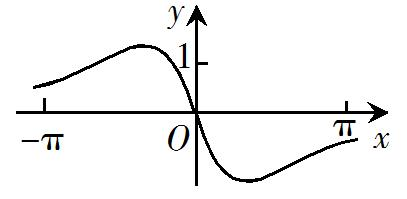
\includegraphics[width=.42\linewidth]{assets/asset-065-01.jpg}
\end{center}
\begin{choices}
  \item $A = \frac{1}{2 + A}$
  \item $A = 2 + \frac{1}{A}$
  \item $A = \frac{1}{1 + 2A}$
  \item $A = 1 + \frac{1}{2A}$
\end{choices}
\begin{solution}
\textbf{答案：}$A$

\textbf{分析：}本题主要考查算法中的程序框图，渗透阅读、分析与解决问题等素养，认真分析式子结构特征与程序框图结构，即可找出作出选择．

\textbf{详解：}执行第 $1$ 次，$A = \frac{1}{2}$, $k = 1 \le 2$ 是，因为第一次应该计算 $\frac{1}{2 + \frac{1}{2}} = \frac{1}{2 + A}$，$k = k + 1 = 2$，循环，执行第 $2$ 次，$k = 2 \le 2$，是，因为第二次应该计算 $\frac{1}{2 + \frac{1}{2 + \frac{1}{2}}} = \frac{1}{2 + A}$，$k = k + 1 = 3$，循环，执行第 $3$ 次，$k = 2 \le 2$，否，输出，故循环体为 $A = \frac{1}{2 + A}$，故选 $A$．
\end{solution}
\end{question}

\begin{question}[points=5]
\textbf{来源：}2019 年 全国I卷-理科，第 15 题\par
甲、乙两队进行篮球决赛，采取七场四胜制（当一队赢得四场胜利时，该队获胜，决赛结束）．根据前期比赛成绩，甲队的主客场安排依次为“主主客客主客主”．设甲队主场取胜的概率为 $0.6$，客场取胜的概率为 $0.5$，且各场比赛结果相互独立，则甲队以 $4 \colon 1$ 获胜的概率是．
\fillin[{$0.216$}]
\begin{solution}
\textbf{答案：}$0.216$

\textbf{分析：}本题应注意分情况讨论，即前五场甲队获胜的两种情况，应用独立事件的概率的计算公式求解．题目有一定的难度，注重了基础知识、基本计算能力及分类讨论思想的考查．

\textbf{详解：}前五场中有一场客场输时，甲队以 $4 \colon 1$ 获胜的概率是 $0.6^3 \times 0.5 \times 0.5 \times 2 = 0.108$, 前五场中有一场主场输时，甲队以 $4 \colon 1$ 获胜的概率是 $0.4 \times 0.6^2 \times 0.5^2 \times 3 = 0.108$, 综上所述，甲队以 $4 \colon 1$ 获胜的概率是 $0.108 + 0.108 = 0.216$．
\end{solution}
\end{question}

\begin{question}[points=12]
\textbf{来源：}2019 年 全国I卷-理科，第 21 题\par
为了治疗某种疾病，研制了甲、乙两种新药，希望知道哪种新药更有效，为此进行动物试验．试验方案如下：每一轮选取两只白鼠对药效进行对比试验．对于两只白鼠，随机选一只施以甲药，另一只施以乙药．一轮的治疗结果得出后，再安排下一轮试验．当其中一种药治愈的白鼠比另一种药治愈的白鼠多 $4$ 只时，就停止试验，并认为治愈只数多的药更有效．为了方便描述问题，约定：对于每轮试验，若施以甲药的白鼠治愈且施以乙药的白鼠未治愈则甲药得 $1$ 分，乙药得 $-1$ 分；若施以乙药的白鼠治愈且施以甲药的白鼠未治愈则乙药得 $1$ 分，甲药得 $-1$ 分；若都治愈或都未治愈则两种药均得 $0$ 分．甲、乙两种药的治愈率分别记为 $\alpha$ 和 $\beta$，一轮试验中甲药的得分记为 $X$．

(1) 求 $X$ 的分布列；

(2) 若甲药、乙药在试验开始时都赋予 $4$ 分，$p_i$ $(i = 0, 1, \cdots, 8)$ 表示“甲药的累计得分为 $i$ 时，最终认为甲药比乙药更有效”的概率，则 $p_0 = 0$, $p_8 = 1$, $p_i = a p_{i-1} + b p_i + c p_{i+1}$ $(i = 1, 2, \cdots, 7)$，其中 $a = P(X = -1)$, $b = P(X = 0)$, $c = P(X = 1)$. 假设 $\alpha = 0.5$, $\beta = 0.8$.

(i) 证明：$\{p_{i+1} - p_i\}$ $(i = 0, 1, 2, \cdots, 7)$ 为等比数列；

(ii) 求 $p_4$，并根据 $p_4$ 的值解释这种试验方案的合理性．
\begin{solution}
\textbf{答案：}(1) 见解析; (2)(i) 见解析; (ii) $p_4 = \frac{1}{257}$

\textbf{分析：}(1) 首先确定 $X$ 所有可能的取值，再来计算出每个取值对应的概率，从而可得分布列；(2)(i) 求解出 $a$, $b$, $c$ 的取值，可得 $p_i = 0.4p_{i-1} + 0.5p_i + 0.1p_{i+1}$ $(i = 1,2,\cdots,7)$，从而整理出符合等比数列定义的形式，问题得证；(ii) 列出证得的等比数列的通项公式，采用累加的方式，结合 $p_8$ 和 $p_0$ 的值可求得 $p_1$；再次利用累加法可求出 $p_4$．

\textbf{详解：}(1) 由题意可知 $X$ 所有可能的取值为：$-1$, $0$, $1$．$P(X = -1) = (1 - \alpha)\beta$; $P(X = 0) = \alpha\beta + (1 - \alpha)(1 - \beta)$; $P(X = 1) = \alpha(1 - \beta)$．则 $X$ 的分布列如下：
\begin{center}
\begin{tabular}{c|c|c|c}
$X$ & $-1$ & $0$ & $1$ \\ \hline
$P$ & $(1-\alpha)\beta$ & $\alpha\beta + (1-\alpha)(1-\beta)$ & $\alpha(1-\beta)$
\end{tabular}
\end{center}
(2) $\because \alpha = 0.5$, $\beta = 0.8$, $\therefore a = 0.5 \times 0.8 = 0.4$, $b = 0.5 \times 0.8 + 0.5 \times 0.2 = 0.5$, $c = 0.5 \times 0.2 = 0.1$．
(i) $\because p_i = a p_{i-1} + b p_i + c p_{i+1}$ $(i = 1,2,\cdots,7)$，即 $p_i = 0.4p_{i-1} + 0.5p_i + 0.1p_{i+1}$, 整理可得：$5p_i = 4p_{i-1} + p_{i+1}$, $\therefore p_{i+1} - p_i = 4(p_i - p_{i-1})$ $(i = 1,2,\cdots,7)$．又 $p_1 - p_0 = p_1 \neq 0$, $\therefore \{p_{i+1} - p_i\}$ $(i = 0,1,2,\cdots,7)$ 为公比为 $4$，首项为 $p_1$ 的等比数列．
(ii) 由 (i) 可得 $p_8 = p_8 - p_7 + p_7 - p_6 + \cdots + p_1 - p_0 + p_0 = (p_8 - p_7) + (p_7 - p_6) + \cdots + (p_1 - p_0) = \frac{4^8 - 1}{3}p_1$．由于 $p_8 = 1$, 故 $p_1 = \frac{3}{4^8 - 1}$, 所以 $p_4 = (p_4 - p_3) + (p_3 - p_2) + (p_2 - p_1) + (p_1 - p_0) = \frac{4^4 - 1}{3}p_1 = \frac{1}{257}$．$p_4$ 表示最终认为甲药更有效的概率，由计算结果可以看出，在甲药治愈率为 $0.5$，乙药治愈率为 $0.8$ 时，认为甲药更有效的概率为 $p_4 = \frac{1}{257} \approx 0.0039$，此时得出错误结论的概率非常小，说明这种试验方案合理．
\end{solution}
\end{question}

\begin{question}[points=5]
\textbf{来源：}2019 年 全国I卷-文科，第 6 题\par
某学校为了解 1000 名新生的身体素质，将这些学生编号为 1，2，…，1000，从这些新生中用系统抽样方法等距抽取 100 名学生进行体质测验．若 46 号学生被抽到，则下面 4 名学生中被抽到的是
\begin{choices}
  \item 8 号学生
  \item 200 号学生
  \item 616 号学生
  \item 815 号学生
\end{choices}
\begin{solution}
\textbf{答案：}C

\textbf{分析：}等差数列的性质．渗透了数据分析素养．使用统计思想，逐个选项判断得出答案。

\textbf{详解：}由已知将 1000 名学生分成 100 个组，每组 10 名学生，用系统抽样，46 号学生被抽到，所以第一组抽到 6 号，且每组抽到的学生号构成等差数列 $\{a_n\}$，公差 $d=10$，所以 $a_n = 6+10n$ ($n \in \mathbb{N}^*$)，若 $8=6+10n$，则 $n=\frac{1}{5}$，不合题意；若 $200=6+10n$，则 $n=19.4$，不合题意；若 $616=6+10n$，则 $n=60$，符合题意；若 $815=6+10n$，则 $n=80.9$，不合题意．故选 C。
\end{solution}
\end{question}

\begin{question}[points=5]
\textbf{来源：}2019 年 全国I卷-文科，第 9 题\par
如图是求 $2+\frac{1}{2+\frac{1}{2}}$ 的程序框图，图中空白框中应填入

\begin{center}
  
\includegraphics[width=.42\linewidth]{assets/asset-069-01.jpg}
\end{center}
\begin{choices}
  \item $A=\frac{1}{2+A}$
  \item $A=2+\frac{1}{A}$
  \item $A=\frac{1}{1+2A}$
  \item $A=1+\frac{1}{2A}$
\end{choices}
\begin{solution}
\textbf{答案：}A

\textbf{分析：}本题主要考查算法中的程序框图，认真分析式子结构特征与程序框图结构，即可找出作出选择。

\textbf{详解：}执行第 1 次，$A=\frac{1}{2}$，$k=1 \le 2$ 是，因为第一次应该计算 $\frac{1}{2+\frac{1}{2}} = \frac{1}{2+A}$，$k=k+1=2$，循环，执行第 2 次，$k=2 \le 2$，是，因为第二次应该计算 $2+\frac{1}{2+\frac{1}{2}} = \frac{1}{2+A}$，$k=k+1=3$，循环，执行第 3 次，$k=2 \le 2$，否，输出，故循环体为 $A=\frac{1}{2+A}$，故选 A。
\end{solution}
\end{question}

\begin{question}[points=12]
\textbf{来源：}2019 年 全国I卷-文科，第 17 题\par
某商场为提高服务质量，随机调查了 50 名男顾客和 50 名女顾客，每位顾客对该商场的服务给出满意或不满意的评价，得到下面列联表：



| | 满意 | 不满意 |

|-------|------|--------|

| 男顾客 | 40 | 10 |

| 女顾客 | 30 | 20 |



（1）分别估计男、女顾客对该商场服务满意的概率；

（2）能否有 95% 的把握认为男、女顾客对该商场服务的评价有差异？



附：$K^2 = \frac{n(ad-bc)^2}{(a+b)(c+d)(a+c)(b+d)}$，



| $P(K^2 \ge k)$ | 0.050 | 0.010 | 0.001 |

|----------------|-------|-------|-------|

| $k$ | 3.841 | 6.635 | 10.828 |
\begin{solution}
\textbf{答案：}（1）男顾客：$\frac{4}{5}$，女顾客：$\frac{3}{5}$；（2）能有 95% 的把握认为有差异。

\textbf{分析：}（1）从题中所给的 $2\times2$ 列联表中读出相关的数据，利用满意的人数除以总的人数，分别算出相应的频率，即估计得出的概率值；（2）利用公式求得观测值与临界值比较。

\textbf{详解：}（1）由题中表格可知，50 名男顾客对商场服务满意的有 40 人，所以男顾客对商场服务满意率估计为 $P_1 = \frac{40}{50} = \frac{4}{5}$；50 名女顾客对商场满意的有 30 人，所以女顾客对商场服务满意率估计为 $P_2 = \frac{30}{50} = \frac{3}{5}$。
（2）由列联表可知 $K^2 = \frac{100 \times (40 \times 20 - 30 \times 10)^2}{70 \times 30 \times 50 \times 50} = \frac{100}{21} \approx 4.762 > 3.841$，所以能有 95% 的把握认为男、女顾客对该商场服务的评价有差异。
\end{solution}
\end{question}

\section*{2020 年}

\begin{question}[points=5]
\textbf{来源：}2020 年 全国III卷-理科，第 3 题\par
在一组样本数据中，1,2,3,4 出现的频率分别为 $p_1,p_2,p_3,p_4$，且 $\sum\limits_{i=1}^4 p_i=1$，则下面四种情形中，对应样本的标准差最大的一组是
\begin{choices}
  \item $p_1=p_4=0.1,\ p_2=p_3=0.4$
  \item $p_1=p_4=0.4,\ p_2=p_3=0.1$
  \item $p_1=p_4=0.2,\ p_2=p_3=0.3$
  \item $p_1=p_4=0.3,\ p_2=p_3=0.2$
\end{choices}
\begin{solution}
\textbf{答案：}$B$

\textbf{分析：}计算出四个选项中对应数据的平均数和方差，由此可得出标准差最大的一组。

\textbf{详解：}对于 $A$ 选项，平均数为 $\overline{x}_A=(1+4)\times 0.1+(2+3)\times 0.4=2.5$，方差为 $s_A^2=(1-2.5)^2\times0.1+(2-2.5)^2\times0.4+(3-2.5)^2\times0.4+(4-2.5)^2\times0.1=0.65$。
对于 $B$ 选项，平均数为 $\overline{x}_B=(1+4)\times0.4+(2+3)\times0.1=2.5$，方差为 $s_B^2=(1-2.5)^2\times0.4+(2-2.5)^2\times0.1+(3-2.5)^2\times0.1+(4-2.5)^2\times0.4=1.85$。
对于 $C$ 选项，平均数为 $\overline{x}_C=(1+4)\times0.2+(2+3)\times0.3=2.5$，方差为 $s_C^2=(1-2.5)^2\times0.2+(2-2.5)^2\times0.3+(3-2.5)^2\times0.3+(4-2.5)^2\times0.2=1.05$。
对于 $D$ 选项，平均数为 $\overline{x}_D=(1+4)\times0.3+(2+3)\times0.2=2.5$，方差为 $s_D^2=(1-2.5)^2\times0.3+(2-2.5)^2\times0.2+(3-2.5)^2\times0.2+(4-2.5)^2\times0.3=1.45$。
因此 $B$ 组标准差最大。故选 $B$。
\end{solution}
\end{question}

\begin{question}[points=12]
\textbf{来源：}2020 年 全国III卷-理科，第 18 题\par
某学生兴趣小组随机调查了某市100天中每天的空气质量等级和当天到某公园锻炼的人次，整理数据得到下表（单位：天）：

\begin{table}[h]

\centering

\begin{tabular}{|c|c|c|c|}

\hline

\multirow{2}*{空气质量等级} & \multicolumn{3}{|c|}{锻炼人次} \\ \cline{2-4}

 & $[0,200]$ & $(200,400]$ & $(400,600]$ \\ \hline

1（优） & 2 & 16 & 25 \\ \hline

2（良） & 5 & 10 & 12 \\ \hline

3（轻度污染） & 6 & 7 & 8 \\ \hline

4（中度污染） & 7 & 2 & 0 \\ \hline

\end{tabular}

\end{table}

(1) 分别估计该市一天的空气质量等级为1,2,3,4的概率；

(2) 求一天中到该公园锻炼的平均人次的估计值（同一组中的数据用该组区间的中点值为代表）；

(3) 若某天的空气质量等级为1或2，则称这天“空气质量好”；若某天的空气质量等级为3或4，则称这天“空气质量不好”。根据所给数据，完成下面的 $2\times2$ 列联表，并根据列联表，判断是否有 $95\%$ 的把握认为一天中到该公园锻炼的人次与该市当天的空气质量有关？

\begin{center}

\begin{tabular}{|c|c|c|}

\hline

 & 人次 $\le400$ & 人次 $>400$ \\ \hline

空气质量好 & & \\ \hline

空气质量不好 & & \\ \hline

\end{tabular}

\end{center}

附：$K^2=\dfrac{n(ad-bc)^2}{(a+b)(c+d)(a+c)(b+d)}$，

\begin{center}

\begin{tabular}{c|ccc}

$P(K^2\ge k)$ & 0.050 & 0.010 & 0.001 \\ \hline

$k$ & 3.841 & 6.635 & 10.828 \\

\end{tabular}

\end{center}
\begin{solution}
\textbf{答案：}见解析

\textbf{分析：}(1) 根据频数分布表计算频率；(2) 利用每组中点值计算平均数；(3) 完善列联表，计算 $K^2$ 并与临界值比较。

\textbf{详解：}(1) 等级1的概率 $\dfrac{2+16+25}{100}=0.43$，等级2的概率 $\dfrac{5+10+12}{100}=0.27$，等级3的概率 $\dfrac{6+7+8}{100}=0.21$，等级4的概率 $\dfrac{7+2+0}{100}=0.09$。
(2) 平均人次 $\dfrac{100\times20+300\times35+500\times45}{100}=350$。
(3) $2\times2$ 列联表如下：
\begin{center}
\begin{tabular}{|c|c|c|}
\hline
 & 人次 $\le400$ & 人次 $>400$ \\ \hline
空气质量好 & 33 & 37 \\ \hline
空气质量不好 & 22 & 8 \\ \hline
\end{tabular}
\end{center}
$K^2=\dfrac{100\times(33\times8-37\times22)^2}{55\times45\times70\times30}\approx5.820>3.841$，所以有 $95\%$ 的把握认为有关。
\end{solution}
\end{question}

\begin{question}[points=5]
\textbf{来源：}2020 年 全国III卷-文科，第 3 题\par
设一组样本数据 $x_1,x_2,\dots,x_n$ 的方差为 $0.01$，则数据 $10x_1,10x_2,\dots,10x_n$ 的方差为
\begin{choices}
  \item $0.01$
  \item $0.1$
  \item $1$
  \item $10$
\end{choices}
\begin{solution}
\textbf{答案：}C

\textbf{分析：}根据新数据与原数据关系确定方差关系，即得结果.

\textbf{详解：}因为数据 $ax_i+b\ (i=1,2,\dots,n)$ 的方差是数据 $x_i\ (i=1,2,\dots,n)$ 的方差的 $a^2$ 倍，所以所求数据方差为 $10^2\times0.01=1$. 故选：C.
\end{solution}
\end{question}

\begin{question}[points=12]
\textbf{来源：}2020 年 全国III卷-文科，第 18 题\par
某学生兴趣小组随机调查了某市100天中每天的空气质量等级和当天到某公园锻炼的人次，整理数据得到下表(单位：天)：



| 锻炼人次 | [0,200] | (200,400] | (400,600] |

|----------|---------|-----------|-----------|

| 1(优)    | 2       | 16        | 25        |

| 2(良)    | 5       | 10        | 12        |

| 3(轻度污染) | 6    | 7         | 8         |

| 4(中度污染) | 7    | 2         | 0         |



(1) 分别估计该市一天的空气质量等级为1,2,3,4的概率；

(2) 求一天中到该公园锻炼的平均人次的估计值(同一组中的数据用该组区间的中点值为代表)；

(3) 若某天的空气质量等级为1或2，则称这天“空气质量好”；若某天的空气质量等级为3或4，则称这天“空气质量不好”。根据所给数据，完成下面的 $2\times2$ 列联表，并根据列联表，判断是否有95%的把握认为一天中到该公园锻炼的人次与该市当天的空气质量有关？



附：$K^2=\frac{n(ad-bc)^2}{(a+b)(c+d)(a+c)(b+d)}$，$P(K^2\geq3.841)\approx0.050$.
\begin{solution}
\textbf{答案：}(1) 概率分别为 $0.43$, $0.27$, $0.21$, $0.09$ (2) $350$ (3) 有

\textbf{分析：}(1)根据频数分布表可计算出该市一天的空气质量等级分别为 $1,2,3,4$ 的概率；(2)利用每组的中点值乘以频数，相加后除以100可得结果；(3)根据表格中的数据完善 $2\times2$ 列联表，计算出 $K^2$ 的观测值，再结合临界值表可得结论.

\textbf{详解：}(1) 由频数分布表可知，该市一天的空气质量等级为1的概率为 $\frac{2+16+25}{100}=0.43$，等级为2的概率为 $\frac{5+10+12}{100}=0.27$，等级为3的概率为 $\frac{6+7+8}{100}=0.21$，等级为4的概率为 $\frac{7+2+0}{100}=0.09$.
(2) 一天中到该公园锻炼的人次的平均数为 $\frac{100\times20+300\times35+500\times45}{100}=350$.
(3) $2\times2$ 列联表如下：

|          | 人次$\leq400$ | 人次$>400$ |
|----------|-------------|-----------|
| 空气质量好 | 33          | 37        |
| 空气质量不好 | 22          | 8         |

$K^2=\frac{100\times(33\times8-37\times22)^2}{55\times45\times70\times30}\approx5.820>3.841$，因此，有95%的把握认为一天中到该公园锻炼的人次与该市当天的空气质量有关.
\end{solution}
\end{question}

\begin{question}[points=5]
\textbf{来源：}2020 年 全国II卷-理科，第 3 题\par
在新冠肺炎疫情防控期间，某超市开通网上销售业务，每天能完成1200份订单的配货，由于订单量大幅增加，导致订单积压.为解决困难，许多志愿者踊跃报名参加配货工作.已知该超市某日积压500份订单未配货，预计第二天的新订单超过1600份的概率为0.05，志愿者每人每天能完成50份订单的配货，为使第二天完成积压订单及当日订单的配货的概率不小于0.95，则至少需要志愿者（ ）
\begin{choices}
  \item 10名
  \item 18名
  \item 24名
  \item 32名
\end{choices}
\begin{solution}
\textbf{答案：}18名

\textbf{分析：}算出第二天订单数，除以志愿者每天能完成的订单配货数即可.

\textbf{详解：}由题意，第二天新增订单数为 $500+1600-1200=900$，故需要志愿者 $\dfrac{900}{50}=18$ 名.
\end{solution}
\end{question}

\begin{question}[points=12]
\textbf{来源：}2020 年 全国II卷-理科，第 18 题\par
某沙漠地区经过治理，生态系统得到很大改善，野生动物数量有所增加.为调查该地区某种野生动物的数量，将其分成面积相近的200个地块，从这些地块中用简单随机抽样的方法抽取20个作为样区，调查得到样本数据$(x_i,y_i)(i=1,2,\ldots,20)$，其中$x_i$和$y_i$分别表示第$i$个样区的植物覆盖面积(单位：公顷)和这种野生动物的数量，并计算得$\sum\limits_{i=1}^{20}x_i=60$，$\sum\limits_{i=1}^{20}y_i=1200$，$\sum\limits_{i=1}^{20}(x_i-\overline{x})^2=80$，$\sum\limits_{i=1}^{20}(y_i-\overline{y})^2=9000$，$\sum\limits_{i=1}^{20}(x_i-\overline{x})(y_i-\overline{y})=800$.

（1）求该地区这种野生动物数量的估计值（这种野生动物数量的估计值等于样区这种野生动物数量的平均数乘以地块数）；

（2）求样本$(x_i,y_i)(i=1,2,\ldots,20)$的相关系数（精确到0.01）；

（3）根据现有统计资料，各地块间植物覆盖面积差异很大.为提高样本的代表性以获得该地区这种野生动物数量更准确的估计，请给出一种你认为更合理的抽样方法，并说明理由.

附：相关系数$r=\dfrac{\sum\limits_{i=1}^{n}(x_i-\overline{x})(y_i-\overline{y})}{\sqrt{\sum\limits_{i=1}^{n}(x_i-\overline{x})^2\sum\limits_{i=1}^{n}(y_i-\overline{y})^2}}$，$\sqrt2=1.414$.
\begin{solution}
\textbf{答案：}（1）12000；（2）0.94；（3）分层抽样，理由见解析.

\textbf{分析：}（1）利用野生动物数量的估计值等于样区野生动物平均数乘以地块数，代入数据即可；（2）利用公式$r=\dfrac{\sum(x_i-\overline{x})(y_i-\overline{y})}{\sqrt{\sum(x_i-\overline{x})^2\sum(y_i-\overline{y})^2}}$计算即可；（3）各地块间植物覆盖面积差异较大，为提高样本数据的代表性，应采用分层抽样.

\textbf{详解：}（1）样区野生动物平均数为$\dfrac1{20}\sum_{i=1}^{20}y_i=\dfrac{1}{20}\times1200=60$，地块数为200，该地区这种野生动物数量的估计值为$200\times60=12000$.
（2）样本$(x_i,y_i)$的相关系数为$r=\dfrac{\sum_{i=1}^{20}(x_i-\overline{x})(y_i-\overline{y})}{\sqrt{\sum_{i=1}^{20}(x_i-\overline{x})^2\sum_{i=1}^{20}(y_i-\overline{y})^2}}=\dfrac{800}{\sqrt{80\times9000}}=\dfrac{800}{\sqrt{720000}}=\dfrac{800}{600\sqrt2}=\dfrac{4}{3\sqrt2}=\dfrac{2\sqrt2}{3}\approx0.94$.
（3）由于各地块间植物覆盖面积差异较大，为提高样本的代表性，应采用分层抽样.先将植物覆盖面积按优中差分成三层，在各层内按比例抽取样本，在每层内用简单随机抽样法抽取样本即可.
\end{solution}
\end{question}

\begin{question}[points=5]
\textbf{来源：}2020 年 全国II卷-文科，第 4 题\par
在新冠肺炎疫情防控期间，某超市开通网上销售业务，每天能完成1200份订单的配货，由于订单量大幅增加，导致订单积压。为解决困难，许多志愿者踊跃报名参加配货工作。已知该超市某日积压500份订单未配货，预计第二天的新订单超过1600份的概率为0.05，志愿者每人每天能完成50份订单的配货，为使第二天完成积压订单及当日订单的配货的概率不小于0.95，则至少需要志愿者（ ）
\begin{choices}
  \item $10$名
  \item $18$名
  \item $24$名
  \item $32$名
\end{choices}
\begin{solution}
\textbf{答案：}B

\textbf{分析：}算出第二天订单数，除以志愿者每天能完成的订单配货数即可。

\textbf{详解：}由题意，第二天新增订单数为 $500+1600-1200=900$，故需要志愿者 $\frac{900}{50}=18$ 名。
故选：B。
\end{solution}
\end{question}

\begin{question}[points=12]
\textbf{来源：}2020 年 全国II卷-文科，第 18 题\par
某沙漠地区经过治理，生态系统得到很大改善，野生动物数量有所增加。为调查该地区某种野生动物的数量，将其分成面积相近的200个地块，从这些地块中用简单随机抽样的方法抽取20个作为样区，调查得到样本数据 $(x_i,y_i)(i=1,2,\ldots,20)$，其中 $x_i$ 和 $y_i$ 分别表示第 $i$ 个样区的植物覆盖面积（单位：公顷）和这种野生动物的数量，并计算得

$\sum_{i=1}^{20}x_i=60$，$\sum_{i=1}^{20}y_i=1200$，

$\sum_{i=1}^{20}(x_i-\bar{x})^2=80$，$\sum_{i=1}^{20}(y_i-\bar{y})^2=9000$，$\sum_{i=1}^{20}(x_i-\bar{x})(y_i-\bar{y})=800$。

（1）求该地区这种野生动物数量的估计值（这种野生动物数量的估计值等于样区这种野生动物数量的平均数乘以地块数）；

（2）求样本 $(x_i,y_i)(i=1,2,\ldots,20)$ 的相关系数（精确到0.01）；

（3）根据现有统计资料，各地块间植物覆盖面积差异很大。为提高样本的代表性以获得该地区这种野生动物数量更准确的估计，请给出一种你认为更合理的抽样方法，并说明理由。

附：相关系数 $r=\frac{\sum_{i=1}^{n}(x_i-\bar{x})(y_i-\bar{y})}{\sqrt{\sum_{i=1}^{n}(x_i-\bar{x})^2\sum_{i=1}^{n}(y_i-\bar{y})^2}}$，$\sqrt{2}=1.414$。
\begin{solution}
\textbf{答案：}（1）12000；（2）0.94；（3）详见解析。

\textbf{分析：}（1）利用野生动物数量的估计值等于样区野生动物平均数乘以地块数，代入数据即可；
（2）利用公式 $r=\frac{\sum_{i=1}^{20}(x_i-\bar{x})(y_i-\bar{y})}{\sqrt{\sum_{i=1}^{20}(x_i-\bar{x})^2\sum_{i=1}^{20}(y_i-\bar{y})^2}}$ 计算即可；
（3）各地块间植物覆盖面积差异较大，为提高样本数据的代表性，应采用分层抽样。

\textbf{详解：}（1）样区野生动物平均数为 $\frac{1}{20}\sum_{i=1}^{20}y_i = \frac{1}{20}\times1200=60$，
地块数为200，该地区这种野生动物的估计值为 $200\times60=12000$。
（2）样本 $(x_i,y_i)$ 的相关系数为
$r = \frac{\sum_{i=1}^{20}(x_i-\bar{x})(y_i-\bar{y})}{\sqrt{\sum_{i=1}^{20}(x_i-\bar{x})^2\sum_{i=1}^{20}(y_i-\bar{y})^2}} = \frac{800}{\sqrt{80\times9000}} = \frac{800}{\sqrt{720000}} = \frac{800}{600\sqrt{2}} = \frac{4}{3\sqrt{2}} = \frac{2\sqrt{2}}{3} \approx 0.94$。
（3）由于各地块间植物覆盖面积差异较大，为提高样本数据的代表性，应采用分层抽样。先将植物覆盖面积按优、中、差分成三层，在各层内按比例抽取样本，在每层内用简单随机抽样法抽取样本即可。
\end{solution}
\end{question}

\begin{question}[points=5]
\textbf{来源：}2020 年 全国I卷-理科，第 5 题\par
某校一个课外学习小组为研究某作物种子的发芽率$y$和温度$x$（单位：$^\circ$C）的关系，在20个不同的温度条件下进行种子发芽实验，由实验数据$(x_i,y_i)(i=1,2,\ldots,20)$得到下面的散点图。由此散点图，在$10^\circ$C至$40^\circ$C之间，下面四个回归方程类型中最适宜作为发芽率$y$和温度$x$的回归方程类型的是

\begin{center}
  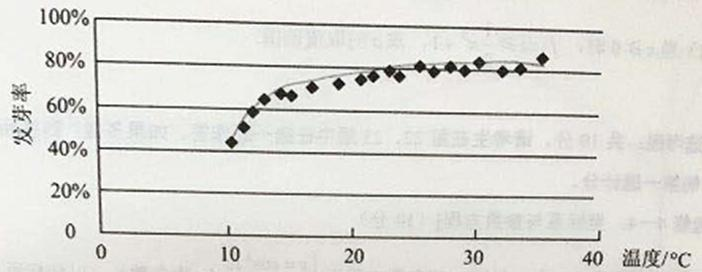
\includegraphics[width=.42\linewidth]{assets/asset-079-01.jpg}
\end{center}
\begin{choices}
  \item $y=a+bx$
  \item $y=a+bx^2$
  \item $y=a+be^x$
  \item $y=a+b\ln x$
\end{choices}
\begin{solution}
\textbf{答案：}D

\textbf{详解：}由散点图分布可知，散点图分布在一个对数函数的图象附近，因此最适合作为发芽率$y$和温度$x$的回归方程类型的是$y=a+b\ln x$。
\end{solution}
\end{question}

\begin{question}[points=12]
\textbf{来源：}2020 年 全国I卷-理科，第 19 题\par
甲、乙、丙三位同学进行羽毛球比赛，约定赛制如下：累计负两场者被淘汰；比赛前抽签决定首先比赛的两人，另一人轮空；每场比赛的胜者与轮空者进行下一场比赛，负者下一场轮空，直至有一人被淘汰；当一人被淘汰后，剩余的两人继续比赛，直至其中一人被淘汰，另一人最终获胜，比赛结束。经抽签，甲、乙首先比赛，丙轮空。设每场比赛双方获胜的概率都为$\frac{1}{2}$。

(1)求甲连胜四场的概率；

(2)求需要进行第五场比赛的概率；

(3)求丙最终获胜的概率。
\begin{solution}
\textbf{答案：}(1)$\frac{1}{16}$；(2)$\frac{3}{4}$；(3)$\frac{7}{16}$

\textbf{详解：}(1)甲连胜四场表示甲依次战胜乙、丙、乙、丙，概率$P=\left(\frac{1}{2}\right)^4=\frac{1}{16}$。
(2)四局内结束比赛的情况有：ABAB, ACAC, BCBC, BABA（其中A表示甲输，B表示乙输，C表示丙输），每种概率$\left(\frac{1}{2}\right)^4=\frac{1}{16}$，故四局内结束的概率$P'=4\times\frac{1}{16}=\frac{1}{4}$，因此需要进行第五场比赛的概率$1-P'=\frac{3}{4}$。
(3)丙最终获胜的情况（甲赢时）包括：BCBC, ABCBC, ACBCB, BABCC, BACBC, BCACB, BCABC, BCBAC，共8种，概率$P_{\text{甲}}=\left(\frac{1}{2}\right)^4+7\times\left(\frac{1}{2}\right)^5=\frac{1}{16}+\frac{7}{32}=\frac{9}{32}$。由对称性，乙赢的概率与甲相同，故丙赢的概率$P_{\text{丙}}=1-2\times\frac{9}{32}=\frac{7}{16}$。
\end{solution}
\end{question}

\begin{question}[points=5]
\textbf{来源：}2020 年 全国I卷-文科，第 4 题\par
设 $O$ 为正方形 $ABCD$ 的中心，在 $O, A, B, C, D$ 中任取 $3$ 点，则取到的 $3$ 点共线的概率为
\begin{choices}
  \item $\frac{1}{5}$
  \item $\frac{2}{5}$
  \item $\frac{1}{2}$
  \item $\frac{4}{5}$
\end{choices}
\begin{solution}
\textbf{答案：}$\frac{1}{5}$

\textbf{分析：}列出从 $5$ 个点选 $3$ 个点的所有情况，再列出 $3$ 点共线的情况，用古典概型的概率计算公式运算即可.

\textbf{详解：}从 $O,A,B,C,D$ 5个点中任取3个有10种不同取法，3点共线只有 $\{A,O,C\}$ 与 $\{B,O,D\}$ 共2种情况，由古典概型的概率计算公式知，取到3点共线的概率为 $\frac{2}{10} = \frac{1}{5}$.
\end{solution}
\end{question}

\begin{question}[points=5]
\textbf{来源：}2020 年 全国I卷-文科，第 5 题\par
某校一个课外学习小组为研究某作物种子的发芽率 $y$ 和温度 $x$ (单位：$^\circ$C)的关系，在 $20$ 个不同的温度条件下进行种子发芽实验，由实验数据 $(x_i, y_i)$ ($i=1,2,\cdots,20$) 得到下面的散点图： 由此散点图，在 $10^\circ$C 至 $40^\circ$C 之间，下面四个回归方程类型中最适宜作为发芽率 $y$ 和温度 $x$ 的回归方程类型的是

\begin{center}
  
\includegraphics[width=.42\linewidth]{assets/asset-082-01.jpg}
\end{center}
\begin{choices}
  \item $y = a + bx$
  \item $y = a + bx^2$
  \item $y = a + be^x$
  \item $y = a + b\ln x$
\end{choices}
\begin{solution}
\textbf{答案：}$y = a + b\ln x$

\textbf{分析：}根据散点图的分布可选择合适的函数模型.

\textbf{详解：}由散点图分布可知，散点图分布在一个对数函数的图象附近，因此，最适合作为发芽率 $y$ 和温度 $x$ 的回归方程类型的是 $y = a + b\ln x$.
\end{solution}
\end{question}

\begin{question}[points=12]
\textbf{来源：}2020 年 全国I卷-文科，第 17 题\par
某厂接受了一项加工业务，加工出来的产品(单位：件)按标准分为 $A, B, C, D$ 四个等级。加工业务约定：对于 $A$ 级品、$B$ 级品、$C$ 级品，厂家每件分别收取加工费 $90$ 元，$50$ 元，$20$ 元；对于 $D$ 级品，厂家每件要赔偿原料损失费 $50$ 元。该厂有甲、乙两个分厂可承接加工业务。甲分厂加工成本费为 $25$ 元/件，乙分厂加工成本费为 $20$ 元/件。厂家为决定由哪个分厂承接加工业务，在两个分厂各试加工了 $100$ 件这种产品，并统计了这些产品的等级，整理如下：



甲分厂产品等级的频数分布表



| 等级 | A | B | C | D |

|------|---|---|---|---|

| 频数 | 40 | 20 | 20 | 20 |



乙分厂产品等级的频数分布表



| 等级 | A | B | C | D |

|------|---|---|---|---|

| 频数 | 28 | 17 | 34 | 21 |



(1) 分别估计甲、乙两分厂加工出来的一件产品为 $A$ 级品的概率；



(2) 分别求甲、乙两分厂加工出来的 $100$ 件产品的平均利润，以平均利润为依据，厂家应选哪个分厂承接加工业务?
\begin{solution}
\textbf{答案：}(1) 甲分厂加工出来的 $A$ 级品的概率为 $0.4$, 乙分厂加工出来的 $A$ 级品的概率为 $0.28$; (2) 选甲分厂.

\textbf{分析：}(1) 根据两个频数分布表即可求出； (2) 根据题意分别求出甲乙两厂加工 $100$ 件产品的总利润，即可求出平均利润，由此作出选择.

\textbf{详解：}(1) 由表可知，甲厂加工出来的一件产品为 $A$ 级品的概率为 $\frac{40}{100}=0.4$, 乙厂加工出来的一件产品为 $A$ 级品的概率为 $\frac{28}{100}=0.28$.

(2) 甲分厂加工 $100$ 件产品的总利润为 $40\times(90-25)+20\times(50-25)+20\times(20-25)-20\times(50+25)=1500$ 元, 平均利润为 $15$ 元每件; 乙分厂加工 $100$ 件产品的总利润为 $28\times(90-20)+17\times(50-20)+34\times(20-20)-21\times(50+20)=1000$ 元, 平均利润为 $10$ 元每件. 故厂家选择甲分厂承接加工任务.
\end{solution}
\end{question}

\section*{2021 年}

\begin{question}[points=14]
\textbf{来源：}2021 年 北京卷，第 18 题\par
为加快新冠肺炎检测效率, 某检测机构采取“$k$ 合 $1$ 检测法”, 即将 $k$ 个人的拭子样本合并检测, 若为阴性, 则可以确定所有样本都是阴性的; 若为阳性, 则还需要对本组的每个人再做检测. 现有 $100$ 人, 已知其中 $2$ 人感染病毒.

(1) ①若采用“$10$ 合 $1$ 检测法”, 且两名患者在同一组, 求总检测次数;

②已知 $10$ 人分成一组, 分 $10$ 组, 两名感染患者在同一组的概率为 $\frac{1}{11}$, 定义随机变量 $X$ 为总检测次数, 求检测次数 $X$ 的分布列和数学期望 $E(X)$;

(2) 若采用“$5$ 合 $1$ 检测法”, 检测次数 $Y$ 的期望为 $E(Y)$, 试比较 $E(X)$ 和 $E(Y)$ 的大小(直接写出结果).
\begin{solution}
\textbf{答案：}(1) ① $20$ 次; ②分布列见解析, 期望为 $\frac{320}{11}$; (2) 见解析.

\textbf{分析：}(1) ①由题设条件还原情境, 即可得解; ②求出 $X$ 的取值情况及概率, 进而可得分布列和期望; (2) 求出 $E(Y)$, 分类比较.

\textbf{详解：}(1) ①对每组进行检测, 需要 $10$ 次; 再对结果为阳性的组每个人进行检测, 需要 $10$ 次; 所以总检测次数为 $20$ 次.
②由题意, $X$ 可以取 $20,30$, $P(X=20)=\frac{1}{11}$, $P(X=30)=1-\frac{1}{11}=\frac{10}{11}$, 分布列为:
| $X$ | $20$ | $30$ |
|-----|-----|-----|
| $P$ | $\frac{1}{11}$ | $\frac{10}{11}$ |
所以 $E(X)=20\times\frac{1}{11}+30\times\frac{10}{11}=\frac{320}{11}$.
(2) 由题意, $Y$ 可以取 $25,30$, 设两名感染者在同一组的概率为 $p$, $P(Y=25)=p$, $P(Y=30)=1-p$, 则 $E(Y)=25p+30(1-p)=30-5p$. 若 $p=\frac{2}{11}$, $E(X)=E(Y)$; 若 $p>\frac{2}{11}$, $E(X)>E(Y)$; 若 $p<\frac{2}{11}$, $E(X)<E(Y)$.
\end{solution}
\end{question}

\begin{question}[points=5]
\textbf{来源：}2021 年 全国甲卷-理科，第 2 题\par
为了解某地农村经济情况，对该地农户家庭年收入进行抽样调查，将农户家庭年收入的调查数据整理得到如下频率分布直方图：根据此频率分布直方图，下面结论中不正确的是（ ）

\begin{center}
  
\includegraphics[width=.42\linewidth]{assets/asset-085-01.jpg}
\end{center}
\begin{choices}
  \item 该地农户家庭年收入低于4.5万元的农户比率估计为6%
  \item 该地农户家庭年收入不低于10.5万元的农户比率估计为10%
  \item 估计该地农户家庭年收入的平均值不超过6.5万元
  \item 估计该地有一半以上的农户，其家庭年收入介于4.5万元至8.5万元之间
\end{choices}
\begin{solution}
\textbf{答案：}C

\textbf{分析：}根据直方图的意义直接计算相应范围内的频率，即可判定ABD，以各组的中间值作为代表乘以相应的频率，然后求和即得到样本的平均数的估计值，也就是总体平均值的估计值，计算后即可判定C．

\textbf{详解：}由频率分布直方图可得：$0.02+0.04=0.06=6\%$，故A正确；$0.04+0.02\times3=0.10=10\%$，故B正确；$0.10+0.14+0.20\times2=0.64=64\%>50\%$，故D正确；平均值估计为$3\times0.02+4\times0.04+5\times0.10+6\times0.14+7\times0.20+8\times0.20+9\times0.10+10\times0.10+11\times0.04+12\times0.02+13\times0.02+14\times0.02=7.68$万元，超过6.5万元，故C错误．
\end{solution}
\end{question}

\begin{question}[points=5]
\textbf{来源：}2021 年 全国甲卷-理科，第 10 题；次专题：计数原理\par
将4个1和2个0随机排成一行，则2个0不相邻的概率为（ ）
\begin{choices}
  \item $\frac{1}{3}$
  \item $\frac{2}{5}$
  \item $\frac{2}{3}$
  \item $\frac{4}{5}$
\end{choices}
\begin{solution}
\textbf{答案：}C

\textbf{分析：}采用插空法，4个1产生5个空，分2个0相邻和2个0不相邻进行求解．

\textbf{详解：}4个1和2个0随机排成一行，总情况数为 $C_6^2 = 15$（或 $\frac{6!}{4!2!} = 15$）．2个0不相邻的排法：先排4个1有1种，再将2个0插入5个空，有 $C_5^2 = 10$ 种，所以概率为 $\frac{10}{15} = \frac{2}{3}$．
\end{solution}
\end{question}

\begin{question}[points=12]
\textbf{来源：}2021 年 全国甲卷-理科，第 17 题\par
甲、乙两台机床生产同种产品，产品按质量分为一级品和二级品，为了比较两台机床产品的质量，分别用两台机床各生产了200件产品，产品的质量情况统计如下表：\begin{tabular}{|c|c|c|c|} \hline & 一级品 & 二级品 & 合计 \\ \hline 甲机床 & 150 & 50 & 200 \\ \hline 乙机床 & 120 & 80 & 200 \\ \hline 合计 & 270 & 130 & 400 \\ \hline \end{tabular}（1）甲机床、乙机床生产的产品中一级品的频率分别是多少？（2）能否有99%的把握认为甲机床的产品质量与乙机床的产品质量有差异？附：$K^2 = \frac{n(ad-bc)^2}{(a+b)(c+d)(a+c)(b+d)}$，$P(K^2 \ge k)$：0.050、0.010、0.001对应 $k$：3.841、6.635、10.828．
\begin{solution}
\textbf{答案：}（1）75%；60%；（2）能．

\textbf{分析：}本题考查频率统计和独立性检验，根据给出公式计算即可．

\textbf{详解：}（1）甲机床一级品频率为 $\frac{150}{200}=75\%$，乙机床一级品频率为 $\frac{120}{200}=60\%$．（2）$K^2 = \frac{400\times(150\times80-50\times120)^2}{270\times130\times200\times200} = \frac{400}{39} \approx 10.256 > 6.635$，所以有99%的把握认为甲机床的产品质量与乙机床有差异．
\end{solution}
\end{question}

\begin{question}[points=5]
\textbf{来源：}2021 年 全国甲卷-文科，第 2 题\par
为了解某地农村经济情况，对该地农户家庭年收入进行抽样调查，将农户家庭年收入的调查数据整理得到如下频率分布直方图：



根据此频率分布直方图，下面结论中不正确的是（ ）

\begin{center}
  
\includegraphics[width=.42\linewidth]{assets/asset-088-01.jpg}
\end{center}
\begin{choices}
  \item A. 该地农户家庭年收入低于4.5万元的农户比率估计为6%
  \item B. 该地农户家庭年收入不低于10.5万元的农户比率估计为10%
  \item C. 估计该地农户家庭年收入的平均值不超过6.5万元
  \item D. 估计该地有一半以上的农户，其家庭年收入介于4.5万元至8.5万元之间
\end{choices}
\begin{solution}
\textbf{答案：}C

\textbf{分析：}根据直方图的意义直接计算相应范围内的频率，即可判定ABD,以各组的中间值作为代表乘以相应的频率，然后求和即得到样本的平均数的估计值，也就是总体平均值的估计值，计算后即可判定C.

\textbf{详解：}因为频率直方图中的组距为1，所以各组的直方图的高度等于频率.样本频率直方图中的频率即可作为总体的相应比率的估计值.

该地农户家庭年收入低于4.5万元的农户的比率估计值为 $0.02+0.04=0.06=6\%$ ,故A正确；
该地农户家庭年收入不低于10.5万元的农户比率估计值为 $0.04+0.02\times3=0.10=10\%$ ,故B正确；
该地农户家庭年收入介于4.5万元至8.5万元之间的比例估计值为 $0.10+0.14+0.20\times2=0.64=64\%>50\%$ ,故D正确；
该地农户家庭年收入的平均值的估计值为 $3\times0.02+4\times0.04+5\times0.10+6\times0.14+7\times0.20+8\times0.20+9\times0.10+10\times0.10+11\times0.04+12\times0.02+13\times0.02+14\times0.02=7.68$ (万元)，超过6.5万元，故C错误.
综上，给出结论中不正确的是C.
\end{solution}
\end{question}

\begin{question}[points=5]
\textbf{来源：}2021 年 全国甲卷-文科，第 10 题；次专题：计数原理\par
将3个1和2个0随机排成一行，则2个0不相邻的概率为（ ）
\begin{choices}
  \item 0.3
  \item 0.5
  \item 0.6
  \item 0.8
\end{choices}
\begin{solution}
\textbf{答案：}C

\textbf{分析：}利用古典概型的概率公式可求概率.

\textbf{详解：}将3个1和2个0随机排成一行，共有10种排法：00111,01011,01101,01110,10011,10101,10110,11001,11010,11100. 其中2个0不相邻的排列有6种：01011,01101,01110,10101,10110,11010. 故概率为 $\frac{6}{10}=0.6$.
\end{solution}
\end{question}

\begin{question}[points=12]
\textbf{来源：}2021 年 全国甲卷-文科，第 17 题\par
甲、乙两台机床生产同种产品，产品按质量分为一级品和二级品，为了比较两台机床产品的质量，分别用两台机床各生产了200件产品，产品的质量情况统计如下表：



|        | 一级品 | 二级品 | 合计 |

|--------|--------|--------|------|

| 甲机床 | 150    | 50     | 200  |

| 乙机床 | 120    | 80     | 200  |

| 合计   | 270    | 130    | 400  |



（1）甲机床、乙机床生产的产品中一级品的频率分别是多少?



（2）能否有99%的把握认为甲机床的产品质量与乙机床的产品质量有差异?



附：$K^2 = \frac{n(ad-bc)^2}{(a+b)(c+d)(a+c)(b+d)}$



$P(K^2 \ge k)$  0.050  0.010  0.001



$k$          3.841  6.635  10.828
\begin{solution}
\textbf{答案：}（1）75%；60%；（2）能.

\textbf{分析：}根据给出公式计算即可.

\textbf{详解：}（1）甲机床生产的产品中的一级品的频率为 $\frac{150}{200}=75\%$, 乙机床生产的产品中的一级品的频率为 $\frac{120}{200}=60\%$.

（2）$K^2 = \frac{400 \times (150\times80 - 120\times50)^2}{270\times130\times200\times200} = \frac{400}{39} \approx 10.256 > 6.635$, 故能有99%的把握认为甲机床的产品与乙机床的产品质量有差异.
\end{solution}
\end{question}

\begin{question}[points=5]
\textbf{来源：}2021 年 全国乙卷-理科，第 8 题\par
在区间$(0,1)$与$(1,2)$中各随机取1个数，则两数之和大于$\frac74$的概率为（  ）

\begin{center}
  
\includegraphics[width=.42\linewidth]{assets/asset-091-01.jpg}
\end{center}
\begin{choices}
  \item $\frac79$
  \item $\frac{23}{32}$
  \item $\frac{9}{32}$
  \item $\frac29$
\end{choices}
\begin{solution}
\textbf{答案：}$\frac{23}{32}$

\textbf{详解：}由题意记$x\in(0,1)$，$y\in(1,2)$，即求$x+y>\frac74$的概率。绘图如下所示。故$P=\frac{S_{\text{阴}}}{S_{\text{正ABCD}}}=\frac{1\times1-\frac12\cdot AM\cdot AN}{1\times1}=1-\frac12\times\frac34\times\frac34=\frac{23}{32}$。故选B。
\end{solution}
\end{question}

\begin{question}[points=12]
\textbf{来源：}2021 年 全国乙卷-理科，第 17 题\par
某厂研制了一种生产高精产品的设备，为检验新设备生产产品的某项指标有无提高，用一台旧设备和一台新设备各生产了10件产品，得到各件产品该项指标数据如下：

旧设备：9.8, 10.3, 10.0, 10.2, 9.9, 9.8, 10.0, 10.1, 10.2, 9.7

新设备：10.1, 10.4, 10.1, 10.0, 10.1, 10.3, 10.6, 10.5, 10.4, 10.5

旧设备和新设备生产产品的该项指标的样本平均数分别记为$\bar{x}$和$\bar{y}$，样本方差分别记为$s_1^2$和$s_2^2$。

（1）求$\bar{x}$，$\bar{y}$，$s_1^2$，$s_2^2$；

（2）判断新设备生产产品的该项指标的均值较旧设备是否有显著提高（如果$\bar{y}-\bar{x}\geq 2\sqrt{\frac{s_1^2+s_2^2}{10}}$，则认为新设备生产产品的该项指标的均值较旧设备有显著提高，否则不认为有显著提高）。
\begin{solution}
\textbf{答案：}（1）$\bar{x}=10.0$，$\bar{y}=10.3$，$s_1^2=0.036$，$s_2^2=0.04$；（2）不认为有显著提高。

\textbf{详解：}（1）$\bar{x}=\frac1{10}(9.8+10.3+10.0+10.2+9.9+9.8+10.0+10.1+10.2+9.7)=10.0$，$\bar{y}=\frac1{10}(10.1+10.4+10.1+10.0+10.1+10.3+10.6+10.5+10.4+10.5)=10.3$，$s_1^2=\frac1{10}[(9.7-10.0)^2+2\times(9.8-10.0)^2+(9.9-10.0)^2+2\times(10.0-10.0)^2+(10.1-10.0)^2+2\times(10.2-10.0)^2+(10.3-10.0)^2]=0.036$，$s_2^2=\frac1{10}[(10.0-10.3)^2+3\times(10.1-10.3)^2+(10.3-10.3)^2+2\times(10.4-10.3)^2+2\times(10.5-10.3)^2+(10.6-10.3)^2]=0.04$。
（2）由（1）中数据得$\bar{y}-\bar{x}=0.3$，$2\sqrt{\frac{s_1^2+s_2^2}{10}}=2\sqrt{\frac{0.036+0.04}{10}}\approx0.34$。显然$\bar{y}-\bar{x}<2\sqrt{\frac{s_1^2+s_2^2}{10}}$。所以不认为新设备生产产品的该项指标的均值较旧设备有显著提高。
\end{solution}
\end{question}

\begin{question}[points=5]
\textbf{来源：}2021 年 全国乙卷-文科，第 7 题\par
在区间 $(0,\frac{1}{2})$ 随机取1个数，则取到的数小于 $\frac{1}{3}$ 的概率为（ ）
\begin{choices}
  \item $\frac{3}{4}$
  \item $\frac{2}{3}$
  \item $\frac{1}{3}$
  \item $\frac{1}{6}$
\end{choices}
\begin{solution}
\textbf{答案：}B

\textbf{分析：}在区间 $(0,\frac{1}{2})$ 随机取1个数，可知总长度 $d = \frac{1}{2}$ ，取到的数小于 $\frac{1}{3}$ ，可知取到的长度范围 $d' = \frac{1}{3}$ ，根据几何概型公式 $p = \frac{d'}{d} = \frac{\frac{1}{3}}{\frac{1}{2}} = \frac{2}{3}$ .
\end{solution}
\end{question}

\begin{question}[points=12]
\textbf{来源：}2021 年 全国乙卷-文科，第 17 题\par
某厂研制了一种生产高精产品的设备，为检验新设备生产产品的某项指标有无提高，用一台旧设备和一台新设备各生产了10件产品，得到各件产品该项指标数据如下：



旧设备：9.8, 10.3, 10.0, 10.2, 9.9, 9.8, 10.0, 10.1, 10.2, 9.7



新设备：10.1, 10.4, 10.1, 10.0, 10.1, 10.3, 10.6, 10.5, 10.4, 10.5



旧设备和新设备生产产品的该项指标的样本平均数分别记为 $\bar{x}$ 和 $\bar{y}$ ，样本方差分别记为 $s_1^2$ 和 $s_2^2$ .



（1）求 $\bar{x}$ ， $\bar{y}$ ， $s_1^2$ ， $s_2^2$ ；



（2）判断新设备生产产品的该项指标的均值较旧设备是否有显著提高（如果 $\bar{y} - \bar{x} \ge 2\sqrt{\frac{s_1^2 + s_2^2}{10}}$ ，则认为新设备生产产品的该项指标的均值较旧设备有显著提高，否则不认为有显著提高）. 
\begin{solution}
\textbf{答案：}见解析

\textbf{详解：}（1）$\bar{x} = \frac{9.8+10.3+10.0+10.2+9.9+9.8+10.0+10.1+10.2+9.7}{10} = 10$ ；
$\bar{y} = \frac{10.1+10.4+10.1+10.0+10.1+10.3+10.6+10.5+10.4+10.5}{10} = 10.3$ .
$s_1^2 = \frac{1}{10}(0.04+0.09+0.04+0.01+0.04+0.01+0.04+0.09) = \frac{1}{10}\times0.36 = 0.036$ ；
$s_2^2 = \frac{1}{10}(0.04+0.01+0.04+0.09+0.04+0.09+0.04+0.01+0.04) = \frac{1}{10}\times0.4 = 0.04$ .
（2）$\bar{y} - \bar{x} = 10.3 - 10 = 0.3$ ，
$2\sqrt{\frac{s_1^2 + s_2^2}{10}} = 2\sqrt{\frac{0.036+0.04}{10}} = 2\sqrt{0.0076}$ .
因为 $0.3 = \sqrt{0.09} > 2\sqrt{0.0076} = \sqrt{0.0304}$ ，所以可判断新设备生产产品的该项指标的均值较旧设备有显著提高.
\end{solution}
\end{question}

\begin{question}[points=5]
\textbf{来源：}2021 年 上海卷，第 10 题\par
甲、乙两人在花博会的$A$、$B$、$C$、$D$不同展馆中各选2个去参观，则两人选择中恰有一个馆相同的概率为．
\fillin[{$\frac{2}{3}$}]
\begin{solution}
\textbf{答案：}$\frac{2}{3}$

\textbf{分析：}注意“阅读，理解”，等价为“两个”排列组合题；

\textbf{详解：}由题意$A$、$B$、$C$、$D$四个不同的场馆，每人可选择的参观方法有：$C_4^2$种，则甲、乙两个人每人选2个场馆的参观方法有：$C_4^2\cdot C_4^2$种；由此，甲、乙两人恰好参观同一个场馆的参观方法有：$C_4^1\cdot C_3^1\cdot C_2^1$种；所以，甲、乙两人恰好参观同一个场馆的概率为：$p=\frac{C_4^1\cdot C_3^1\cdot C_2^1}{C_4^2\cdot C_4^2}=\frac{24}{36}=\frac{2}{3}$
\end{solution}
\end{question}

\begin{question}[points=5]
\textbf{来源：}2021 年 天津卷，第 4 题\par
从某网络平台推荐的影视作品中抽取400部，统计其评分数据，将所得400个评分数据分为8组：$[66,70)$，$[70,74)$，$\ldots$，$[94,98]$，并整理得到如下的频率分布直方图，则评分在区间 $[82,86)$ 内的影视作品数量是（   ）

\begin{center}
  
\includegraphics[width=.42\linewidth]{assets/asset-096-01.jpg}
\end{center}
\begin{choices}
  \item 20
  \item 40
  \item 64
  \item 80
\end{choices}
\begin{solution}
\textbf{答案：}D

\textbf{分析：}利用频率分布直方图可计算出评分在区间 $[82,86)$ 内的影视作品数量.

\textbf{详解：}由频率分布直方图可知，评分在区间 $[82,86)$ 内的影视作品数量为 $400 \times 0.05 \times 4 = 80$. 故选：D.
\end{solution}
\end{question}

\begin{question}[points=5]
\textbf{来源：}2021 年 天津卷，第 14 题\par
甲、乙两人在每次猜谜活动中各猜一个谜语，若一方猜对且另一方猜错，则猜对的一方获胜，否则本次平局，已知每次活动中，甲、乙猜对的概率分别为 $\frac{5}{6}$ 和 $\frac{1}{5}$，且每次活动中甲、乙猜对与否互不影响，各次活动也互不影响，则一次活动中，甲获胜的概率为，3次活动中，甲至少获胜2次的概率为.
\fillin[{$\frac{2}{3}$；$\frac{20}{27}$}]
\begin{solution}
\textbf{答案：}$\frac{2}{3}$；$\frac{20}{27}$

\textbf{分析：}根据甲猜对乙没有才对可求出一次活动中，甲获胜的概率；在3次活动中，甲至少获胜2次分为甲获胜2次和3次都获胜求解.

\textbf{详解：}一次活动中，甲获胜的概率为 $\frac{5}{6} \times \left(1-\frac{1}{5}\right) = \frac{5}{6} \times \frac{4}{5} = \frac{2}{3}$；3次活动中，甲至少获胜2次的概率为 $C_3^2 \left(\frac{2}{3}\right)^2 \times \frac{1}{3} + \left(\frac{2}{3}\right)^3 = \frac{12}{27} + \frac{8}{27} = \frac{20}{27}$.
\end{solution}
\end{question}

\begin{question}[points=5]
\textbf{来源：}2021 年 新高考II卷，第 6 题\par
某物理量的测量结果服从正态分布$N(10,\sigma^2)$，下列结论中不正确的是（ ）
\begin{choices}
  \item A. $\sigma$越小，该物理量在一次测量中在$(9.9,10.1)$的概率越大
  \item B. $\sigma$越小，该物理量在一次测量中大于$10$的概率为$0.5$
  \item C. $\sigma$越小，该物理量在一次测量中小于$9.99$与大于$10.01$的概率相等
  \item D. $\sigma$越小，该物理量在一次测量中落在$(9.9,10.2)$与落在$(10,10.3)$的概率相等
\end{choices}
\begin{solution}
\textbf{答案：}D

\textbf{分析：}由正态分布密度曲线的特征逐项判断即可得解.

\textbf{详解：}对于A，$\sigma^2$为数据的方差，所以$\sigma$越小，数据在$\mu=10$附近越集中，所以测量结果落在$(9.9,10.1)$内的概率越大，故A正确；对于B，由正态分布密度曲线的对称性可知该物理量一次测量大于10的概率为0.5，故B正确；对于C，由正态分布密度曲线的对称性可知该物理量一次测量结果大于10.01的概率与小于9.99的概率相等，故C正确；对于D，因为该物理量一次测量结果落在$(9.9,10.0)$的概率与落在$(10.2,10.3)$的概率不同，所以一次测量结果落在$(9.9,10.2)$的概率与落在$(10,10.3)$的概率不同，故D错误.故选：D.
\end{solution}
\end{question}

\begin{question}[points=5]
\textbf{来源：}2021 年 新高考II卷，第 9 题\par
下列统计量中，能度量样本$x_1,x_2,\cdots,x_n$的离散程度的是（ ）
\begin{choices}
  \item A. 样本$x_1,x_2,\cdots,x_n$的标准差
  \item B. 样本$x_1,x_2,\cdots,x_n$的中位数
  \item C. 样本$x_1,x_2,\cdots,x_n$的极差
  \item D. 样本$x_1,x_2,\cdots,x_n$的平均数
\end{choices}
\begin{solution}
\textbf{答案：}AC

\textbf{分析：}考查所给的选项哪些是考查数据的离散程度，哪些是考查数据的集中趋势即可确定正确选项.

\textbf{详解：}由标准差的定义可知，标准差考查的是数据的离散程度；由中位数的定义可知，中位数考查的是数据的集中趋势；由极差的定义可知，极差考查的是数据的离散程度；由平均数的定义可知，平均数考查的是数据的集中趋势；故选：AC.
\end{solution}
\end{question}

\begin{question}[points=12]
\textbf{来源：}2021 年 新高考II卷，第 21 题\par
一种微生物群体可以经过自身繁殖不断生存下来，设一个这种微生物为第$0$代，经过一次繁殖后为第$1$代，再经过一次繁殖后为第$2$代……，该微生物每代繁殖的个数是相互独立的且有相同的分布列，设$X$表示$1$个微生物个体繁殖下一代的个数，$P(X=i)=p_i(i=0,1,2,3)$．

（1）已知$p_0=0.4,p_1=0.3,p_2=0.2,p_3=0.1$，求$E(X)$；

（2）设$p$表示该种微生物经过多代繁殖后临近灭绝的概率，$p$是关于$x$的方程：$p_0+p_1x+p_2x^2+p_3x^3=x$的一个最小正实根，求证：当$E(X)\leq1$时，$p=1$，当$E(X)>1$时，$p<1$；

（3）根据你的理解说明（2）问结论的实际含义．
\begin{solution}
\textbf{答案：}(1) $1$；(2) 证明见解析；(3) 见解析.

\textbf{分析：}(1)利用公式计算可得$E(X)$； (2)利用导数讨论函数的单调性，结合$f(1)=0$及极值点的范围可得$f(x)$的最小正零点； (3)利用期望的意义及根的范围可得相应的理解说明.

\textbf{详解：}(1) $E(X)=0\times0.4+1\times0.3+2\times0.2+3\times0.1=1$． (2)设$f(x)=p_3x^3+p_2x^2+(p_1-1)x+p_0$，因为$p_3+p_2+p_1+p_0=1$，故$f(x)=p_3x^3+p_2x^2-(p_2+p_0+p_3)x+p_0$，若$E(X)\leq1$，则$p_1+2p_2+3p_3\leq1$，故$p_2+2p_3\leq p_0$．$f'(x)=3p_3x^2+2p_2x-(p_2+p_0+p_3)$，因为$f'(0)=-(p_2+p_0+p_3)<0$，$f'(1)=p_2+2p_3-p_0\leq0$，故$f'(x)$有两个不同零点$x_1,x_2$，且$x_1<0<1\leq x_2$，且$x\in(-\infty,x_1)\cup(x_2,+\infty)$时，$f'(x)>0$；$x\in(x_1,x_2)$时，$f'(x)<0$；故$f(x)$在$(-\infty,x_1)$，$(x_2,+\infty)$上为增函数，在$(x_1,x_2)$上为减函数，若$x_2=1$，因为$f(x)$在$(x_2,+\infty)$为增函数且$f(1)=0$，而当$x\in(0,x_2)$时，因为$f(x)$在$(x_1,x_2)$上为减函数，故$f(x)>f(x_2)=f(1)=0$，故$1$为$p_0+p_1x+p_2x^2+p_3x^3=x$的一个最小正实根，若$x_2>1$，因为$f(1)=0$且在$(0,x_2)$上为减函数，故$1$为$p_0+p_1x+p_2x^2+p_3x^3=x$的一个最小正实根，综上，若$E(X)\leq1$，则$p=1$．若$E(X)>1$，则$p_1+2p_2+3p_3>1$，故$p_2+2p_3>p_0$．此时$f'(0)=-(p_2+p_0+p_3)<0$，$f'(1)=p_2+2p_3-p_0>0$，故$f'(x)$有两个不同零点$x_3,x_4$，且$x_3<0<x_4<1$，且$x\in(-\infty,x_3)\cup(x_4,+\infty)$时，$f'(x)>0$；$x\in(x_3,x_4)$时，$f'(x)<0$；故$f(x)$在$(-\infty,x_3)$，$(x_4,+\infty)$上为增函数，在$(x_3,x_4)$上为减函数，而$f(1)=0$，故$f(x_4)<0$，又$f(0)=p_0>0$，故$f(x)$在$(0,x_4)$存在一个零点$p$，且$p<1$．所以$p$为$p_0+p_1x+p_2x^2+p_3x^3=x$的一个最小正实根，此时$p<1$，故当$E(X)>1$时，$p<1$． (3)意义：每一个该种微生物繁殖后代的平均数不超过$1$，则若干代必然灭绝，若繁殖后代的平均数超过$1$，则若干代后被灭绝的概率小于$1$.
\end{solution}
\end{question}

\begin{question}[points=5]
\textbf{来源：}2021 年 新高考I卷，第 8 题\par
有6个相同的球, 分别标有数字1,2,3,4,5,6, 从中有放回的随机取两次, 每次取1个球. 甲表示事件“第一次取出的球的数字是1”, 乙表示事件“第二次取出的球的数字是2”, 丙表示事件“两次取出的球的数字之和是8”, 丁表示事件“两次取出的球的数字之和是7”, 则 ( )
\begin{choices}
  \item 甲与丙相互独立
  \item 甲与丁相互独立
  \item 乙与丙相互独立
  \item 丙与丁相互独立
\end{choices}
\begin{solution}
\textbf{答案：}甲与丁相互独立

\textbf{分析：}根据独立事件概率关系逐一判断.

\textbf{详解：}$P(\text{甲}) = \frac{1}{6}$, $P(\text{乙}) = \frac{1}{6}$, $P(\text{丙}) = \frac{5}{36}$, $P(\text{丁}) = \frac{6}{36} = \frac{1}{6}$. $P(\text{甲丙}) = 0 \neq P(\text{甲})P(\text{丙})$, $P(\text{甲丁}) = \frac{1}{36} = P(\text{甲})P(\text{丁})$, $P(\text{乙丙}) = \frac{1}{36} \neq P(\text{乙})P(\text{丙})$, $P(\text{丙丁}) = 0 \neq P(\text{丁})P(\text{丙})$, 故选B.
\end{solution}
\end{question}

\begin{question}[points=5]
\textbf{来源：}2021 年 新高考I卷，第 9 题\par
有一组样本数据 $x_1, x_2, \ldots, x_n$, 由这组数据得到新样本数据 $y_1, y_2, \ldots, y_n$, 其中 $y_i = x_i + c$ ($i = 1,2,\ldots,n$), $c$ 为非零常数, 则 ( )
\begin{choices}
  \item 两组样本数据的样本平均数相同
  \item 两组样本数据的样本中位数相同
  \item 两组样本数据的样本标准差相同
  \item 两组样本数据的样本极差相同
\end{choices}
\begin{solution}
\textbf{答案：}C, D

\textbf{分析：}A、C利用两组数据的线性关系有 $E(y) = E(x) + c$, $D(y) = D(x)$, 即可判断; 根据中位数、极差的定义, 结合已知线性关系可判断B、D.

\textbf{详解：}A: $E(y) = E(x+c) = E(x) + c$, 故平均数不相同, 错误; B: 若第一组中位数为 $x_i$, 则第二组中位数为 $y_i = x_i + c$, 不相同, 错误; C: $D(y) = D(x) + D(c) = D(x)$, 故方差相同, 正确; D: 极差 $y_{\max} - y_{\min} = (x_{\max} + c) - (x_{\min} + c) = x_{\max} - x_{\min}$, 故极差相同, 正确. 故选CD.
\end{solution}
\end{question}

\begin{question}[points=12]
\textbf{来源：}2021 年 新高考I卷，第 18 题\par
某学校组织“一带一路”知识竞赛, 有A, B两类问题. 每位参加比赛的同学先在两类问题中选择一类并从中随机抽取一个问题回答, 若回答错误则该同学比赛结束; 若回答正确则从另一类问题中再随机抽取一个问题回答, 无论回答正确与否, 该同学比赛结束. A类问题中的每个问题回答正确得20分, 否则得0分; B类问题中的每个问题回答正确得80分, 否则得0分. 已知小明能正确回答A类问题的概率为0.8, 能正确回答B类问题的概率为0.6, 且能正确回答问题的概率与回答次序无关.

(1) 若小明先回答A类问题, 记 $X$ 为小明的累计得分, 求 $X$ 的分布列;

(2) 为使累计得分的期望最大, 小明应选择先回答哪类问题? 并说明理由.
\begin{solution}
\textbf{答案：}(1) 分布列见解析; (2) 应先回答B类问题, 理由见解析.

\textbf{分析：}(1) 分析 $X$ 的所有可能取值, 分别求概率; (2) 类似求出先回答B类问题的期望, 比较得出.

\textbf{详解：}(1) $X$ 的可能取值为0, 20, 100. $P(X=0) = 1-0.8 = 0.2$; $P(X=20) = 0.8 \times (1-0.6) = 0.32$; $P(X=100) = 0.8 \times 0.6 = 0.48$. 分布列为:
| $X$ | 0 | 20 | 100 |
|-----|---|---|-----|
| $P$ | 0.2 | 0.32 | 0.48 |
$E(X) = 0\times0.2 + 20\times0.32 + 100\times0.48 = 54.4$.
(2) 若先回答B类, 设 $Y$ 为累计得分, $Y$ 的可能取值为0, 80, 100. $P(Y=0) = 1-0.6 = 0.4$; $P(Y=80) = 0.6\times(1-0.8) = 0.12$; $P(Y=100) = 0.6\times0.8 = 0.48$. $E(Y) = 0\times0.4 + 80\times0.12 + 100\times0.48 = 57.6$. 因为 $54.4 < 57.6$, 所以小明应先回答B类问题.
\end{solution}
\end{question}

\begin{question}[points=6]
\textbf{来源：}2021 年 浙江卷，第 15 题\par
袋中有4个红球 $m$ 个黄球, $n$ 个绿球. 现从中任取两个球, 记取出的红球数为 $\xi$, 若取出的两个球都是红球的概率为 $\frac{1}{6}$, 一红一黄的概率为 $\frac{1}{3}$, 则 $m-n=$ ，$E(\xi)=$ .
\fillin[{1; $\frac{8}{9}$}]
\begin{solution}
\textbf{答案：}1; $\frac{8}{9}$

\textbf{分析：}根据古典概型的概率公式列式求得 $m,n$, 再求 $\xi$ 的分布列和期望.

\textbf{详解：}$P(\xi=2)=\frac{C_4^2}{C_{m+n+4}^2}=\frac{6}{C_{m+n+4}^2}=\frac16$, 得 $C_{m+n+4}^2=36$, 所以 $m+n+4=9$, 即 $m+n=5$. $P(\text{一红一黄})=\frac{C_4^1 C_m^1}{C_9^2}=\frac{4m}{36}=\frac13$, 解得 $m=3$, 所以 $n=2$, $m-n=1$. $\xi$ 可取0,1,2. $P(\xi=2)=\frac16$, $P(\xi=1)=\frac{C_4^1 C_5^1}{C_9^2}=\frac{20}{36}=\frac59$, $P(\xi=0)=1-\frac16-\frac59=\frac{5}{18}$, $E(\xi)=2\times\frac16+1\times\frac59+0\times\frac{5}{18}=\frac13+\frac59=\frac89$.
\end{solution}
\end{question}

\section*{2022 年}

\begin{question}[points=13]
\textbf{来源：}2022 年 北京卷，第 18 题\par
在校运动会上，只有甲、乙、丙三名同学参加铅球比赛，比赛成绩达到9.50m以上（含9.50m）的同学将获得优秀奖。为预测获得优秀奖的人数及冠军得主，收集了甲、乙、丙以往的比赛成绩，并整理得到如下数据（单位：m）：

甲：9.80，9.70，9.55，9.54，9.48，9.42，9.40，9.35，9.30，9.25；

乙：9.78，9.56，9.51，9.36，9.32，9.23；

丙：9.85，9.65，9.20，9.16。

假设用频率估计概率，且甲、乙、丙的比赛成绩相互独立。

（1）估计甲在校运动会铅球比赛中获得优秀奖的概率；

（2）设 $X$ 是甲、乙、丙在校运动会铅球比赛中获得优秀奖的总人数，估计 $X$ 的数学期望 $E(X)$；

（3）在校运动会铅球比赛中，甲、乙、丙谁获得冠军的概率估计值最大？（结论不要求证明）
\begin{solution}
\textbf{答案：}（1）0.4；（2）$\dfrac{7}{5}$；（3）丙

\textbf{分析：}(1) 由频率估计概率即可；(2) 求解得 $X$ 的分布列，即可计算出 $X$ 的数学期望；(3) 计算出各自获得最高成绩的概率，再根据其各自的最高成绩可判断丙夺冠的概率估计值最大。

\textbf{详解：}（1）由频率估计概率可得甲获得优秀的概率为 $\dfrac{4}{10}=0.4$，乙获得优秀的概率为 $\dfrac{3}{6}=0.5$，丙获得优秀的概率为 $\dfrac{2}{4}=0.5$。
（2）设甲获得优秀为事件 $A_1$，乙获得优秀为事件 $A_2$，丙获得优秀为事件 $A_3$。
$P(X=0) = P(\overline{A_1}\overline{A_2}\overline{A_3}) = 0.6\times 0.5\times 0.5 = \dfrac{3}{20}$，
$P(X=1) = P(A_1\overline{A_2}\overline{A_3}) + P(\overline{A_1}A_2\overline{A_3}) + P(\overline{A_1}\overline{A_2}A_3) = 0.4\times0.5\times0.5 + 0.6\times0.5\times0.5 + 0.6\times0.5\times0.5 = \dfrac{8}{20}$，
$P(X=2) = P(A_1A_2\overline{A_3}) + P(A_1\overline{A_2}A_3) + P(\overline{A_1}A_2A_3) = 0.4\times0.5\times0.5 + 0.4\times0.5\times0.5 + 0.6\times0.5\times0.5 = \dfrac{7}{20}$，
$P(X=3) = P(A_1A_2A_3) = 0.4\times0.5\times0.5 = \dfrac{2}{20}$。
$X$ 的分布列为：
$X$ 0 1 2 3
$P$ $\frac{3}{20}$ $\frac{8}{20}$ $\frac{7}{20}$ $\frac{2}{20}$
$E(X) = 0\times\frac{3}{20} + 1\times\frac{8}{20} + 2\times\frac{7}{20} + 3\times\frac{2}{20} = \frac{28}{20} = \frac{7}{5}$。
（3）丙夺冠概率估计值最大。因为铅球比赛无论比赛几次就取最高成绩，丙的最高成绩9.85m是三人中最高的，且丙获得该成绩的概率为 $\frac{1}{4}$，甲获得最高成绩9.80的概率为 $\frac{1}{10}$，乙获得最高成绩9.78的概率为 $\frac{1}{6}$，故丙夺冠概率估计值最大。
\end{solution}
\end{question}

\begin{question}[points=5]
\textbf{来源：}2022 年 全国甲卷-理科，第 2 题\par
某社区通过公益讲座以普及社区居民的垃圾分类知识.为了解讲座效果，随机抽取10位社区居民，让他们在讲座前和讲座后各回答一份垃圾分类知识问卷，这10位社区居民在讲座前和讲座后问卷答题的正确率如下图：



则（ ）

\begin{center}
  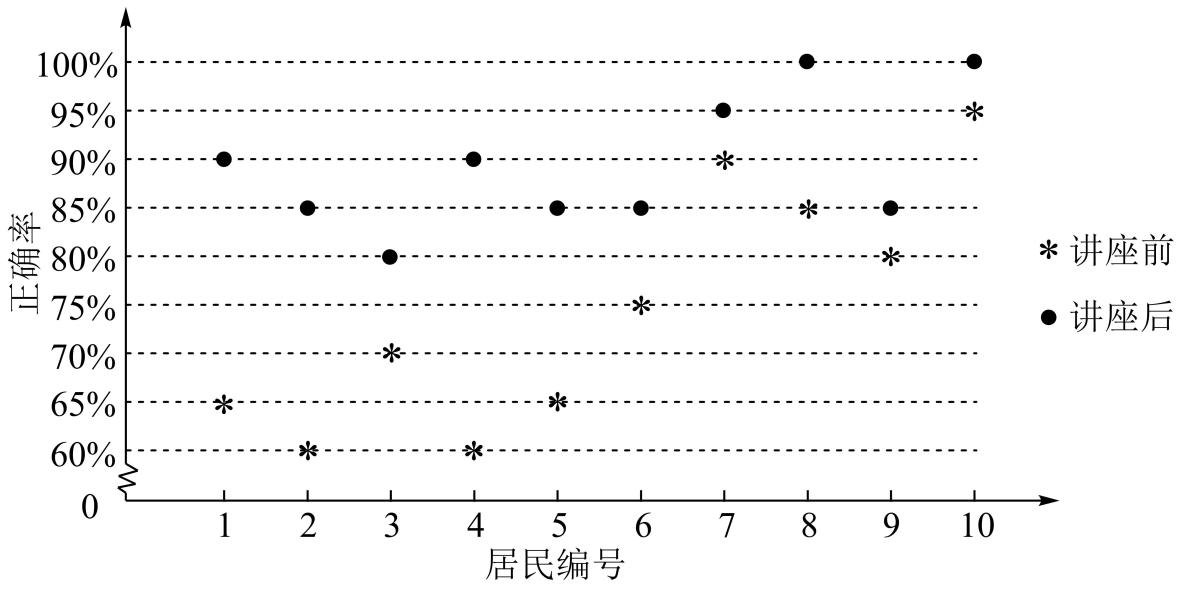
\includegraphics[width=.42\linewidth]{assets/asset-106-01.jpg}
\end{center}
\begin{choices}
  \item 讲座前问卷答题的正确率的中位数小于$70\%$
  \item 讲座后问卷答题的正确率的平均数大于$85\%$
  \item 讲座前问卷答题的正确率的标准差小于讲座后正确率的标准差
  \item 讲座后问卷答题的正确率的极差大于讲座前正确率的极差
\end{choices}
\begin{solution}
\textbf{答案：}B

\textbf{分析：}由图表信息，结合中位数、平均数、标准差、极差的概念，逐项判断即可得解.

\textbf{详解：}讲座前中位数为 $\frac{70\%+75\%}{2} > 70\%$，所以A错；讲座后问卷答题的正确率只有一个是$80\%$，4个$85\%$，剩下全部大于等于$90\%$，所以讲座后问卷答题的正确率的平均数大于$85\%$，所以B对；讲座前问卷答题的正确率更加分散，所以讲座前问卷答题的正确率的标准差大于讲座后正确率的标准差，所以C错；讲座后问卷答题的正确率的极差为$100\%-80\%=20\%$，讲座前问卷答题的正确率的极差为$95\%-60\%=35\%>20\%$，所以D错.故选B.
\end{solution}
\end{question}

\begin{question}[points=5]
\textbf{来源：}2022 年 全国甲卷-理科，第 15 题；次专题：计数原理\par
从正方体的8个顶点中任选4个，则这4个点在同一个平面的概率为．
\fillin[{$\frac{6}{35}$}]
\begin{solution}
\textbf{答案：}$\frac{6}{35}$

\textbf{分析：}根据古典概型的概率公式即可求出.

\textbf{详解：}从正方体的8个顶点中任取4个，有 $n=C_8^4=70$ 个结果，这4个点在同一个平面的有 $m=6+6=12$ 个，故所求概率 $P=\frac{m}{n}=\frac{12}{70}=\frac{6}{35}$. 故答案为 $\frac{6}{35}$.
\end{solution}
\end{question}

\begin{question}[points=12]
\textbf{来源：}2022 年 全国甲卷-理科，第 19 题\par
甲、乙两个学校进行体育比赛，比赛共设三个项目，每个项目胜方得10分，负方得0分，没有平局.三个项目比赛结束后，总得分高的学校获得冠军.已知甲学校在三个项目中获胜的概率分别为0.5, 0.4, 0.8，各项目的比赛结果相互独立.

(1) 求甲学校获得冠军的概率;

(2) 用X表示乙学校的总得分，求X的分布列与期望.
\begin{solution}
\textbf{答案：}(1) $0.6$；(2) 分布列见解析，$E(X)=13$

\textbf{分析：}(1) 设甲在三个项目中获胜的事件依次记为A,B,C，再根据甲获得冠军则至少获胜两个项目，利用互斥事件的概率加法公式以及相互独立事件的乘法公式即可求出. (2) 依题可知，X的可能取值为0,10,20,30，再分别计算出对应的概率，列出分布列，即可求出期望.

\textbf{详解：}(1) 设甲在三个项目中获胜的事件依次记为A,B,C，所以甲学校获得冠军的概率为 $P=P(ABC)+P(A\bar{B}C)+P(\bar{A}BC)+P(AB\bar{C})=0.5\times0.4\times0.8+0.5\times0.4\times0.8+0.5\times0.6\times0.8+0.5\times0.4\times0.2=0.16+0.16+0.24+0.04=0.6$.
(2) 依题可知，X的可能取值为0,10,20,30，所以 $P(X=0)=0.5\times0.4\times0.8=0.16$, $P(X=10)=0.5\times0.4\times0.8+0.5\times0.6\times0.8+0.5\times0.4\times0.2=0.44$, $P(X=20)=0.5\times0.6\times0.8+0.5\times0.4\times0.2+0.5\times0.6\times0.2=0.34$, $P(X=30)=0.5\times0.6\times0.2=0.06$. 即X的分布列为

| X | 0 | 10 | 20 | 30 |
|---|---|----|----|----|
| P | 0.16 | 0.44 | 0.34 | 0.06 |

期望 $E(X)=0\times0.16+10\times0.44+20\times0.34+30\times0.06=13$.
\end{solution}
\end{question}

\begin{question}[points=5]
\textbf{来源：}2022 年 全国甲卷-文科，第 2 题\par
某社区通过公益讲座以普及社区居民的垃圾分类知识．为了解讲座效果，随机抽取10位社区居民，让他们在讲座前和讲座后各回答一份垃圾分类知识问卷，这10位社区居民在讲座前和讲座后问卷答题的正确率如下图：



则

\begin{center}
  
\includegraphics[width=.42\linewidth]{assets/asset-109-01.jpg}
\end{center}
\begin{choices}
  \item A．讲座前问卷答题的正确率的中位数小于70%
  \item B．讲座后问卷答题的正确率的平均数大于85%
  \item C．讲座前问卷答题的正确率的标准差小于讲座后正确率的标准差
  \item D．讲座后问卷答题的正确率的极差大于讲座前正确率的极差
\end{choices}
\begin{solution}
\textbf{答案：}B
\end{solution}
\end{question}

\begin{question}[points=5]
\textbf{来源：}2022 年 全国甲卷-文科，第 6 题\par
从分别写有1，2，3，4，5，6的6张卡片中无放回随机抽取2张，则抽到的2张卡片上的数字之积是4的倍数的概率为
\begin{choices}
  \item $\frac{1}{5}$
  \item $\frac{1}{3}$
  \item $\frac{2}{5}$
  \item $\frac{2}{3}$
\end{choices}
\begin{solution}
\textbf{答案：}C
\end{solution}
\end{question}

\begin{question}[points=12]
\textbf{来源：}2022 年 全国甲卷-文科，第 17 题\par
甲、乙两城之间的长途客车均由 A 和 B 两家公司运营，为了解这两家公司长途客车的运行情况，随机调查了甲、乙两城之间的500个班次，得到下面列联表：



| | 准点班次数 | 未准点班次数 |

| A | 240 | 20 |

| B | 210 | 30 |



（1）根据上表，分别估计这两家公司甲、乙两城之间的长途客车准点的概率；

（2）能否有90%的把握认为甲、乙两城之间的长途客车是否准点与客车所属公司有关？



附：$K^2=\frac{n(ad-bc)^2}{(a+b)(c+d)(a+c)(b+d)}$，



$P(K^2\ge k)$ | 0.100 | 0.050 | 0.010

--- | --- | --- | ---

$k$ | 2.706 | 3.841 | 6.635
\begin{solution}
\textbf{答案：}（1）A 公司准点概率 $\frac{12}{13}$，B 公司准点概率 $\frac{7}{8}$；（2）有90%的把握
\end{solution}
\end{question}

\begin{question}[points=5]
\textbf{来源：}2022 年 全国乙卷-理科，第 10 题\par
某棋手与甲、乙、丙三位棋手各比赛一盘，各盘比赛结果相互独立．已知该棋手与甲、乙、丙比赛获胜的概率分别为$p_1, p_2, p_3$，且$p_3 > p_2 > p_1 > 0$．记该棋手连胜两盘的概率为$p$，则（\qquad）
\begin{choices}
  \item $p$与该棋手和甲、乙、丙的比赛次序无关
  \item 该棋手在第二盘与甲比赛，$p$最大
  \item 该棋手在第二盘与乙比赛，$p$最大
  \item 该棋手在第二盘与丙比赛，$p$最大
\end{choices}
\begin{solution}
\textbf{答案：}D

\textbf{分析：}该棋手连胜两盘，则第二盘为必胜盘.分别求得该棋手在第二盘与甲比赛且连胜两盘的概率$p_{\text{甲}}$；该棋手在第二盘与乙比赛且连胜两盘的概率$p_{\text{乙}}$；该棋手在第二盘与丙比赛且连胜两盘的概率$p_{\text{丙}}$.并对三者进行比较即可解决

\textbf{详解：}该棋手连胜两盘，则第二盘为必胜盘，记该棋手在第二盘与甲比赛，且连胜两盘的概率为$p_{\text{甲}}$则$p_{\text{甲}} = 2(1-p_2)p_1p_3 + 2p_2p_1(1-p_3) = 2p_1(p_2+p_3) - 4p_1p_2p_3$记该棋手在第二盘与乙比赛，且连胜两盘的概率为$p_{\text{乙}}$则$p_{\text{乙}} = 2(1-p_1)p_2p_3 + 2p_1p_2(1-p_3) = 2p_2(p_1+p_3) - 4p_1p_2p_3$记该棋手在第二盘与丙比赛，且连胜两盘的概率为$p_{\text{丙}}$则$p_{\text{丙}} = 2(1-p_1)p_3p_2 + 2p_1p_3(1-p_2) = 2p_3(p_1+p_2) - 4p_1p_2p_3$则$p_{\text{甲}} - p_{\text{乙}} = 2p_1(p_2+p_3) - 4p_1p_2p_3 - [2p_2(p_1+p_3) - 4p_1p_2p_3] = 2(p_1-p_2)p_3 < 0$\\$p_{\text{乙}} - p_{\text{丙}} = 2p_2(p_1+p_3) - 4p_1p_2p_3 - [2p_3(p_1+p_2) - 4p_1p_2p_3] = 2(p_2-p_3)p_1 < 0$即$p_{\text{甲}} < p_{\text{乙}}$，$p_{\text{乙}} < p_{\text{丙}}$，则该棋手在第二盘与丙比赛，$p$最大.
\end{solution}
\end{question}

\begin{question}[points=5]
\textbf{来源：}2022 年 全国乙卷-理科，第 13 题；次专题：计数原理\par
从甲、乙等5名同学中随机选3名参加社区服务工作，则甲、乙都入选的概率为．
\fillin[{$\frac{3}{10}$}]
\begin{solution}
\textbf{答案：}$\frac{3}{10}$

\textbf{分析：}根据古典概型计算即可

\textbf{详解：}从5名同学中随机选3名的方法数为$\mathrm{C}_5^3 = 10$甲、乙都入选的方法数为$\mathrm{C}_3^1 = 3$，所以甲、乙都入选的概率$P = \frac{3}{10}$
\end{solution}
\end{question}

\begin{question}[points=12]
\textbf{来源：}2022 年 全国乙卷-理科，第 19 题\par
某地经过多年的环境治理，已将荒山改造成了绿水青山．为估计一林区某种树木的总材积量，随机选取了10棵这种树木，测量每棵树的根部横截面积（单位：$m^2$）和材积量（单位：$m^3$），得到如下数据：



| 样本号$i$ | 1 | 2 | 3 | 4 | 5 | 6 | 7 | 8 | 9 | 10 | 总和 |

|-----------|---|---|---|---|---|---|---|---|---|---|------|

| 根部横截面积$x_i$ | 0.04 | 0.06 | 0.04 | 0.08 | 0.08 | 0.05 | 0.05 | 0.07 | 0.07 | 0.06 | 0.6 |

| 材积量$y_i$ | 0.25 | 0.40 | 0.22 | 0.54 | 0.51 | 0.34 | 0.36 | 0.46 | 0.42 | 0.40 | 3.9 |



并计算得$\sum\limits_{i=1}^{10} x_i^2 = 0.038, \sum\limits_{i=1}^{10} y_i^2 = 1.6158, \sum\limits_{i=1}^{10} x_i y_i = 0.2474$．

(1)估计该林区这种树木平均一棵的根部横截面积与平均一棵的材积量；

(2)求该林区这种树木的根部横截面积与材积量的样本相关系数（精确到0.01）；

(3)现测量了该林区所有这种树木的根部横截面积，并得到所有这种树木的根部横截面积总和为$186m^2$．已知树木的材积量与其根部横截面积近似成正比．利用以上数据给出该林区这种树木的总材积量的估计值．

附：相关系数$r=\frac{\sum\limits_{i=1}^n (x_i-\bar{x})(y_i-\bar{y})}{\sqrt{\sum\limits_{i=1}^n (x_i-\bar{x})^2 \sum\limits_{i=1}^n (y_i-\bar{y})^2}}$，$\sqrt{1.896} \approx 1.377$．
\begin{solution}
\textbf{答案：}(1) $0.06m^2$；$0.39m^3$
(2) $0.97$
(3) $1209m^3$

\textbf{分析：}(1)计算出样本的一棵根部横截面积的平均值及一棵材积量平均值，即可估计该林区这种树木平均一棵的根部横截面积与平均一棵的材积量；(2)代入题给相关系数公式去计算即可求得样本的相关系数值；(3)依据树木的材积量与其根部横截面积近似成正比，列方程即可求得该林区这种树木的总材积量的估计值．

\textbf{详解：}【小问1详解】样本中10棵这种树木的根部横截面积的平均值$\bar{x} = \frac{0.6}{10} = 0.06$样本中10棵这种树木的材积量的平均值$\bar{y} = \frac{3.9}{10} = 0.39$据此可估计该林区这种树木平均一棵的根部横截面积为$0.06m^2$，平均一棵的材积量为$0.39m^3$\\【小问2详解】\\$r = \frac{\sum\limits_{i=1}^{10} (x_i-\bar{x})(y_i-\bar{y})}{\sqrt{\sum\limits_{i=1}^{10} (x_i-\bar{x})^2 \sum\limits_{i=1}^{10} (y_i-\bar{y})^2}} = \frac{\sum\limits_{i=1}^{10} x_i y_i - 10\bar{x}\bar{y}}{\sqrt{(\sum\limits_{i=1}^{10} x_i^2 - 10\bar{x}^2)(\sum\limits_{i=1}^{10} y_i^2 - 10\bar{y}^2)}}$\\$= \frac{0.2474 - 10\times0.06\times0.39}{\sqrt{(0.038 - 10\times0.06^2)(1.6158 - 10\times0.39^2)}} = \frac{0.0134}{\sqrt{0.0001896}} \approx \frac{0.0134}{0.01377} \approx 0.97$则$r \approx 0.97$\\【小问3详解】设该林区这种树木的总材积量的估计值为$Y\,m^3$，又已知树木的材积量与其根部横截面积近似成正比，可得$\frac{0.06}{0.39} = \frac{186}{Y}$，解之得$Y=1209m^3$．则该林区这种树木的总材积量估计为$1209m^3$
\end{solution}
\end{question}

\begin{question}[points=5]
\textbf{来源：}2022 年 全国乙卷-文科，第 4 题\par
分别统计了甲、乙两位同学16周的各周课外体育运动时长（单位：h），得如下茎叶图：



则下列结论中错误的是
\begin{choices}
  \item 甲同学周课外体育运动时长的样本中位数为7.4
  \item 乙同学周课外体育运动时长的样本平均数大于8
  \item 甲同学周课外体育运动时长大于8的概率的估计值大于0.4
  \item 乙同学周课外体育运动时长大于8的概率的估计值大于0.6
\end{choices}
\begin{solution}
\textbf{答案：}C

\textbf{分析：}结合茎叶图、中位数、平均数、古典概型等知识确定正确答案.

\textbf{详解：}对于A，甲同学样本中位数为 $\frac{7.3+7.5}{2}=7.4$, 正确. 对于B，乙同学平均数为 $8.50625>8$, 正确. 对于C，甲同学时长大于8的概率估计值为 $\frac{6}{16}=0.375<0.4$, 错误. 对于D，乙同学时长大于8的概率估计值为 $\frac{13}{16}=0.8125>0.6$, 正确.
\end{solution}
\end{question}

\begin{question}[points=5]
\textbf{来源：}2022 年 全国乙卷-文科，第 14 题\par
从甲、乙等5名同学中随机选3名参加社区服务工作，则甲、乙都入选的概率为.
\fillin[{$\frac{3}{10}$}]
\begin{solution}
\textbf{答案：}$\frac{3}{10}$

\textbf{分析：}根据古典概型计算即可.

\textbf{详解：}从5名同学中选3名，共有 $C_5^3=10$ 种选法，甲、乙都入选的选法有 $C_3^1=3$ 种，所以概率为 $\frac{3}{10}$.
\end{solution}
\end{question}

\begin{question}[points=12]
\textbf{来源：}2022 年 全国乙卷-文科，第 19 题\par
某地经过多年的环境治理，已将荒山改造成了绿水青山．为估计一林区某种树木的总材积量，随机选取了10棵这种树木，测量每棵树的根部横截面积（单位：$m^2$）和材积量（单位：$m^3$），得到如下数据：

\begin{tabular}{c|cccccccccc|c}

样本号 $i$ & 1 & 2 & 3 & 4 & 5 & 6 & 7 & 8 & 9 & 10 & 总和 \\ \hline

根部横截面积 $x_i$ & 0.04 & 0.06 & 0.04 & 0.08 & 0.08 & 0.05 & 0.05 & 0.07 & 0.07 & 0.06 & 0.6 \\

材积量 $y_i$ & 0.25 & 0.40 & 0.22 & 0.54 & 0.51 & 0.34 & 0.36 & 0.46 & 0.42 & 0.40 & 3.9 \\

\end{tabular}

并计算得 $\sum_{i=1}^{10} x_i^2 = 0.038$, $\sum_{i=1}^{10} y_i^2 = 1.6158$, $\sum_{i=1}^{10} x_i y_i = 0.2474$.

(1) 估计该林区这种树木平均一棵的根部横截面积与平均一棵的材积量；

(2) 求该林区这种树木的根部横截面积与材积量的样本相关系数（精确到0.01）；

(3) 现测量了该林区所有这种树木的根部横截面积，并得到所有这种树木的根部横截面积总和为 $186 m^2$．已知树木的材积量与其根部横截面积近似成正比．利用以上数据给出该林区这种树木的总材积量的估计值．

附：相关系数 $r = \frac{\sum_{i=1}^{n}(x_i-\bar{x})(y_i-\bar{y})}{\sqrt{\sum_{i=1}^{n}(x_i-\bar{x})^2 \sum_{i=1}^{n}(y_i-\bar{y})^2}}$, $\sqrt{1.896}\approx1.377$.
\begin{solution}
\textbf{答案：}(1) $0.06m^2$, $0.39m^3$; (2) $0.97$; (3) $1209m^3$.

\textbf{分析：}计算样本平均值得估计值；代入相关系数公式计算；利用正比例关系求总材积量.

\textbf{详解：}(1) $\bar{x}=0.06$, $\bar{y}=0.39$.
(2) $r = \frac{0.2474-10\times0.06\times0.39}{\sqrt{(0.038-10\times0.06^2)(1.6158-10\times0.39^2)}} = \frac{0.0134}{\sqrt{0.0001896}} \approx \frac{0.0134}{0.01377} \approx 0.97$.
(3) 设总材积量为 $Y$, 由 $\frac{0.06}{0.39}=\frac{186}{Y}$ 得 $Y=1209m^3$.
\end{solution}
\end{question}

\begin{question}[points=5]
\textbf{来源：}2022 年 上海卷，第 8 题\par
为了检测学生的身体素质指标，从游泳类 1 项，球类 3 项，田径类 4 项共 8 项项目中随机抽取 4 项进行检测，则每一类都被抽到的概率为 ．
\fillin[{$\frac{3}{7}$}]
\begin{solution}
\textbf{答案：}$\frac{3}{7}$

\textbf{分析：}利用古典概率的计算公式，计算求得结果．

\textbf{详解：}解：从游泳类 1 项，球类 3 项，田径类 4 项共 8 项项目中随机抽取 4 项进行检测，则每一类都被抽到的方法共有$C_1^1\cdot C_3^1\cdot C_4^2 + C_1^1\cdot C_3^2\cdot C_4^1$种，而所有的抽取方法共有$C_8^4$种，故每一类都被抽到的概率为$\frac{C_1^1\cdot C_3^1\cdot C_4^2 + C_1^1\cdot C_3^2\cdot C_4^1}{C_8^4}=\frac{30}{70}=\frac{3}{7}$．故答案为：$\frac{3}{7}$．
\end{solution}
\end{question}

\begin{question}[points=5]
\textbf{来源：}2022 年 天津卷，第 4 题\par
为研究某药品的疗效，选取若干名志愿者进行临床试验，所有志愿者的舒张压数据（单位：kPa）的分组区间为 $[12,13),[13,14),[14,15),[15,16),[16,17]$ ，将其按从左到右的顺序分别编号为第一组，第二组，…，第五组，右图是根据试验数据制成的频率分布直方图．已知第一组与第二组共有 20 人，第三组中没有疗效的有 6 人，则第三组中有疗效的人数为（   ）

\begin{center}
  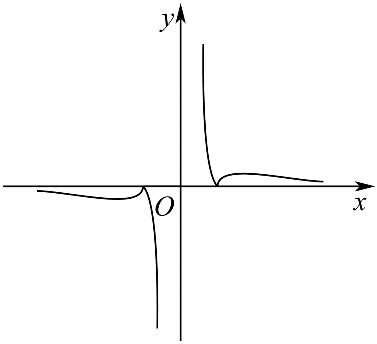
\includegraphics[width=.42\linewidth]{assets/asset-119-01.jpg}
\end{center}
\begin{choices}
  \item 8
  \item 12
  \item 16
  \item 18
\end{choices}
\begin{solution}
\textbf{答案：}12

\textbf{分析：}志愿者的总人数为 $\frac{20}{(0.24+0.16)\times 1}=50$，所以第三组人数为 $50\times 0.36=18$，有疗效的人数为 $18-6=12$.
\end{solution}
\end{question}

\begin{question}[points=5]
\textbf{来源：}2022 年 天津卷，第 13 题\par
52 张扑克牌，没有大小王，无放回地抽取两次，则两次都抽到 A 的概率为；已知第一次抽到的是 A，则第二次抽取 A 的概率为
\fillin[{$\frac{1}{221}$ 和 $\frac{1}{17}$}]
\begin{solution}
\textbf{答案：}$\frac{1}{221}$ 和 $\frac{1}{17}$

\textbf{分析：}设第一次抽到 A 的事件为 $B$，第二次抽到 A 的事件为 $C$，则 $P(BC)=\frac{4}{52}\times\frac{3}{51}=\frac{1}{221}$，$P(B)=\frac{4}{52}=\frac{1}{13}$，$P(C|B)=\frac{P(BC)}{P(B)}=\frac{1}{221}\div\frac{1}{13}=\frac{1}{17}$.
\end{solution}
\end{question}

\begin{question}[points=5]
\textbf{来源：}2022 年 新高考II卷，第 13 题\par
已知随机变量$X$服从正态分布$N(2,\sigma^2)$，且$P(2<X\leq 2.5)=0.36$，则$P(X>2.5)=$.
\fillin[{$0.14$}]
\begin{solution}
\textbf{答案：}$0.14$

\textbf{分析：}根据正态分布曲线的性质即可解出.

\textbf{详解：}因为$X\sim N(2,\sigma^2)$，所以$P(X<2)=P(X>2)=0.5$，因此$P(X>2.5)=P(X>2)-P(2<X\leq 2.5)=0.5-0.36=0.14$．故答案为$0.14$．
\end{solution}
\end{question}

\begin{question}[points=12]
\textbf{来源：}2022 年 新高考II卷，第 19 题\par
在某地区进行流行病学调查，随机调查了100位某种疾病患者的年龄，得到如下的样本数据的频率分布直方图：

(1)估计该地区这种疾病患者的平均年龄（同一组中的数据用该组区间的中点值为代表）；

(2)估计该地区一位这种疾病患者的年龄位于区间$[20,70)$的概率；

(3)已知该地区这种疾病的患病率为$0.1\%$，该地区年龄位于区间$[40,50)$的人口占该地区总人口的$16\%$．从该地区中任选一人，若此人的年龄位于区间$[40,50)$，求此人患这种疾病的概率．（以样本数据中患者的年龄位于各区间的频率作为患者的年龄位于该区间的概率，精确到$0.0001$）.

\begin{center}
  
\includegraphics[width=.42\linewidth]{assets/asset-122-01.jpg}
\end{center}
\begin{solution}
\textbf{答案：}(1)$47.9$岁；(2)$0.89$；(3)$0.0014$

\textbf{分析：}(1)根据平均值等于各矩形的面积乘以对应区间的中点值的和即可求出；(2)设$A=\{$一人患这种疾病的年龄在区间$[20,70)\}$，根据对立事件的概率公式$P(A)=1-P(\overline{A})$即可解出；(3)根据条件概率公式即可求出.

\textbf{详解：}（1）平均年龄$\bar{x}=(5\times0.001+15\times0.002+25\times0.012+35\times0.017+45\times0.023+55\times0.020+65\times0.017+75\times0.006+85\times0.002)\times10=47.9$（岁）．
（2）设$A=\{$一人患这种疾病的年龄在区间$[20,70)\}$，所以$P(A)=1-P(\overline{A})=1-(0.001+0.002+0.006+0.002)\times10=1-0.11=0.89$．
（3）设$B=$“任选一人年龄位于区间$[40,50)$”，$C=$“从该地区中任选一人患这种疾病”，则由已知得：$P(B)=16\%=0.16,P(C)=0.1\%=0.001,P(B|C)=0.023\times10=0.23$，则由条件概率公式可得从该地区中任选一人，若此人的年龄位于区间$[40,50)$，此人患这种疾病的概率为$P(C|B)=\dfrac{P(BC)}{P(B)}=\dfrac{P(C)P(B|C)}{P(B)}=\dfrac{0.001\times0.23}{0.16}=0.0014375\approx 0.0014$．
\end{solution}
\end{question}

\begin{question}[points=5]
\textbf{来源：}2022 年 新高考I卷，第 5 题\par
从 2 至 8 的 7 个整数中随机取 2 个不同的数, 则这 2 个数互质的概率为
\begin{choices}
  \item $\frac{1}{6}$
  \item $\frac{1}{3}$
  \item $\frac{1}{2}$
  \item $\frac{2}{3}$
\end{choices}
\begin{solution}
\textbf{答案：}D

\textbf{分析：}由古典概型概率公式结合组合、列举法即可得解.

\textbf{详解：}从 2 至 8 的 7 个整数中随机取 2 个不同的数, 共有 $C_7^2 = 21$ 种不同的取法. 若两数不互质, 不同的取法有: $(2,4)$, $(2,6)$, $(2,8)$, $(3,6)$, $(4,6)$, $(4,8)$, $(6,8)$, 共 7 种. 故所求概率 $P = \frac{21 - 7}{21} = \frac{2}{3}$.
\end{solution}
\end{question}

\begin{question}[points=12]
\textbf{来源：}2022 年 新高考I卷，第 20 题\par
一医疗团队为研究某地的一种地方性疾病与当地居民的卫生习惯（卫生习惯分为良好和不够良好两类）的关系, 在已患该疾病的病例中随机调查了 100 例（称为病例组）, 同时在未患该疾病的人群中随机调查了 100 人（称为对照组）, 得到如下数据：

\begin{center}\begin{tabular}{c|c|c}

 & 不够良好 & 良好 \\ \hline

病例组 & 40 & 60 \\

对照组 & 10 & 90 \\

\end{tabular}\end{center}

(1) 能否有 99% 的把握认为患该疾病群体与未患该疾病群体的卫生习惯有差异？

(2) 从该地的人群中任选一人, $A$ 表示事件“选到的人卫生习惯不够良好”, $B$ 表示事件“选到的人患有该疾病”. $\frac{P(B|A)}{P(\bar{B}|A)}$ 与 $\frac{P(B|\bar{A})}{P(\bar{B}|\bar{A})}$ 的比值是卫生习惯不够良好对患该疾病风险程度的一项度量指标, 记该指标为 $R$.

(i) 证明: $R = \frac{P(A|B)}{P(\bar{A}|B)} \cdot \frac{P(\bar{A}|\bar{B})}{P(A|\bar{B})}$;

(ii) 利用该调查数据, 给出 $P(A|B)$, $P(A|\bar{B})$ 的估计值, 并利用 (i) 的结果给出 $R$ 的估计值.

附: $K^2 = \frac{n(ad - bc)^2}{(a+b)(c+d)(a+c)(b+d)}$, $\begin{array}{c|ccc} P(K^2 \ge k) & 0.050 & 0.010 & 0.001 \\ \hline k & 3.841 & 6.635 & 10.828 \end{array}$
\begin{solution}
\textbf{答案：}(1) 有 99% 的把握; (2)(i) 见解析; (ii) $R = 6$

\textbf{分析：}(1) 由所给数据结合公式求出 $K^2$ 的值, 将其与临界值比较大小, 由此确定是否有 99% 的把握认为患该疾病群体与未患该疾病群体的卫生习惯有差异. (2)(i) 根据定义结合条件概率公式即可完成证明; (ii) 根据 (i) 结合已知数据求 $R$.

\textbf{详解：}(1) 由已知 $K^2 = \frac{200 \times (40 \times 90 - 60 \times 10)^2}{50 \times 150 \times 100 \times 100} = 24$. 又 $P(K^2 \ge 6.635) = 0.01$, $24 > 6.635$, 所以有 99% 的把握认为患该疾病群体与未患该疾病群体的卫生习惯有差异.
(2)(i) $R = \frac{P(B|A)}{P(\bar{B}|A)} \cdot \frac{P(\bar{B}|\bar{A})}{P(B|\bar{A})} = \frac{P(AB)}{P(A)} \cdot \frac{P(\bar{A})}{P(\bar{A}B)} \cdot \frac{P(\bar{B}\bar{A})}{P(\bar{A})} \cdot \frac{P(A)}{P(A\bar{B})} = \frac{P(AB)}{P(\bar{A}B)} \cdot \frac{P(\bar{A}\bar{B})}{P(A\bar{B})} = \frac{P(A|B)}{P(\bar{A}|B)} \cdot \frac{P(\bar{A}|\bar{B})}{P(A|\bar{B})}$.
(ii) 由已知 $P(A|B) = \frac{40}{100} = \frac{2}{5}$, $P(A|\bar{B}) = \frac{10}{100} = \frac{1}{10}$, $P(\bar{A}|B) = \frac{60}{100} = \frac{3}{5}$, $P(\bar{A}|\bar{B}) = \frac{90}{100} = \frac{9}{10}$. 所以 $R = \frac{P(A|B)}{P(\bar{A}|B)} \cdot \frac{P(\bar{A}|\bar{B})}{P(A|\bar{B})} = \frac{2/5}{3/5} \times \frac{9/10}{1/10} = \frac{2}{3} \times 9 = 6$.
\end{solution}
\end{question}

\begin{question}[points=6]
\textbf{来源：}2022 年 浙江卷，第 15 题\par
现有7张卡片，分别写上数字1,2,2,3,4,5,6．从这7张卡片中随机抽取3张，记所抽取卡片上数字的最小值为 $\xi$，则 $P(\xi=2) =$ ，$E(\xi) =$ ．
\fillin[{$\dfrac{16}{35}$；$\dfrac{12}{7}$}]
\begin{solution}
\textbf{答案：}$\dfrac{16}{35}$；$\dfrac{12}{7}$

\textbf{分析：}利用古典概型概率公式求 $P(\xi=2)$，由条件求 $\xi$ 分布列，再由期望公式求其期望.

\textbf{详解：}从7张中任取3张共有 $C_7^3=35$ 种取法，$\xi=2$ 时，抽取的卡片中不含1且至少有一张2，取法有 $C_4^1 + C_2^1 C_4^2 = 4+12=16$，所以 $P(\xi=2)=\frac{16}{35}$；$\xi$ 的取值为1,2,3,4，$P(\xi=1)=\frac{C_6^2}{C_7^3}=\frac{15}{35}$，$P(\xi=2)=\frac{16}{35}$，$P(\xi=3)=\frac{C_3^2}{C_7^3}=\frac{3}{35}$，$P(\xi=4)=\frac{1}{35}$，所以 $E(\xi)=1\times\frac{15}{35}+2\times\frac{16}{35}+3\times\frac{3}{35}+4\times\frac{1}{35}=\frac{12}{7}$.
\end{solution}
\end{question}

\section*{2023 年}

\begin{question}[points=13]
\textbf{来源：}2023 年 北京卷，第 18 题\par
为研究某种农产品价格变化的规律，收集得到了该农产品连续40天的价格变化数据，如下表所示．在描述价格变化时，用“+”表示“上涨”，即当天价格比前一天价格高；用“-”表示“下跌”，即当天价格比前一天价格低；用“0”表示“不变”，即当天价格与前一天价格相同．



时段                                                  价格变化



第1天到第20天     -  +  +  0  -  -  -  +  +  0  +  0  -  -  +  -  +  0  0  +



第21天到第40天     0  +  +  0  -  -  -  +  +  0  +  0  +  -  -  -  +  0  -  +



用频率估计概率．

（1）试估计该农产品价格“上涨”的概率；

（2）假设该农产品每天的价格变化是相互独立的．在未来的日子里任取4天，试估计该农产品价格在这4天中2天“上涨”、1天“下跌”、1天“不变”的概率；

（3）假设该农产品每天的价格变化只受前一天价格变化的影响．判断第41天该农产品价格“上涨”“下跌”和“不变”的概率估计值哪个最大．（结论不要求证明）
\begin{solution}
\textbf{答案：}（1）0.4 （2）0.168 （3）不变

\textbf{分析：}（1）计算表格中的+的次数，然后根据古典概型进行计算；（2）分别计算出表格中上涨，不变，下跌的概率后进行计算；（3）通过统计表格中前一次上涨，后一次发生的各种情况进行推断第41天的情况.

\textbf{详解：}（1）根据表格数据可以看出，40天里，有16个+，也就是有16天是上涨的，根据古典概型的计算公式，农产品价格上涨的概率为 $\frac{16}{40}=0.4$。
（2）在这40天里，有16天上涨，14天下跌，10天不变，也就是上涨、下跌、不变的概率分别是0.4，0.35，0.25。于是未来任取4天，2天上涨，1天下跌，1天不变的概率是 $C_4^2 \times 0.4^2 \times C_2^1 \times 0.35 \times 0.25 = 6 \times 0.16 \times 2 \times 0.35 \times 0.25 = 0.168$。
（3）由于第40天处于上涨状态，从前39次的15次上涨进行分析，上涨后下一次仍上涨的有4次，不变的有9次，下跌的有2次，因此估计第41次不变的概率最大。
\end{solution}
\end{question}

\begin{question}[points=5]
\textbf{来源：}2023 年 全国甲卷-理科，第 6 题\par
某地的中学生中有 $60\%$ 的同学爱好滑冰，$50\%$ 的同学爱好滑雪，$70\%$ 的同学爱好滑冰或爱好滑雪．在该地的中学生中随机调查一位同学，若该同学爱好滑雪，则该同学也爱好滑冰的概率为（                                                        ）
\begin{choices}
  \item $0.8$
  \item $0.6$
  \item $0.5$
  \item $0.4$
\end{choices}
\begin{solution}
\textbf{答案：}A

\textbf{分析：}先算出同时爱好两项的概率，利用条件概率的知识求解．

\textbf{详解：}同时爱好两项的概率为 $0.5 + 0.6 - 0.7 = 0.4$，记“该同学爱好滑雪”为事件 $A$，记“该同学爱好滑冰”为事件 $B$，则 $P(A)=0.5$，$P(AB)=0.4$，所以 $P(B|A) = \frac{P(AB)}{P(A)} = \frac{0.4}{0.5} = 0.8$．
\end{solution}
\end{question}

\begin{question}[points=12]
\textbf{来源：}2023 年 全国甲卷-理科，第 19 题\par
一项试验旨在研究臭氧效应．实验方案如下：选 40 只小白鼠，随机地将其中 20 只分配到实验组，另外 20 只分配到对照组，实验组的小白鼠饲养在高浓度臭氧环境，对照组的小白鼠饲养在正常环境，一段时间后统计每只小白鼠体重的增加量（单位：g）．

（1）设 $X$ 表示指定的两只小白鼠中分配到对照组的只数，求 $X$ 的分布列和数学期望；

（2）实验结果如下：

对照组的小白鼠体重的增加量从小到大排序为：

15.2 18.8 20.2 21.3 22.5 23.2 25.8 26.5 27.5 30.1

32.6 34.3 34.8 35.6 35.6 35.8 36.2 37.3 40.5 43.2

实验组的小白鼠体重的增加量从小到大排序为：

7.8 9.2 11.4 12.4 13.2 15.5 16.5 18.0 18.8 19.2

19.8 20.2 21.6 22.8 23.6 23.9 25.1 28.2 32.3 36.5

（i）求 40 只小鼠体重的增加量的中位数 $m$，再分别统计两样本中小于 $m$ 与不小于 $m$ 的数据的个数，完成如下列联表：

$\begin{array}{c|c|c} 

 & <m & \ge m \\ \hline

\text{对照组} & & \\ \hline

\text{实验组} & & \\ \hline

\end{array}$

（ii）根据（i）中的列联表，能否有 95\% 的把握认为小白鼠在高浓度臭氧环境中与正常环境中体重的增加量有差异．

附：$K^2 = \frac{n(ad-bc)^2}{(a+b)(c+d)(a+c)(b+d)}$，

$\begin{array}{c|ccc} 

P(K^2\ge k_0) & 0.100 & 0.050 & 0.010 \\ \hline

k_0 & 2.706 & 3.841 & 6.635 \\ \hline

\end{array}$
\begin{solution}
\textbf{答案：}（1）分布列见解析，$E(X)=1$；（2）（i）$m=23.4$，列联表见解析，（ii）能

\textbf{分析：}（1）利用超几何分布的知识即可求得分布列及数学期望；（2）（i）根据中位数的定义即可求得 $m=23.4$，从而求得列联表；（ii）利用独立性检验的卡方计算进行检验，即可得解．

\textbf{详解：}（1）依题意，$X$ 的可能取值为 $0,1,2$，则 $P(X=0) = \frac{C_{20}^0 C_{20}^2}{C_{40}^2} = \frac{19}{78}$，$P(X=1) = \frac{C_{20}^1 C_{20}^1}{C_{40}^2} = \frac{20}{39}$，$P(X=2) = \frac{C_{20}^2 C_{20}^0}{C_{40}^2} = \frac{19}{78}$，所以 $X$ 的分布列为：
$\begin{array}{c|ccc} 
X & 0 & 1 & 2 \\ \hline
P & \frac{19}{78} & \frac{20}{39} & \frac{19}{78} \\ \hline
\end{array}$
故 $E(X) = 0\times\frac{19}{78} + 1\times\frac{20}{39} + 2\times\frac{19}{78} = 1$．
（2）（i）依题意，可知这 40 只小白鼠体重增量的中位数是将两组数据合在一起，从小到大排后第 20 位与第 21 位数据的平均数，观察数据可得第 20 位为 23.2，第 21 位数据为 23.6，所以 $m = \frac{23.2+23.6}{2} = 23.4$，故列联表为：
$\begin{array}{c|c|c|c} 
 & <m & \ge m & \text{合计} \\ \hline
\text{对照组} & 6 & 14 & 20 \\ \hline
\text{实验组} & 14 & 6 & 20 \\ \hline
\text{合计} & 20 & 20 & 40 \\ \hline
\end{array}$
（ii）由（i）可得，$K^2 = \frac{40\times(6\times6-14\times14)^2}{20\times20\times20\times20} = 6.400 > 3.841$，所以能有 95% 的把握认为小白鼠在高浓度臭氧环境中与正常环境中体重的增加量有差异．
\end{solution}
\end{question}

\begin{question}[points=5]
\textbf{来源：}2023 年 全国甲卷-文科，第 4 题\par
某校文艺部有4名学生，其中高一、高二年级各2名．从这4名学生中随机选2名组织校文艺汇演，则这2名学生来自不同年级的概率为（    ）
\begin{choices}
  \item $\frac{1}{6}$
  \item $\frac{1}{3}$
  \item $\frac{1}{2}$
  \item $\frac{2}{3}$
\end{choices}
\begin{solution}
\textbf{答案：}D

\textbf{分析：}利用古典概率的概率公式，结合组合的知识即可得解.

\textbf{详解：}依题意，从这4名学生中随机选2名组织校文艺汇演，总的基本事件有 $\mathrm{C}_4^2 = 6$ 件，其中这2名学生来自不同年级的基本事件有 $\mathrm{C}_2^1 \mathrm{C}_2^1 = 4$，所以这2名学生来自不同年级的概率为 $\frac{4}{6} = \frac{2}{3}$，故选D.
\end{solution}
\end{question}

\begin{question}
\textbf{来源：}2023 年 全国甲卷-文科，第 19 题\par
一项试验旨在研究臭氧效应，试验方案如下：选40只小白鼠，随机地将其中20只分配到试验组，另外20只分配到对照组，试验组的小白鼠饲养在高浓度臭氧环境，对照组的小白鼠饲养在正常环境，一段时间后统计每只小白鼠体重的增加量（单位：g）．试验结果如下：

对照组的小白鼠体重的增加量从小到大排序为

15.2 18.8 20.2 21.3 22.5 23.2 25.8 26.5 27.5 30.1

32.6 34.3 34.8 35.6 35.6 35.8 36.2 37.3 40.5 43.2

试验组的小白鼠体重的增加量从小到大排序为

7.8 9.2 11.4 12.4 13.2 15.5 16.5 18.0 18.8 19.2

19.8 20.2 21.6 22.8 23.6 23.9 25.1 28.2 32.3 36.5

（1）计算试验组的样本平均数；

（2）（ⅰ）求40只小白鼠体重的增加量的中位数 $m$，再分别统计两样本中小于 $m$ 与不小于 $m$ 的数据的个数，完成如下列联表

$\begin{array}{c|cc} & <m & \ge m \\ \hline \text{对照组} & & \\ \text{试验组} & & \\ \end{array}$

（ⅱ）根据（i）中的列联表，能否有95%的把握认为小白鼠在高浓度臭氧环境中与在正常环境中体重的增加量有差异？

附：$K^2=\frac{n(ad-bc)^2}{(a+b)(c+d)(a+c)(b+d)}$，$P(K^2\ge k)$ 0.100 0.050 0.010，$k$ 2.706 3.841 6.635
\begin{solution}
\textbf{答案：}（1）19.8；（2）（i）$m=23.4$，列联表见解析；（ii）能有95%的把握认为有差异

\textbf{分析：}（1）直接根据均值定义求解；（2）（i）根据中位数的定义即可求得 $m=23.4$，从而求得列联表；（ii）利用独立性检验的卡方计算进行检验，即可得解.

\textbf{详解：}（1）试验组样本平均数为：$\frac{1}{20}(7.8+9.2+11.4+12.4+13.2+15.5+16.5+18.0+18.8+19.2+19.8+20.2+21.6+22.8+23.6+23.9+25.1+28.2+32.3+36.5)=\frac{396}{20}=19.8$．
（2）（i）依题意，可知这40只小鼠体重的中位数是将两组数据合在一起，从小到大排后第20位与第21位数据的平均数，由原数据可得第11位数据为18.8，后续依次为19.2,19.8,20.2,20.2,21.3,21.6,22.5,22.8,23.2,23.6,$\cdots$，故第20位为23.2，第21位数据为23.6，所以 $m=\frac{23.2+23.6}{2}=23.4$，故列联表为：
$\begin{array}{c|cc|c} & <m & \ge m & \text{合计} \\ \hline \text{对照组} & 6 & 14 & 20 \\ \text{试验组} & 14 & 6 & 20 \\ \hline \text{合计} & 20 & 20 & 40 \end{array}$
（ii）由（i）可得，$K^2=\frac{40\times(6\times6-14\times14)^2}{20\times20\times20\times20}=6.400>3.841$，所以能有95%的把握认为小白鼠在高浓度臭氧环境中与在正常环境中体重的增加量有差异.
\end{solution}
\end{question}

\begin{question}[points=5]
\textbf{来源：}2023 年 全国乙卷-理科，第 5 题\par
设 $O$ 为平面坐标系的坐标原点，在区域 $\{(x,y)|1\le x^{2}+y^{2}\le 4\}$ 内随机取一点，记该点为 $A$，则直线 $OA$ 的倾斜角不大于 $\frac{\pi}{4}$ 的概率为（ ）
\begin{choices}
  \item $\frac{1}{8}$
  \item $\frac{1}{6}$
  \item $\frac{1}{4}$
  \item $\frac{1}{2}$
\end{choices}
\begin{solution}
\textbf{答案：}$\frac{1}{4}$

\textbf{分析：}根据题意分析区域的几何意义，结合几何概型运算求解.

\textbf{详解：}因为区域 $\{(x,y)|1\le x^{2}+y^{2}\le 4\}$ 表示以 $O(0,0)$ 为圆心，外圆半径 $R=2$，内圆半径 $r=1$ 的圆环，则直线 $OA$ 的倾斜角不大于 $\frac{\pi}{4}$ 的部分如阴影所示，在第一象限部分对应的圆心角 $\angle MON=\frac{\pi}{4}$，结合对称性可得所求概率 $P=\frac{2\times \frac{\pi}{4}}{2\pi}=\frac{1}{4}$.
\end{solution}
\end{question}

\begin{question}[points=12]
\textbf{来源：}2023 年 全国乙卷-理科，第 17 题\par
某厂为比较甲乙两种工艺对橡胶产品伸缩率的处理效应，进行10次配对试验，每次配对试验选用材质相同的两个橡胶产品，随机地选其中一个用甲工艺处理，另一个用乙工艺处理，测量处理后的橡胶产品的伸缩率，甲、乙两种工艺处理后的橡胶产品的伸缩率分别记为 $x_i$，$y_i$（$i=1,2,\cdots,10$），试验结果如下：



\begin{tabular}{c|cccccccccc}

试验序号 $i$ & 1 & 2 & 3 & 4 & 5 & 6 & 7 & 8 & 9 & 10 \\ \hline

伸缩率 $x_i$ & 545 & 533 & 551 & 522 & 575 & 544 & 541 & 568 & 596 & 548 \\

伸缩率 $y_i$ & 536 & 527 & 543 & 530 & 560 & 533 & 522 & 550 & 576 & 536 \\

\end{tabular}



记 $z_i=x_i-y_i$（$i=1,2,\cdots,10$），记 $z_1$，$z_2$，$\ldots$，$z_{10}$ 的样本平均数为 $\overline{z}$，样本方差为 $s^2$，



(1) 求 $\overline{z}$，$s^2$；



(2) 判断甲工艺处理后的橡胶产品的伸缩率较乙工艺处理后的橡胶产品的伸缩率是否有显著提高（如果 $\overline{z}\ge 2\sqrt{\frac{s^2}{10}}$，则认为甲工艺处理后的橡胶产品的伸缩率较乙工艺处理后的橡胶产品的伸缩率有显著提高，否则不认为有显著提高）.
\begin{solution}

\textbf{详解：}(1) $\overline{x}=552.3$，$\overline{y}=541.3$，$\overline{z}=11$，$z_i$ 的值分别为: 9,6,8,-8,15,11,19,18,20,12，$s^2=\frac{(9-11)^2+(6-11)^2+(8-11)^2+(-8-11)^2+(15-11)^2+0+(19-11)^2+(18-11)^2+(20-11)^2+(12-11)^2}{10}=61$.

(2) 由(1)知 $\overline{z}=11$，$2\sqrt{\frac{s^2}{10}}=2\sqrt{6.1}=\sqrt{24.4}$，故有 $\overline{z}\ge 2\sqrt{\frac{s^2}{10}}$，所以认为甲工艺处理后的橡胶产品的伸缩率较乙工艺处理后的橡胶产品的伸缩率有显著提高.
\end{solution}
\end{question}

\begin{question}[points=5]
\textbf{来源：}2023 年 全国乙卷-文科，第 7 题\par
设$O$为平面坐标系的坐标原点，在区域$\{(x,y)|1\le x^2+y^2\le 4\}$内随机取一点$A$，则直线$OA$的倾斜角不大于$\frac{\pi}{4}$的概率为（   ）
\begin{choices}
  \item $\frac{1}{8}$
  \item $\frac{1}{6}$
  \item $\frac{1}{4}$
  \item $\frac{1}{2}$
\end{choices}
\begin{solution}
\textbf{答案：}$\frac{1}{4}$

\textbf{分析：}根据题意分析区域的几何意义，结合几何概型运算求解.

\textbf{详解：}因为区域$\{(x,y)|1\le x^2+y^2\le 4\}$表示以$O(0,0)$为圆心，外圆半径$R=2$，内圆半径$r=1$的圆环，则直线$OA$的倾斜角不大于$\frac{\pi}{4}$的部分如阴影所示，在第一象限部分对应的圆心角$\angle MON=\frac{\pi}{4}$，结合对称性可得所求概率$P=\frac{2\times\frac{\pi}{4}}{2\pi}=\frac{1}{4}$. 故选C.
\end{solution}
\end{question}

\begin{question}[points=5]
\textbf{来源：}2023 年 全国乙卷-文科，第 9 题\par
某学校举办作文比赛，共6个主题，每位参赛同学从中随机抽取一个主题准备作文，则甲、乙两位参赛同学抽到不同主题概率为（   ）
\begin{choices}
  \item $\frac{5}{6}$
  \item $\frac{2}{3}$
  \item $\frac{1}{2}$
  \item $\frac{1}{3}$
\end{choices}
\begin{solution}
\textbf{答案：}$\frac{5}{6}$

\textbf{分析：}根据古典概率模型求出所有情况以及满足题意得情况，即可得到概率.

\textbf{详解：}甲有6种选择，乙也有6种选择，故总数共有$6\times6=36$种，若甲、乙抽到的主题不同，则共有$\mathrm{A}_6^2=30$种，则其概率为$\frac{30}{36}=\frac{5}{6}$. 故选A.
\end{solution}
\end{question}

\begin{question}[points=12]
\textbf{来源：}2023 年 全国乙卷-文科，第 17 题\par
某厂为比较甲乙两种工艺对橡胶产品伸缩率的处理效应，进行10次配对试验，每次配对试验选用材质相同的两个橡胶产品，随机地选其中一个用甲工艺处理，另一个用乙工艺处理，测量处理后的橡胶产品的伸缩率．甲、乙两种工艺处理后的橡胶产品的伸缩率分别记为$x_i$，$y_i (i=1,2,\cdots,10)$．试验结果如下：



\begin{center}

\begin{tabular}{ccccccccccc}

试验序号 $i$ & 1 & 2 & 3 & 4 & 5 & 6 & 7 & 8 & 9 & 10 \\

伸缩率 $x_i$ & 545 & 533 & 551 & 522 & 575 & 544 & 541 & 568 & 596 & 548 \\

伸缩率 $y_i$ & 536 & 527 & 543 & 530 & 560 & 533 & 522 & 550 & 576 & 536

\end{tabular}

\end{center}

记 $z_i=x_i-y_i (i=1,2,\cdots,10)$，记$z_1,z_2,\cdots,z_{10}$的样本平均数为$\bar{z}$，样本方差为$s^2$．

（1）求$\bar{z}$，$s^2$；

（2）判断甲工艺处理后的橡胶产品的伸缩率较乙工艺处理后的橡胶产品的伸缩率是否有显著提高（如果$\bar{z}\ge 2\sqrt{\frac{s^2}{10}}$，则认为甲工艺处理后的橡胶产品的伸缩率较乙工艺处理后的橡胶产品的伸缩率有显著提高，否则不认为有显著提高）.
\begin{solution}

\textbf{分析：}（1）直接利用平均数公式即可计算出$\bar{x},\bar{y}$，再得到所有的$z_i$值，最后计算出方差即可；
（2）根据公式计算出$2\sqrt{\frac{s^2}{10}}$的值，和$\bar{z}$比较大小即可.

\textbf{详解：}（1）$\bar{x}=\frac{545+533+551+522+575+544+541+568+596+548}{10}=552.3$，$\bar{y}=\frac{536+527+543+530+560+533+522+550+576+536}{10}=541.3$，$\bar{z}=\bar{x}-\bar{y}=552.3-541.3=11$，$z_i$的值分别为: 9, 6, 8, -8, 15, 11, 19, 18, 20, 12，故$s^2=\frac{(9-11)^2+(6-11)^2+(8-11)^2+(-8-11)^2+(15-11)^2+0+(19-11)^2+(18-11)^2+(20-11)^2+(12-11)^2}{10}=61$.
（2）由（1）知：$\bar{z}=11$，$2\sqrt{\frac{s^2}{10}}=2\sqrt{6.1}=\sqrt{24.4}$，故有$\bar{z}\ge2\sqrt{\frac{s^2}{10}}$，所以认为甲工艺处理后的橡胶产品的伸缩率较乙工艺处理后的橡胶产品的伸缩率有显著提高.
\end{solution}
\end{question}

\begin{question}[points=5]
\textbf{来源：}2023 年 上海卷，第 9 题\par
国内生产总值(GDP)是衡量地区经济状况的最佳指标,根据统计数据显示,某市在2020年间经济高质量增长,GDP稳步增长,第一季度和第四季度的GDP分别为231和242,且四个季度GDP的中位数与平均数相等,则2020年GDP总额为
\fillin[{$946$}]
\begin{solution}
\textbf{答案：}$946$
\end{solution}
\end{question}

\begin{question}[points=4]
\textbf{来源：}2023 年 上海卷，第 14 题\par
根据身高和体重散点图,下列说法正确的是().
\begin{choices}
  \item 身高越高,体重越重
  \item 身高越高,体重越轻
  \item 身高与体重成正相关
  \item 身高与体重成负相关
\end{choices}
\begin{solution}
\textbf{答案：}C
\end{solution}
\end{question}

\begin{question}[points=14]
\textbf{来源：}2023 年 上海卷，第 19 题\par
21世纪汽车博览会在上海2023年6月7日在上海举行,下表为某汽车模型公司共有25个汽车模型,其外观和内饰的颜色分布如下表所示:

(1)若小明从这些模型中随机拿一个模型,记事件 $A$ 为小明取到的模型为红色外观,事件 $B$ 取到模型有棕色内饰,求 $P(A),P(B),P(AB)$,并据此判断事件 $A$ 和事件 $B$ 是否独立？

(2)该公司举行了一个抽奖活动,规定在一次抽奖中,每人可以一次性从这些模型中拿两个汽车模型,给出以下假设:1、拿到的两个模型会出现三种结果,即外观和内饰均为同色、外观内饰都异色、以及仅外观或仅内饰同色;2、按结果的可能性大小,概率越小奖项越高;3、奖金额为一等奖600元,二等奖300元,三等奖150元,请你分析奖项对应的结果,设 $X$ 为奖金额,写出 $X$ 的分布列并求出 $X$ 的数学期望。
\begin{solution}

\textbf{详解：}(1) 由表格数据（假设表格给出外观和内饰颜色分布，但文本缺失），按常规：$P(A)=\frac{5}{25}=0.2$, $P(B)=\frac{10}{25}=0.4$, $P(AB)=\frac{2}{25}=0.08$。因为 $P(AB)=0.08$, $P(A)P(B)=0.2\times0.4=0.08$, 所以 $P(AB)=P(A)P(B)$, 故 $A$ 与 $B$ 独立。
(2) 设总模型数为25，计算各种组合的概率。假设数据：外观颜色有红、蓝等，内饰有棕、黑等。具体概率按原解析：$P(\text{内外均同})=\frac{3}{25}$, $P(\text{内同或外同})=\frac{13}{25}$, $P(\text{内外均不同})=\frac{9}{25}$。按概率越小奖项越高，则内外均同概率最小为一等奖，内外均不同概率次之为二等奖，内同或外同概率最大为三等奖。分布列：$P(X=600)=\frac{3}{25}$, $P(X=300)=\frac{9}{25}$, $P(X=150)=\frac{13}{25}$。期望 $E(X)=600\times\frac{3}{25}+300\times\frac{9}{25}+150\times\frac{13}{25}=\frac{1800+2700+1950}{25}=\frac{6450}{25}=258$。
\end{solution}
\end{question}

\begin{question}[points=5]
\textbf{来源：}2023 年 天津卷，第 7 题\par
调查某种群花萼长度和花瓣长度, 所得数据如图所示, 其中相关系数 $r = 0.8245$, 下列说法正确的是 ( )

\begin{center}
  
\includegraphics[width=.42\linewidth]{assets/asset-139-01.jpg}
\end{center}
\begin{choices}
  \item 花瓣长度和花萼长度没有相关性
  \item 花瓣长度和花萼长度呈现负相关
  \item 花瓣长度和花萼长度呈现正相关
  \item 若从样本中抽取一部分, 则这部分的相关系数一定是 $0.8245$
\end{choices}
\begin{solution}
\textbf{答案：}C

\textbf{分析：}根据散点图的特点可分析出相关性, 根据相关系数的定义判断 D.

\textbf{详解：}根据散点的集中程度可知, 花瓣长度和花萼长度有相关性, A 错误. 散点的分布是从左下到右上, 呈现正相关性, B 错误, C 正确. 由于 $r = 0.8245$ 是全部数据的相关系数, 取出来一部分数据, 相关系数可能变化, D 错误.
\end{solution}
\end{question}

\begin{question}[points=5]
\textbf{来源：}2023 年 天津卷，第 13 题\par
甲乙丙三个盒子中装有一定数量的黑球和白球，其总数之比为 $5:4:6$．这三个盒子中黑球占总数的比例分别为 $40\%, 25\%, 50\%$．现从三个盒子中各取一个球，取到的三个球都是黑球的概率为；将三个盒子混合后任取一个球，是白球的概率为．
\fillin[{$0.05$ ; $\dfrac{3}{5}$}]
\begin{solution}
\textbf{答案：}$0.05$ ; $\dfrac{3}{5}$

\textbf{分析：}先求出各盒中黑球、白球数量，再用概率乘法公式和古典概型公式.

\textbf{详解：}设甲乙丙三个盒子中的球数分别为 $5n,4n,6n$，总数 $15n$. 甲盒黑球 $40\% \times 5n = 2n$，白球 $3n$；乙盒黑球 $25\% \times 4n = n$，白球 $3n$；丙盒黑球 $50\% \times 6n = 3n$，白球 $3n$. 从三个盒子中各取一个球都是黑球的概率 $P(A) = 0.4 \times 0.25 \times 0.5 = 0.05$. 混合后黑球总数 $2n + n + 3n = 6n$，白球总数 $9n$，所以 $P(B) = \dfrac{9n}{15n} = \dfrac{3}{5}$.
\end{solution}
\end{question}

\begin{question}[points=5]
\textbf{来源：}2023 年 新高考II卷，第 3 题；次专题：计数原理\par
某学校为了解学生参加体育运动的情况，用比例分配的分层随机抽样方法作抽样调查，拟从初中部和高中部两层共抽取60名学生，已知该校初中部和高中部分别有400名和200名学生，则不同的抽样结果共有（ \quad ）
\begin{choices}
  \item A. $\mathrm{C}_{400}^{45}\cdot\mathrm{C}_{200}^{15}$种
  \item B. $\mathrm{C}_{400}^{20}\cdot\mathrm{C}_{200}^{40}$种
  \item C. $\mathrm{C}_{400}^{30}\cdot\mathrm{C}_{200}^{30}$种
  \item D. $\mathrm{C}_{400}^{40}\cdot\mathrm{C}_{200}^{20}$种
\end{choices}
\begin{solution}
\textbf{答案：}D

\textbf{分析：}利用分层抽样的原理和组合公式即可得到答案.

\textbf{详解：}根据分层抽样的定义知初中部共抽取$60\times\dfrac{400}{600}=40$人，高中部共抽取$60\times\dfrac{200}{600}=20$人，根据组合公式和分步计数原理则不同的抽样结果共有$\mathrm{C}_{400}^{40}\cdot\mathrm{C}_{200}^{20}$种.
\end{solution}
\end{question}

\begin{question}[points=5]
\textbf{来源：}2023 年 新高考II卷，第 12 题\par
在信道内传输$0$，$1$信号，信号的传输相互独立．发送$0$时，收到$1$的概率为$\alpha(0<\alpha<1)$，收到$0$的概率为$1-\alpha$；发送$1$时，收到$0$的概率为$\beta(0<\beta<1)$，收到$1$的概率为$1-\beta$. 考虑两种传输方案：单次传输和三次传输．单次传输是指每个信号只发送$1$次，三次传输是指每个信号重复发送$3$次．收到的信号需要译码，译码规则如下：单次传输时，收到的信号即为译码；三次传输时，收到的信号中出现次数多的即为译码（例如，若依次收到$1$，$0$，$1$，则译码为$1$）.
\begin{choices}
  \item A. 采用单次传输方案，若依次发送$1$，$0$，$1$，则依次收到$1$，$0$，$1$的概率为$(1-\alpha)(1-\beta)^{2}$
  \item B. 采用三次传输方案，若发送$1$，则依次收到$1$，$0$，$1$的概率为$\beta(1-\beta)^{2}$
  \item C. 采用三次传输方案，若发送$1$，则译码为$1$的概率为$\beta(1-\beta)^{2}+(1-\beta)^{3}$
  \item D. 当$0<\alpha<0.5$时，若发送$0$，则采用三次传输方案译码为$0$的概率大于采用单次传输方案译码为$0$的概率
\end{choices}
\begin{solution}
\textbf{答案：}ABD

\textbf{分析：}利用相互独立事件的概率公式计算判断AB；利用相互独立事件及互斥事件的概率计算判断C；求出两种传输方案的概率并作差比较判断D作答.

\textbf{详解：}对于A，依次发送$1$，$0$，$1$，则依次收到$1$，$0$，$1$的事件是发送$1$接收$1$、发送$0$接收$0$、发送$1$接收$1$的3个事件的积，它们相互独立，所以所求概率为$(1-\beta)(1-\alpha)(1-\beta)=(1-\alpha)(1-\beta)^{2}$，A正确.
对于B，三次传输，发送$1$，相当于依次发送$1$，$1$，$1$，则依次收到$1$，$0$，$1$的事件，是发送$1$接收$1$、发送$1$接收$0$、发送$1$接收$1$的3个事件的积，它们相互独立，所以所求概率为$(1-\beta)\cdot\beta\cdot(1-\beta)=\beta(1-\beta)^{2}$，B正确.
对于C，三次传输，发送$1$，则译码为$1$的事件是依次收到$1$，$1$，$0$、$1$，$0$，$1$、$0$，$1$，$1$和$1$，$1$，$1$的事件和，它们互斥，由选项B知，所以所求的概率为$\mathrm{C}_{3}^{2}\beta(1-\beta)^{2}+(1-\beta)^{3}=(1-\beta)^{2}(1+2\beta)$，C错误.
对于D，由选项C知，三次传输，发送$0$，则译码为$0$的概率$P=(1-\alpha)^{2}(1+2\alpha)$，单次传输发送$0$，则译码为$0$的概率$P'=1-\alpha$，而$0<\alpha<0.5$，因此$P-P'=(1-\alpha)^{2}(1+2\alpha)-(1-\alpha)=\alpha(1-\alpha)(1-2\alpha)>0$，即$P>P'$，D正确.
\end{solution}
\end{question}

\begin{question}[points=10]
\textbf{来源：}2023 年 新高考II卷，第 19 题\par
某研究小组经过研究发现某种疾病的患病者与未患病者的某项医学指标有明显差异，经过大量调查，得到如下的患病者和未患病者该指标的频率分布直方图：



利用该指标制定一个检测标准，需要确定临界值$c$，将该指标大于$c$的人判定为阳性，小于或等于$c$的人判定为阴性．此检测标准的漏诊率是将患病者判定为阴性的概率，记为$p(c)$；误诊率是将未患病者判定为阳性的概率，记为$q(c)$．假设数据在组内均匀分布，以事件发生的频率作为相应事件发生的概率．

（1）当漏诊率$p(c)=0.5\%$时，求临界值$c$和误诊率$q(c)$；

（2）设函数$f(c)=p(c)+q(c)$，当$c\in[95,105]$时，求$f(c)$的解析式，并求$f(c)$在区间$[95,105]$的最小值．
\begin{solution}
\textbf{答案：}（1）$c=97.5$，$q(c)=3.5\%$；
（2）$f(c)=\begin{cases}-0.008c+0.82, & 95\le c\le100\\ 0.01c-0.98, & 100<c\le105\end{cases}$，最小值为$0.02$.

\textbf{分析：}（1）根据题意由第一个图可先求出$c$，再根据第二个图求出$c\ge97.5$的矩形面积即可解出；
（2）根据题意确定分段点$100$，即可得出$f(c)$的解析式，再根据分段函数的最值求法即可解出.

\textbf{详解：}（1）依题可知，左边图形第一个小矩形的面积为$5\times0.002>0.5\%$，所以$95<c<100$，所以$(c-95)\times0.002=0.5\%$，解得$c=97.5$，$q(c)=0.01\times(97.5-95)+5\times0.002=0.035=3.5\%$.
（2）当$c\in[95,100]$时，$f(c)=p(c)+q(c)=(c-95)\times0.002+(100-c)\times0.01+5\times0.002=-0.008c+0.82\ge0.02$；当$c\in(100,105]$时，$f(c)=p(c)+q(c)=5\times0.002+(c-100)\times0.012+(105-c)\times0.002=0.01c-0.98>0.02$，故$f(c)=\begin{cases}-0.008c+0.82, & 95\le c\le100\\ 0.01c-0.98, & 100<c\le105\end{cases}$，所以$f(c)$在区间$[95,105]$的最小值为$0.02$.
\end{solution}
\end{question}

\begin{question}[points=5]
\textbf{来源：}2023 年 新高考I卷，第 9 题\par
有一组样本数据 $x_1, x_2, \cdots, x_6$，其中 $x_1$ 是最小值，$x_6$ 是最大值，则（ ）
\begin{choices}
  \item $x_2, x_3, x_4, x_5$ 的平均数等于 $x_1, x_2, \cdots, x_6$ 的平均数
  \item $x_2, x_3, x_4, x_5$ 的中位数等于 $x_1, x_2, \cdots, x_6$ 的中位数
  \item $x_2, x_3, x_4, x_5$ 的标准差不小于 $x_1, x_2, \cdots, x_6$ 的标准差
  \item $x_2, x_3, x_4, x_5$ 的极差不大于 $x_1, x_2, \cdots, x_6$ 的极差
\end{choices}
\begin{solution}
\textbf{答案：}BD

\textbf{分析：}根据题意结合平均数、中位数、标准差以及极差的概念逐项分析判断。

\textbf{详解：}对于选项 A：设 $x_2, x_3, x_4, x_5$ 的平均数为 $m$，$x_1, x_2, \cdots, x_6$ 的平均数为 $n$，则 $n-m=\frac{x_1+x_2+x_3+x_4+x_5+x_6}{6}-\frac{x_2+x_3+x_4+x_5}{4}=\frac{2(x_1+x_6)-(x_5+x_2+x_3+x_4)}{12}$，因为没有确定 $2(x_1+x_6), x_5+x_2+x_3+x_4$ 的大小关系，所以无法判断 $m,n$ 的大小，例如：$1,2,3,4,5,6$，可得 $m=n=3.5$；例如 $1,1,1,1,1,7$，可得 $m=1, n=2$；例如 $1,2,2,2,2,2$，可得 $m=2, n=\frac{11}{6}$；故 A 错误。对于选项 B：不妨设 $x_1\leq x_2\leq x_3\leq x_4\leq x_5\leq x_6$，可知 $x_2, x_3, x_4, x_5$ 的中位数等于 $x_1, x_2, \cdots, x_6$ 的中位数均为 $\frac{x_3+x_4}{2}$，故 B 正确。对于选项 C：因为 $x_1$ 是最小值，$x_6$ 是最大值，则 $x_2, x_3, x_4, x_5$ 的波动性不大于 $x_1, x_2, \cdots, x_6$ 的波动性，即 $x_2, x_3, x_4, x_5$ 的标准差不大于 $x_1, x_2, \cdots, x_6$ 的标准差，例如：$2,4,6,8,10,12$，则平均数 $n=7$，标准差 $s_1=\sqrt{\frac{1}{6}[(2-7)^2+(4-7)^2+(6-7)^2+(8-7)^2+(10-7)^2+(12-7)^2]}=\sqrt{\frac{105}{3}}$，$4,6,8,10$，则平均数 $m=7$，标准差 $s_2=\sqrt{\frac{1}{4}[(4-7)^2+(6-7)^2+(8-7)^2+(10-7)^2]}=\sqrt{5}$，显然 $\frac{105}{3}>5$，即 $s_1>s_2$；故 C 错误。对于选项 D：不妨设 $x_1\leq x_2\leq x_3\leq x_4\leq x_5\leq x_6$，则 $x_6-x_1\geq x_5-x_2$，当且仅当 $x_1=x_2, x_5=x_6$ 时，等号成立，故 D 正确。
\end{solution}
\end{question}

\begin{question}[points=12]
\textbf{来源：}2023 年 新高考I卷，第 21 题；次专题：数列\par
甲、乙两人投篮，每次由其中一人投篮，规则如下：若命中则此人继续投篮，若未命中则换为对方投篮。无论之前投篮情况如何，甲每次投篮的命中率均为 0.6，乙每次投篮的命中率均为 0.8。由抽签确定第 1 次投篮的人选，第 1 次投篮的人是甲、乙的概率各为 0.5。

（1）求第 2 次投篮的人是乙的概率；

（2）求第 $i$ 次投篮的人是甲的概率；

（3）已知：若随机变量 $X_i$ 服从两点分布，且 $P(X_i=1)=1-P(X_i=0)=q_i, i=1,2,\cdots,n$，则 $E(\sum_{i=1}^n X_i)=\sum_{i=1}^n q_i$．记前 $n$ 次（即从第 1 次到第 $n$ 次投篮）中甲投篮的次数为 $Y$，求 $E(Y)$．
\begin{solution}
\textbf{答案：}（1）0.6；（2）$\frac{1}{6}\times(\frac{2}{5})^{i-1}+\frac{1}{3}$；（3）$E(Y)=\frac{5}{18}[1-(\frac{2}{5})^n]+\frac{n}{3}$

\textbf{分析：}（1）根据全概率公式即可求出；（2）设 $P(A_i)=p_i$，由题意可得 $p_{i+1}=0.4p_i+0.2$，根据数列知识，构造等比数列即可解出；（3）先求出两点分布的期望，再根据题中的结论以及等比数列的求和公式即可求出。

\textbf{详解：}（1）记“第 $i$ 次投篮的人是甲”为事件 $A_i$，“第 $i$ 次投篮的人是乙”为事件 $B_i$，所以，$P(B_2)=P(A_1B_2)+P(B_1B_2)=P(A_1)P(B_2|A_1)+P(B_1)P(B_2|B_1)=0.5\times(1-0.6)+0.5\times0.8=0.6$。（2）设 $P(A_i)=p_i$，依题可知，$P(B_i)=1-p_i$，则 $P(A_{i+1})=P(A_iA_{i+1})+P(B_iA_{i+1})=P(A_i)P(A_{i+1}|A_i)+P(B_i)P(A_{i+1}|B_i)$，即 $p_{i+1}=0.6p_i+(1-0.8)\times(1-p_i)=0.4p_i+0.2$，构造等比数列 $\{p_i+\lambda\}$，设 $p_{i+1}+\lambda=\frac{2}{5}(p_i+\lambda)$，解得 $\lambda=-\frac{1}{3}$，则 $p_{i+1}-\frac{1}{3}=\frac{2}{5}(p_i-\frac{1}{3})$，又 $p_1=\frac{1}{2}, p_1-\frac{1}{3}=\frac{1}{6}$，所以 $\{p_i-\frac{1}{3}\}$ 是首项为 $\frac{1}{6}$，公比为 $\frac{2}{5}$ 的等比数列，即 $p_i-\frac{1}{3}=\frac{1}{6}\times(\frac{2}{5})^{i-1}, p_i=\frac{1}{6}\times(\frac{2}{5})^{i-1}+\frac{1}{3}$。（3）因为 $p_i=\frac{1}{6}\times(\frac{2}{5})^{i-1}+\frac{1}{3}, i=1,2,\cdots,n$，所以当 $n\in\mathbb{N}^*$ 时，$E(Y)=p_1+p_2+\cdots+p_n=\frac{1}{6}\times\frac{1-(\frac{2}{5})^n}{1-\frac{2}{5}}+\frac{n}{3}=\frac{5}{18}[1-(\frac{2}{5})^n]+\frac{n}{3}$。
\end{solution}
\end{question}

\section*{2024 年}

\begin{question}[points=14]
\textbf{来源：}2024 年 北京卷，第 18 题\par
已知某险种的保费为0.4万元，前3次出险每次赔付0.8万元，第4次赔付0.6万元。

赔偿次数：0，1，2，3，4

单数：800，100，60，30，10

在总体中抽样100单，以频率估计概率：

（1）求随机抽取一单，赔偿不少于2次的概率；

（2）（i）毛利润是保费与赔偿金额之差。设毛利润为 $X$，估计 $X$ 的数学期望；

（ii）若未赔偿过的保单下一保险期的保费下降 $4\%$，已赔偿过的增加 $20\%$。估计保单下一保险期毛利润的数学期望。
\begin{solution}
\textbf{答案：}（1）$\dfrac{1}{10}$；（2）(i)0.122万元；(ii)0.1252万元

\textbf{分析：}（1）根据题设中的数据可求赔偿次数不少于2的概率；（2）（i）设 $\xi$ 为赔付金额，则 $\xi$ 可取0,0.8,1.6,2.4,3，用频率估计概率后可求 $\xi$ 的分布列及数学期望，从而可求 $E(X)$；（ii）先算出下一期保费的变化情况，结合（1）的结果可求 $E(Y)$。

\textbf{详解：}（1）设 $A$ 为“随机抽取一单，赔偿不少于2次”，由题设中的统计数据可得 $P(A) = \dfrac{60+30+10}{800+100+60+30+10} = \dfrac{1}{10}$。
（2）（i）设 $\xi$ 为赔付金额，则 $\xi$ 可取0,0.8,1.6,2.4,3，由题设中的统计数据可得 $P(\xi=0)=\dfrac{800}{1000}=\dfrac{4}{5}$，$P(\xi=0.8)=\dfrac{100}{1000}=\dfrac{1}{10}$，$P(\xi=1.6)=\dfrac{60}{1000}=\dfrac{3}{50}$，$P(\xi=2.4)=\dfrac{30}{1000}=\dfrac{3}{100}$，$P(\xi=3)=\dfrac{10}{1000}=\dfrac{1}{100}$。故 $E(\xi)=0\times\dfrac{4}{5}+0.8\times\dfrac{1}{10}+1.6\times\dfrac{3}{50}+2.4\times\dfrac{3}{100}+3\times\dfrac{1}{100}=0.278$。故 $E(X)=0.4-0.278=0.122$（万元）。
（ii）由题设保费的变化为 $0.4\times\dfrac{4}{5}\times96\% + 0.4\times\dfrac{1}{5}\times1.2 = 0.4032$，故 $E(Y)=0.122+0.4032-0.4=0.1252$（万元）。
\end{solution}
\end{question}

\begin{question}[points=5]
\textbf{来源：}2024 年 全国甲卷-理科，第 16 题\par
有6个相同的球，分别标有数字1、2、3、4、5、6，从中不放回地随机抽取3次，每次取1个球。记 $m$ 为前两次取出的球上数字的平均值，$n$ 为取出的三个球上数字的平均值，则 $|m-n|$ 不超过 $\dfrac{1}{2}$ 的概率是。
\fillin[{$\dfrac{7}{15}$}]
\begin{solution}
\textbf{答案：}$\dfrac{7}{15}$

\textbf{分析：}根据排列可求基本事件的总数，设前两个球的号码为 $a,b$，第三个球的号码为 $c$，则 $|a+b-3|\le 2c\le a+b+3$，就 $c$ 的不同取值分类讨论后可求随机事件的概率。

\textbf{详解：}从6个不同的球中不放回地抽取3次，共有 $A_6^3=120$ 种，设前两个球的号码为 $a,b$，第三个球的号码为 $c$，则 $\left|\frac{a+b+c}{3}-\frac{a+b}{2}\right|\le\frac{1}{2}$，故 $|2c-(a+b)|\le3$，故 $-3\le 2c-(a+b)\le3$，故 $a+b-3\le2c\le a+b+3$，若 $c=1$，则 $a+b\le5$，则 $(a,b)$ 为：$(2,3),(3,2)$，故有2种，若 $c=2$，则 $1\le a+b\le7$，则 $(a,b)$ 为：$(1,3),(1,4),(1,5),(1,6),(3,4),(3,1),(4,1),(5,1),(6,1),(4,3)$，故有10种，若 $c=3$，则 $3\le a+b\le9$，则 $(a,b)$ 为：$(1,2),(1,4),(1,5),(1,6),(2,4),(2,5),(2,6),(4,5),(2,1),(4,1),(5,1),(6,1),(4,2),(5,2),(6,2),(5,4)$，故有16种，若 $c=4$，则 $5\le a+b\le11$，同理有16种，若 $c=5$，则 $7\le a+b\le13$，同理有10种，若 $c=6$，则 $9\le a+b\le15$，同理有2种，共 $|m-n|$ 不超过 $\frac{1}{2}$ 时不同的抽取方法总数为 $2(2+10+16)=56$，故所求概率为 $\frac{56}{120}=\frac{7}{15}$。
\end{solution}
\end{question}

\begin{question}[points=12]
\textbf{来源：}2024 年 全国甲卷-理科，第 17 题\par
某工厂进行生产线智能化升级改造，升级改造后，从该工厂甲、乙两个车间的产品中随机抽取150件进行检验，数据如下：

\begin{tabular}{c|ccc|c}

& 优级品 & 合格品 & 不合格品 & 总计 \\

\hline

甲车间 & 26 & 24 & 0 & 50 \\

乙车间 & 70 & 28 & 2 & 100 \\

\hline

总计 & 96 & 52 & 2 & 150 \\

\end{tabular}

（1）填写如下列联表：

\begin{tabular}{c|c|c}

& 优级品 & 非优级品 \\

\hline

甲车间 & & \\

乙车间 & & \\

\end{tabular}

能否有95%的把握认为甲、乙两车间产品的优级品率存在差异？能否有99%的把握认为甲，乙两车间产品的优级品率存在差异？

（2）已知升级改造前该工厂产品的优级品率 $p=0.5$，设 $\hat{p}$ 为升级改造后抽取的 $n$ 件产品的优级品率。如果 $\hat{p}>p+1.65\sqrt{\frac{p(1-p)}{n}}$，则认为该工厂产品的优级品率提高了，根据抽取的150件产品的数据，能否认为生产线智能化升级改造后，该工厂产品的优级品率提高了？（$\sqrt{150}\approx12.247$）

附：$K^2=\frac{n(ad-bc)^2}{(a+b)(c+d)(a+c)(b+d)}$，

\begin{tabular}{c|ccc}

$P(K^2\ge k)$ & 0.050 & 0.010 & 0.001 \\

\hline

$k$ & 3.841 & 6.635 & 10.828 \\

\end{tabular}
\begin{solution}
\textbf{答案：}（1）答案见详解；（2）答案见详解

\textbf{分析：}（1）根据题中数据完善列联表，计算 $K^2$，并与临界值对比分析；（2）用频率估计概率可得 $\hat{p}=0.64$，根据题意计算 $p+1.65\sqrt{\frac{p(1-p)}{n}}$，结合题意分析判断。

\textbf{详解：}（1）根据题意可得列联表：
\begin{tabular}{c|c|c}
& 优级品 & 非优级品 \\
\hline
甲车间 & 26 & 24 \\
乙车间 & 70 & 30 \\
\end{tabular}
可得 $K^2=\frac{150\times(26\times30-24\times70)^2}{50\times100\times96\times54}=\frac{75}{16}=4.6875$，因为 $3.841<4.6875<6.635$，所以有95%的把握认为甲、乙两车间产品的优级品率存在差异，没有99%的把握认为甲，乙两车间产品的优级品率存在差异。
（2）由题意可知：生产线智能化升级改造后，该工厂产品的优级品的频率为 $\frac{96}{150}=0.64$，用频率估计概率可得 $\hat{p}=0.64$，又因为升级改造前该工厂产品的优级品率 $p=0.5$，则 $p+1.65\sqrt{\frac{p(1-p)}{n}}=0.5+1.65\sqrt{\frac{0.5\times0.5}{150}}\approx0.5+1.65\times\frac{0.5}{12.247}\approx0.568$，可知 $\hat{p}>p+1.65\sqrt{\frac{p(1-p)}{n}}$，所以可以认为生产线智能化升级改造后，该工厂产品的优级品率提高了。
\end{solution}
\end{question}

\begin{question}[points=5]
\textbf{来源：}2024 年 全国甲卷-文科，第 5 题；次专题：计数原理\par
甲、乙、丙、丁四人排成一列，丙不在排头，且甲或乙在排尾的概率是（ ）
\begin{choices}
  \item $\frac{1}{4}$
  \item $\frac{1}{3}$
  \item $\frac{1}{2}$
  \item $\frac{2}{3}$
\end{choices}
\begin{solution}
\textbf{答案：}B

\textbf{分析：}分类讨论甲乙的位置，得到符合条件的情况，然后根据古典概型计算公式进行求解.

\textbf{详解：}当甲排在排尾，乙排第一位，丙有2种排法，丁就1种，共2种；当甲排在排尾，乙排第二位或第三位，丙有1种排法，丁就1种，共2种；于是甲排在排尾共4种方法，同理乙排在排尾共4种方法，于是共8种排法符合题意；基本事件总数显然是 $A_4^4 = 24$，根据古典概型的计算公式，丙不在排头，甲或乙在排尾的概率为 $\frac{8}{24} = \frac{1}{3}$.
\end{solution}
\end{question}

\begin{question}[points=5]
\textbf{来源：}2024 年 上海卷，第 8 题\par
某校举办科学竞技比赛，有A、B、C三种题库，A题库有5000道题，B题库有4000道题，C题库有3000道题．小申已完成所有题，他A题库的正确率是0.92，B题库的正确率是0.86，C题库的正确率是0.72．现他从所有的题中随机选一题，正确率是.
\fillin[{$0.85$}]
\begin{solution}
\textbf{答案：}$0.85$

\textbf{分析：}求出各题库所占比，根据全概率公式即可得到答案.

\textbf{详解：}由题意知，A,B,C题库的比例为：$5:4:3$，各占比分别为$\frac{5}{12},\frac{4}{12},\frac{3}{12}$，则根据全概率公式知所求正确率$p=\frac{5}{12}\times0.92+\frac{4}{12}\times0.86+\frac{3}{12}\times0.72=0.85$．故答案为：0.85.
\end{solution}
\end{question}

\begin{question}[points=4]
\textbf{来源：}2024 年 上海卷，第 13 题\par
已知气候温度和海水表层温度相关，且相关系数为正数，对此描述正确的是（\quad\quad）
\begin{choices}
  \item $A$气候温度高，海水表层温度就高
  \item $B$气候温度高，海水表层温度就低
  \item $C$随着气候温度由低到高，海水表层温度呈上升趋势
  \item $D$随着气候温度由低到高，海水表层温度呈下降趋势
\end{choices}
\begin{solution}
\textbf{答案：}$C$

\textbf{分析：}根据相关系数的性质可得正确的选项.

\textbf{详解：}对于AB，当气候温度高，海水表层温度变高变低不确定，故AB错误.对于CD，因为相关系数为正，故随着气候温度由低到高时，海水表层温度呈上升趋势，故C正确，D错误.故选：C.
\end{solution}
\end{question}

\begin{question}[points=14]
\textbf{来源：}2024 年 上海卷，第 19 题\par
为了解某地初中学生体育锻炼时长与学业成绩的关系，从该地区29000名学生中抽取580人，得到日均体育锻炼时长与学业成绩的数据如下表所示：\begin{center}\begin{tabular}{c|ccccc} \text{时间范围} & [0,0.5) & [0.5,1) & [1,1.5) & [1.5,2) & [2,2.5] \\ \hline \text{优秀} & 5 & 44 & 42 & 3 & 1 \\ \text{不优秀} & 134 & 147 & 137 & 40 & 27 \end{tabular}\end{center}（1）该地区29000名学生中体育锻炼时长不少于1小时人数约为多少？（2）估计该地区初中学生日均体育锻炼的时长（精确到0.1）；（3）是否有95%的把握认为学业成绩优秀与日均体育锻炼时长不小于1小时且小于2小时有关？附：$\chi^2=\frac{n(ad-bc)^2}{(a+b)(c+d)(a+c)(b+d)}$，其中$n=a+b+c+d$，$P(\chi^2\ge3.841)\approx0.05$.
\begin{solution}
\textbf{答案：}（1）12500；（2）0.9h；（3）有

\textbf{分析：}（1）求出相关占比，乘以总人数即可；（2）根据平均数的计算公式即可得到答案；（3）作出列联表，再提出零假设，计算卡方值和临界值比较大小即可得到结论.

\textbf{详解：}（1）由表可知锻炼时长不少于1小时的人数为占比$\frac{179+43+28}{580}=\frac{25}{58}$，则估计该地区29000名学生中体育锻炼时长不少于1小时的人数为$29000\times\frac{25}{58}=12500$．（2）估计该地区初中生的日均体育锻炼时长约为$\frac1{580}[\frac{0.5}{2}\times139+\frac{0.5+1}{2}\times191+\frac{1+1.5}{2}\times179+\frac{1.5+2}{2}\times43+\frac{2+2.5}{2}\times28]\approx0.9$．则估计该地区初中学生日均体育锻炼的时长为0.9小时.（3）由题列联表如下：\begin{center}\begin{tabular}{c|cc|c} & [1,2) & 其他 & 合计 \\ \hline 优秀 & 45 & 50 & 95 \\ 不优秀 & 177 & 308 & 485 \\ \hline 合计 & 222 & 358 & 580 \end{tabular}\end{center}提出零假设$H_0$：该地区成绩优秀与日均锻炼时长不少于1小时但少于2小时无关．其中$\alpha=0.05$．$\chi^2=\frac{580\times(45\times308-177\times50)^2}{95\times485\times222\times358}\approx3.976>3.841$．则零假设不成立，即有95%的把握认为学业成绩优秀与日均锻炼时长不小于1小时且小于2小时有关．
\end{solution}
\end{question}

\begin{question}[points=5]
\textbf{来源：}2024 年 天津卷，第 3 题\par
下列图中，相关性系数最大的是 ( )

\begin{center}
  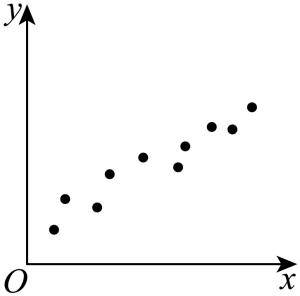
\includegraphics[width=.42\linewidth]{assets/asset-153-01.jpg}
\end{center}
\begin{choices}
  \item A
  \item B
  \item C
  \item D
\end{choices}
\begin{solution}
\textbf{答案：}A

\textbf{分析：}由点的分布特征可直接判断

\textbf{详解：}观察 4 幅图可知，A 图散点分布比较集中，且大体接近某一条直线，线性回归模型拟合效果比较好，呈现明显的正相关，$r$ 值相比于其他 3 图更接近 1. 故选 A.
\end{solution}
\end{question}

\begin{question}[points=5]
\textbf{来源：}2024 年 天津卷，第 13 题\par
$A,B,C,D,E$ 五种活动, 甲、乙都要选择三个活动参加. (1) 甲选到 $A$ 的概率为; 已知乙选了 $A$ 活动, 他再选择 $B$ 活动的概率为.
\fillin[{$\frac{3}{5}$, $\frac{1}{2}$}]
\begin{solution}
\textbf{答案：}$\frac{3}{5}$, $\frac{1}{2}$

\textbf{分析：}结合列举法或组合公式和概率公式可求甲选到 $A$ 的概率; 采用列举法或者条件概率公式可求乙选了 $A$ 活动, 他再选择 $B$ 活动的概率.

\textbf{详解：}解法一: 从五个活动中选三个的情况有 $C_5^3=10$ 种, 其中甲选到 $A$ 有 $C_4^2=6$ 种, 概率为 $\frac{6}{10}=\frac{3}{5}$. 乙选 $A$ 有 $C_4^2=6$ 种, 其中再选 $B$ 有 $C_3^1=3$ 种, 条件概率为 $\frac{3}{6}=\frac{1}{2}$. 解法二: $P(\text{甲选}A)=\frac{C_4^2}{C_5^3}=\frac{3}{5}$, $P(\text{乙选}B|\text{乙选}A)=\frac{C_3^1}{C_4^2}=\frac{1}{2}$.
\end{solution}
\end{question}

\begin{question}[points=5]
\textbf{来源：}2024 年 新高考II卷，第 4 题\par
某农业研究部门在面积相等的100块稻田上种植一种新型水稻，得到各块稻田的亩产量（单位：kg）并部分整理下表：



| 亩产量 | [900,950) | [950,1000) | [1000,1050) | [1100,1150) | [1150,1200) |

|--------|-----------|------------|-------------|-------------|-------------|

| 频数   | 6         | 12         | 18          | 24          | 10          |



据表中数据，结论中正确的是（ ）
\begin{choices}
  \item 100块稻田亩产量的中位数小于1050kg
  \item 100块稻田中亩产量低于1100kg的稻田所占比例超过80%
  \item 100块稻田亩产量的极差介于200kg至300kg之间
  \item 100块稻田亩产量的平均值介于900kg至1000kg之间
\end{choices}
\begin{solution}
\textbf{答案：}$C$

\textbf{分析：}计算出前三段频数即可判断A；计算出低于1100kg的频数，再计算比例即可判断B；根据极差计算方法即可判断C；根据平均值计算公式即可判断D.

\textbf{详解：}对于A，根据频数分布表可知，$6+12+18=36<50$，所以亩产量的中位数不小于1050kg，故A错误。对于B，亩产量不低于1100kg的频数为$24+10=34$，所以低于1100kg的稻田占比为$\dfrac{100-34}{100}=66\%$，故B错误。对于C，稻田亩产量的极差最大为$1200-900=300$，最小为$1150-950=200$，故C正确。对于D，由频数分布表可得，亩产量在[1050,1100)的频数为$100-(6+12+18+24+10)=30$，所以平均值为$\dfrac{1}{100}\times(6\times925+12\times975+18\times1025+30\times1075+24\times1125+10\times1175)=1067$，故D错误.
\end{solution}
\end{question}

\begin{question}[points=17]
\textbf{来源：}2024 年 新高考II卷，第 18 题\par
某投篮比赛分为两个阶段，每个参赛队由两名队员组成，比赛具体规则如下：第一阶段由参赛队中一名队员投篮3次，若3次都未投中，则该队被淘汰，比赛成绩为0分；若至少投中一次，则该队进入第二阶段，由该队的另一名队员投篮3次，每次投中得5分，未投中得0分。该队的比赛成绩为第二阶段的得分总和。某参赛队由甲、乙两名队员组成，设甲每次投中的概率为$p$，乙每次投中的概率为$q$，各次投中与否相互独立。

(1)若$p=0.4$，$q=0.5$，甲参加第一阶段比赛，求甲、乙所在队的比赛成绩不少于5分的概率。

(2)假设$0<p<q$，

(i)为使得甲、乙所在队的比赛成绩为15分的概率最大，应该由谁参加第一阶段比赛？

(ii)为使得甲、乙所在队的比赛成绩的数学期望最大，应该由谁参加第一阶段比赛？
\begin{solution}
\textbf{答案：}(1)$0.686$
(2)(i)由甲参加第一阶段比赛；(ii)由甲参加第一阶段比赛

\textbf{分析：}(1)根据对立事件的求法和独立事件的乘法公式即可得到答案；(2)(i)首先各自计算出$P_{\text{甲}}=[1-(1-p)^3]q^3$，$P_{\text{乙}}=[1-(1-q)^3]p^3$，再作差因式分解即可判断；(ii)首先得到$X$和$Y$的所有可能取值，再按步骤列出分布列，计算出各自期望，再次作差比较大小即可.

\textbf{详解：}（1）甲、乙所在队的比赛成绩不少于5分，则甲第一阶段至少投中1次，乙第二阶段也至少投中1次。比赛成绩不少于5分的概率$P=(1-0.6^3)(1-0.5^3)=0.686$。
（2）(i)若甲先参加第一阶段比赛，则甲、乙所在队的比赛成绩为15分的概率为$P_{\text{甲}}=[1-(1-p)^3]q^3$；若乙先参加第一阶段比赛，则甲、乙所在队的比赛成绩为15分的概率为$P_{\text{乙}}=[1-(1-q)^3]p^3$。因为$0<p<q$，所以$P_{\text{甲}}-P_{\text{乙}}=q^3-(q-pq)^3-p^3+(p-pq)^3=(q-p)(q^2+pq+p^2)+(p-q)[(p-pq)^2+(q-pq)^2+(p-pq)(q-pq)]=(p-q)(3p^2q^2-3p^2q-3pq^2)=3pq(p-q)(pq-p-q)=3pq(p-q)[(1-p)(1-q)-1]>0$，所以$P_{\text{甲}}>P_{\text{乙}}$，应该由甲参加第一阶段比赛。
(ii)若甲先参加第一阶段比赛，数学成绩$X$的所有可能取值为$0,5,10,15$，$P(X=0)=(1-p)^3+[1-(1-p)^3](1-q)^3$，$P(X=5)=[1-(1-p)^3]C_3^1q(1-q)^2$，$P(X=10)=[1-(1-p)^3]C_3^2q^2(1-q)$，$P(X=15)=[1-(1-p)^3]q^3$，所以$E(X)=15[1-(1-p)^3]q=15(p^3-3p^2+3p)q$。记乙先参加第一阶段比赛，数学成绩$Y$的所有可能取值为$0,5,10,15$，同理$E(Y)=15(q^3-3q^2+3q)p$。则$E(X)-E(Y)=15[pq(p+q)(p-q)-3pq(p-q)]=15(p-q)pq(p+q-3)$。因为$0<p<q$，则$p-q<0$，$p+q-3<1+1-3<0$，则$(p-q)pq(p+q-3)>0$，所以$E(X)>E(Y)$，应该由甲参加第一阶段比赛.
\end{solution}
\end{question}

\begin{question}[points=6]
\textbf{来源：}2024 年 新高考I卷，第 9 题\par
为了解推动出口后的亩收入（单位：万元）情况，从该种植区抽取样本，得到推动出口后亩收入的样本均值 $\overline{x}=2.1$，样本方差 $s^2=0.01$，已知该种植区以往的亩收入 $X$ 服从正态分布 $N(1.8,0.1^2)$，假设推动出口后的亩收入 $Y$ 服从正态分布 $N(\overline{x},s^2)$，则（ ）（若随机变量 $Z$ 服从正态分布 $N(\mu,\sigma^2)$，$P(Z<\mu+\sigma)\approx 0.8413$）
\begin{choices}
  \item $P(X>2)>0.2$
  \item $P(X>2)<0.5$
  \item $P(Y>2)>0.5$
  \item $P(Y>2)<0.8$
\end{choices}
\begin{solution}
\textbf{答案：}BC

\textbf{分析：}根据正态分布的 $3\sigma$ 原则以及正态分布的对称性即可解出.

\textbf{详解：}依题可知，$\overline{x}=2.1, s^2=0.01$，所以 $Y\sim N(2.1,0.1^2)$，故 $P(Y>2)=P(Y>2.1-0.1)=P(Y<2.1+0.1)\approx 0.8413>0.5$，C 正确，D 错误；因为 $X\sim N(1.8,0.1^2)$，所以 $P(X>2)=P(X>1.8+2\times0.1)$，因为 $P(X<1.8+0.1)\approx 0.8413$，所以 $P(X>1.8+0.1)\approx 1-0.8413=0.1587<0.2$，而 $P(X>2)=P(X>1.8+2\times0.1)<P(X>1.8+0.1)<0.2$，B 正确，A 错误.
\end{solution}
\end{question}

\begin{question}[points=5]
\textbf{来源：}2024 年 新高考I卷，第 14 题\par
甲、乙两人各有四张卡片，每张卡片上标有一个数字，甲的卡片上分别标有数字 $1,3,5,7$，乙的卡片上分别标有数字 $2,4,6,8$，两人进行四轮比赛，在每轮比赛中，两人各自从自己持有的卡片中随机选一张，并比较所选卡片上数字的大小，数字大的人得 $1$ 分，数字小的人得 $0$ 分，然后各自弃置此轮所选的卡片（弃置的卡片在此后的轮次中不能使用）.则四轮比赛后，甲的总得分不小于 $2$ 的概率为.
\fillin[{$\dfrac{1}{2}$}]
\begin{solution}
\textbf{答案：}$\dfrac{1}{2}$

\textbf{分析：}将每局的得分分别作为随机变量，然后分析其和随机变量即可.

\textbf{详解：}设甲在四轮游戏中的得分分别为 $X_1,X_2,X_3,X_4$，四轮的总得分为 $X$，对于任意一轮，甲乙两人在该轮出示每张牌的概率都均等，其中使得甲获胜的出牌组合有六种，从而甲在该轮获胜的概率 $P(X_k=1)=\dfrac{6}{4\times4}=\dfrac{3}{8}$，所以 $E(X_k)=\dfrac{3}{8}(k=1,2,3,4)$，从而 $E(X)=E(X_1+X_2+X_3+X_4)=4\times\dfrac{3}{8}=\dfrac{3}{2}$. 记 $p_k=P(X=k)(k=0,1,2,3)$. 如果甲得 $0$ 分，则组合方式是唯一的：必定是甲出 $1,3,5,7$ 分别对应乙出 $2,4,6,8$，所以 $p_0=\dfrac{1}{A_4^4}=\dfrac{1}{24}$；如果甲得 $3$ 分，则组合方式也是唯一的：必定是甲出 $1,3,5,7$ 分别对应乙出 $8,2,4,6$，所以 $p_3=\dfrac{1}{A_4^4}=\dfrac{1}{24}$. 而 $X$ 的所有可能取值是 $0,1,2,3$，故 $p_0+p_1+p_2+p_3=1$，$p_1+2p_2+3p_3=E(X)=\dfrac{3}{2}$. 所以 $p_1+p_2+\dfrac{1}{12}=1$，$p_1+2p_2+\dfrac{1}{8}=\dfrac{3}{2}$，两式相减得 $p_2+\dfrac{1}{24}=\dfrac{1}{2}$，故 $p_2+p_3=\dfrac{1}{2}$. 所以甲的总得分不小于 $2$ 的概率为 $p_2+p_3=\dfrac{1}{2}$.
\end{solution}
\end{question}

\section*{2025 年}

\begin{question}[points=5]
\textbf{来源：}2025 年 全国II卷，第 1 题\par
样本数据 $2$，$8$，$14$，$16$，$20$ 的平均数为（ ）
\begin{choices}
  \item $8$
  \item $9$
  \item $12$
  \item $18$
\end{choices}
\begin{solution}
\textbf{答案：}$C$

\textbf{分析：}由平均数的计算公式即可求解.

\textbf{详解：}样本数据 $2,8,14,16,20$ 的平均数为 $\frac{2+8+14+16+20}{5}=\frac{60}{5}=12$.
\end{solution}
\end{question}

\begin{question}[points=17]
\textbf{来源：}2025 年 全国II卷，第 19 题；次专题：数列\par
甲、乙两人进行乒乓球练习，每个球胜者得 $1$ 分，负者得 $0$ 分．设每个球甲胜的概率为 $p\left(\frac{1}{2}<p<1\right)$，乙胜的概率为 $q$，$p+q=1$，且各球的胜负相互独立，对正整数 $k\ge 2$，记 $p_k$ 为打完 $k$ 个球后甲比乙至少多得 $2$ 分的概率，$q_k$ 为打完 $k$ 个球后乙比甲至少多得 $2$ 分的概率．

（1）求 $p_3$，$p_4$（用 $p$ 表示）．

（2）若 $\frac{p_4-p_3}{q_4-q_3}=4$，求 $p$．

（3）证明：对任意正整数 $m$，$p_{2m+1}-q_{2m+1}<p_{2m}-q_{2m}<p_{2m+2}-q_{2m+2}$.
\begin{solution}
\textbf{答案：}（1）$p_3=p^3$，$p_4=p^3(4-3p)$
（2）$p=\frac{2}{3}$
（3）证明见解析

\textbf{分析：}（1）直接由二项分布概率计算公式即可求解；（2）由题意 $q_3=q^3$，$q_4=q^3(4-3q)$，联立 $\frac{p_4-p_3}{q_4-q_3}=4$，$p+q=1$ 即可求解；（3）首先 $p_{2m}-p_{2m+1}=C_{2m}^{m-1}p^{m+1}q^m$，$p_{2m+2}-p_{2m+1}=C_{2m+1}^{m}p^{m+2}q^m$，同理有 $q_{2m}-q_{2m+1}=C_{2m}^{m-1}q^{m+1}p^m$，$q_{2m+2}-q_{2m+1}=C_{2m+1}^{m}q^{m+2}p^m$，作差有 $p_{2m+1}-q_{2m+1}<p_{2m}-q_{2m}$，另一方面 $p_{2m+2}-p_{2m}=\frac{(2m+1)!}{m!(m+1)!}p^mq^m\cdot p\left(p-\frac{m}{2m+1}\right)$，且同理有 $q_{2m+2}-q_{2m}=\frac{(2m+1)!}{m!(m+1)!}p^mq^m\cdot q\left(q-\frac{m}{2m+1}\right)$，作差能得到 $p_{2m}-q_{2m}<p_{2m+2}-q_{2m+2}$，由此即可得证.

\textbf{详解：}（1）$p_3$ 为打完 $3$ 个球后甲比乙至少多得两分的概率，故只能甲胜三场，故 $p_3=C_3^3(1-p)^0p^3=p^3$；$p_4$ 为打完 $4$ 个球后甲比乙至少多得两分的概率，故甲胜三场或四场，故 $p_4=C_4^3(1-p)^1p^3+C_4^4(1-p)^0p^4=4p^3(1-p)+p^4=p^3(4-3p)$.
（2）由（1）得 $p_3=p^3$，$p_4=p^3(4-3p)$，同理 $q_3=q^3$，$q_4=q^3(4-3q)$，若 $\frac{p_4-p_3}{q_4-q_3}=4$，$p+q=1$，则 $\frac{p^3(4-3p)-p^3}{q^3(4-3q)-q^3}=\frac{3p^3(1-p)}{3q^3(1-q)}=\frac{p^3q}{q^3p}=\left(\frac{p}{q}\right)^2=4$，由于 $0<p,q<1$，所以 $p=2q=2(1-p)$，解得 $p=\frac{2}{3}$.
（3）我们有 $p_{2m}-p_{2m+1}=C_{2m}^{m-1}p^{m+1}q^m$，$p_{2m+2}-p_{2m+1}=C_{2m+1}^{m}p^{m+2}q^m$，同理有 $q_{2m}-q_{2m+1}=C_{2m}^{m-1}q^{m+1}p^m$，$q_{2m+2}-q_{2m+1}=C_{2m+1}^{m}q^{m+2}p^m$. 故 $p_{2m}-p_{2m+1}=C_{2m}^{m-1}p^{m+1}q^m\cdot 1$，$q_{2m}-q_{2m+1}=C_{2m}^{m-1}q^{m+1}p^m\cdot 1$，因为 $p>q$，所以 $p_{2m}-p_{2m+1}>q_{2m}-q_{2m+1}$，即 $p_{2m+1}-q_{2m+1}<p_{2m}-q_{2m}$. 另一方面，$p_{2m+2}-p_{2m}=\frac{(2m+1)!}{m!(m+1)!}p^mq^m\cdot p\left(p-\frac{m}{2m+1}\right)$，$q_{2m+2}-q_{2m}=\frac{(2m+1)!}{m!(m+1)!}p^mq^m\cdot q\left(q-\frac{m}{2m+1}\right)$，结合 $p\left(p-\frac{m}{2m+1}\right)-q\left(q-\frac{m}{2m+1}\right)=(p-q)(p+q)-\frac{m}{2m+1}(p-q)=(p-q)\left(1-\frac{m}{2m+1}\right)=\frac{(m+1)(p-q)}{2m+1}>0$，就能得到 $p_{2m+2}-p_{2m}>q_{2m+2}-q_{2m}$，即 $p_{2m}-q_{2m}<p_{2m+2}-q_{2m+2}$，证毕.
\end{solution}
\end{question}

\begin{question}[points=5]
\textbf{来源：}2025 年 全国I卷，第 14 题\par
一个箱子里有 $5$ 个相同的球，分别以 $1\sim5$ 标号，若有放回地取三次，记至少取出一次的球的个数 $X$，则数学期望 $E(X) =$ .
\fillin[{$\frac{61}{25}$}]
\begin{solution}
\textbf{答案：}$\frac{61}{25}$

\textbf{分析：}法一：根据题意得到 $X$ 的可能取值，再利用分步乘法原理与古典概型的概率公式求得 $X$ 的分布列，从而求得 $E(X)$；法二：利用数学期望的性质.

\textbf{详解：}法一：$X$ 的可能取值为 $1,2,3$，总共有 $5^3=125$ 种结果，$P(X=1)=\frac{5}{125}=\frac{1}{25}$，$P(X=2)=\frac{5\times4\times3}{125}=\frac{60}{125}=\frac{12}{25}$，$P(X=3)=\frac{5\times4\times3}{125}=\frac{60}{125}=\frac{12}{25}$，则 $E(X)=1\times\frac{1}{25}+2\times\frac{12}{25}+3\times\frac{12}{25}=\frac{61}{25}$. 法二：设 $X_i$ 表示球 $i$ 是否至少被取出一次，则 $X=\sum_{i=1}^5 X_i$，$E(X_i)=1-\left(\frac{4}{5}\right)^3 = \frac{61}{125}$，所以 $E(X)=5\times\frac{61}{125}=\frac{61}{25}$.
\end{solution}
\end{question}

\begin{question}[points=15]
\textbf{来源：}2025 年 全国I卷，第 15 题\par
为研究某疾病与超声波检查结果的关系，从做过超声波检查的人群中随机调查了 $1000$ 人，得到如下列联表：



| 超声波检查结果 | 正常 | 不正常 | 合计 |

|----------------|------|--------|------|

| 患该疾病 | 20 | 180 | 200 |

| 未患该疾病 | 780 | 20 | 800 |

| 合计 | 800 | 200 | 1000 |



（1）记超声波检查结果不正常者患该疾病的概率为 $P$，求 $P$ 的估计值；



（2）根据小概率值 $\alpha = 0.001$ 的独立性检验，分析超声波检查结果是否与患该疾病有关.



附 $\chi^2 = \frac{n(ad-bc)^2}{(a+b)(c+d)(a+c)(b+d)}$，



$P(\chi^2 \ge k)$ $0.005$ $0.010$ $0.001$



$k$ $3.841$ $6.635$ $10.828$
\begin{solution}
\textbf{答案：}（1）$\frac{9}{10}$；（2）有关

\textbf{分析：}（1）根据古典概型的概率公式即可求出；（2）根据独立性检验的基本思想，求出 $\chi^2$，然后与小概率值 $\alpha=0.001$ 对应的临界值 $10.828$ 比较，即可判断.

\textbf{详解：}（1）检查结果不正常的 $200$ 人中有 $180$ 人患病，所以 $P$ 的估计值为 $\frac{180}{200} = \frac{9}{10}$.
（2）零假设为 $H_0$：超声波检查结果与患病无关，根据表中数据可得 $\chi^2 = \frac{1000 \times (20\times20 - 780\times180)^2}{800\times200\times800\times200} = 765.625 > 10.828 = x_{0.001}$，根据小概率值 $\alpha=0.001$ 的 $\chi^2$ 独立性检验，推断 $H_0$ 不成立，即认为超声波检查结果与患该病有关，该推断犯错误的概率不超过 $0.001$.
\end{solution}
\end{question}

\begin{question}[points=4]
\textbf{来源：}2025 年 上海卷，第 6 题\par
\begin{center}

\begin{tabular}{ccccc}

已知随机变量 $X$ 的分布为 $\begin{pmatrix} 5 & 6 & 7 \\ 0.2 & 0.3 & 0.5 \end{pmatrix}$，则期望 $E[X] =$ ．

\end{tabular}

\end{center}
\fillin[{$6.3$}]
\begin{solution}
\textbf{答案：}$6.3$

\textbf{分析：}根据分布列结合期望公式可求期望.

\textbf{详解：}由题设有 $E[X] = 5 \times 0.2 + 6 \times 0.3 + 7 \times 0.5 = 1 + 1.8 + 3.5 = 6.3$ .
\end{solution}
\end{question}

\begin{question}[points=4]
\textbf{来源：}2025 年 上海卷，第 13 题\par
己知事件 $A$、$B$ 相互独立，事件 $A$ 发生的概率为 $P(A) = \frac{1}{2}$，事件 $B$ 发生的概率为 $P(B) = \frac{1}{2}$，则事件 $A \cap B$ 发生的概率 $P(A \cap B)$ 为（ ）
\begin{choices}
  \item $\frac{1}{8}$
  \item $\frac{1}{4}$
  \item $\frac{1}{2}$
  \item $0$
\end{choices}
\begin{solution}
\textbf{答案：}B

\textbf{分析：}根据独立事件的概率公式可求 $P(A \cap B)$ .

\textbf{详解：}因为 $A, B$ 相互独立，故 $P(A \cap B) = P(A)P(B) = \frac{1}{2} \times \frac{1}{2} = \frac{1}{4}$，故选：B.
\end{solution}
\end{question}

\begin{question}[points=14]
\textbf{来源：}2025 年 上海卷，第 17 题\par
2024 年东京奥运会，中国获得了男子 $4 \times 100$ 米混合泳接力金牌．以下是历届奥运会男子 $4 \times 100$ 米混合泳接力项目冠军成绩记录（单位：秒），数据按照升序排列．



206.78  207.46  207.95  209.34  209.35

210.68  213.73  214.84  216.93  216.93



(1) 求这组数据的极差与中位数；

(2) 从这 10 个数据中任选 3 个，求恰有 2 个数据在 211 以上的概率；

(3) 若比赛成绩 $y$ 关于年份 $x$ 的回归方程为 $\hat{y} = -0.311x + \hat{b}$，年份 $x$ 的平均数为 $2006$，预测 $2028$ 年冠军队的成绩（精确到 $0.01$ 秒）．
\begin{solution}
\textbf{答案：}(1) 极差 $10.15$，中位数 $210.015$； (2) $\frac{3}{10}$； (3) $204.56$ 秒

\textbf{分析：}(1) 由最长与最短用时可得极差，由中间两数平均数可得中位数； (2) 由古典概型概率公式可得； (3) 先求成绩平均数 $y$，再由 $(\bar{x}, \bar{y})$ 在回归直线上，代入方程可得 $\hat{b}$，再代入年份预测可得.

\textbf{详解：}(1) 由题意，数据的最大值为 $216.93$，最小值为 $206.78$，则极差为 $216.93 - 206.78 = 10.15$；数据中间两数为 $209.35$ 与 $210.68$，则中位数为 $\frac{209.35 + 210.68}{2} = 210.015$．故极差为 $10.15$，中位数为 $210.015$．
(2) 由题意，数据共 $10$ 个，$211$ 以上数据共有 $4$ 个，故设事件 $A = $“恰有 $2$ 个数据在 $211$ 以上”，则 $P(A) = \frac{\mathrm{C}_4^2 \cdot \mathrm{C}_6^1}{\mathrm{C}_{10}^3} = \frac{3}{10}$．故恰有 $2$ 个数据在 $211$ 以上的概率为 $\frac{3}{10}$．
(3) 由题意，成绩的平均数 $\bar{y} = \frac{206.78 + 207.46 + 207.95 + 209.34 + 209.35 + 210.68 + 213.73 + 214.84 + 216.93 + 216.93}{10} = 211.399$，由直线 $\hat{y} = -0.311x + \hat{b}$ 过 $(2006, 211.399)$，则 $\hat{b} = 211.399 + 0.311 \times 2006 = 835.265$，故回归直线方程为 $\hat{y} = -0.311x + 835.265$．当 $x = 2028$ 时，$\hat{y} = -0.311 \times 2028 + 835.265 = 204.557 \approx 204.56$．故预测 $2028$ 年冠军队的成绩为 $204.56$ 秒.
\end{solution}
\end{question}

\begin{question}[points=5]
\textbf{来源：}2025 年 天津卷，第 5 题\par
下列说法中错误的是（   ）
\begin{choices}
  \item 若$X \sim N(\mu, \sigma^2)$, 则$P(X \le \mu - \sigma) = P(X \ge \mu + \sigma)$
  \item 若$X \sim N(1, 2^2)$, $Y \sim N(2, 2^2)$, 则$P(X < 1) < P(Y < 2)$
  \item $r$越接近1，相关性越强
  \item $r$越接近0，相关性越弱
\end{choices}
\begin{solution}
\textbf{答案：}B

\textbf{分析：}根据正态分布以及相关系数的概念直接判断即可.

\textbf{详解：}对于A，根据正态分布对称性可知，$P(X \le \mu - \sigma) = P(X \ge \mu + \sigma)$, A说法正确；对于B，根据正态分布对称性可知，$P(X < 1) = P(Y < 2) = 0.5$, B说法错误；对于C和D，相关系数$r$越接近0，相关性越弱，越接近1，相关性越强，故C和D说法正确. 故选B.
\end{solution}
\end{question}

\begin{question}[points=5]
\textbf{来源：}2025 年 天津卷，第 13 题\par
小桐操场跑圈，一周2次，一次5圈或6圈. 第一次跑5圈或6圈的概率均为0.5，若第一次跑5圈，则第二次跑5圈的概率为0.4，6圈的概率为0.6；若第一次跑6圈，则第二次跑5圈的概率为0.6，4圈的概率为0.4. 小桐一周跑11圈的概率为；若一周至少跑11圈为动量达标，则连续跑4周，记合格周数为$X$, 则期望$E(X) = $.
\fillin[{$0.6；3.2$}]
\begin{solution}
\textbf{答案：}$0.6；3.2$

\textbf{分析：}先根据全概率公式计算求解空一，再求出概率根据二项分布数学期望公式计算求解.

\textbf{详解：}设小桐一周跑11圈为事件$A$, 设第一次跑5圈为事件$B$, 设第二次跑5圈为事件$C$, 则$P(A) = P(B)P(C|B) + P(\overline{B})P(\overline{C}|\overline{B}) = 0.5 \times 0.6 + 0.5 \times 0.6 = 0.6$；若至少跑11圈为运动量达标为事件$D$, $P(D) = P(A) + P(B)P(\overline{C}|B) = 0.6 + 0.5 \times 0.4 = 0.8$, 所以$X \sim B(4, 0.8)$, $E(X) = 4 \times 0.8 = 3.2$. 故答案为0.6；3.2.
\end{solution}
\end{question}

